\documentclass{article}

% Formatting
\DeclareUnicodeCharacter{2060}{\nolinebreak} % Prevent unicode (U+2060) error on local complile
\frenchspacing % No double spacing between sentences
\hbadness=1000000 % Turn off \hbox badness warnings
\linespread{1.2} % Set linespace


% Packages
\usepackage[a4paper, left=2.5cm, right=2.5cm, top=2.5cm, bottom=2.5cm]{geometry}
\usepackage{authblk} % For author formatting
\usepackage{caption} % For figure and table captions
\usepackage{cclicenses} % For creative commons license
\usepackage{float} % To force figure location after text
\usepackage{graphicx} % Adds more functionality to graphics for inclusion of figures
\usepackage{lscape} % For landscape pages
\usepackage{lineno} % Allows use of \linenumbers to add line numbers 
\usepackage{lmodern} % A scalable font - avoids erros due to non-sclabale fonts
\usepackage{longtable,booktabs}  % For tables
\usepackage{markdown} % allow use of markdown syntax
\usepackage{microtype} % 'Improved' typesetting
\usepackage[nottoc,numbib]{tocbibind} % Add references to table of contents
\usepackage{parskip} % Adds white space between paragraphs
\usepackage{pdflscape} % To create landscape pages that show as landscape in PDF viewer
\usepackage{ragged2e} % Better right ragged edges (allows hyphenation)
\usepackage{subcaption} % Allows use of subfigures
\usepackage[super]{natbib} % Citations using superscript
\usepackage{titlesec} % For title spacing
\usepackage[toc,page]{appendix}
\usepackage{url} % Tidy web links
\usepackage[utf8]{inputenc}
\usepackage{verbatim}
\usepackage{xcolor} % For coloured text
\usepackage{xurl} % For url but with more flexible linebreaking
\usepackage{placeins} % to use \FloatBarrier where want a hard break between content (to force and order of text and figures
% Info on wordcounts:
% https://www.overleaf.com/learn/how-to/Is_there_a_way_to_run_a_word_count_that_doesn%27t_include_LaTeX_commands%3F

% To include refs in word count:
%TC:incbib

\newcommand{\detailtexcount}[1]{%
  \immediate\write18{texcount -merge -sum -q #1.tex output.bbl > #1.wcdetail }%
  \verbatiminput{#1.wcdetail}%
}

% Count tables in wordcount (change to 0 0 if tables not included in word count)
%TC:group table 0 1
%TC:group tabular 1 

\begin{document}

% Ignore title and abstract in word count
%TC:ignore
\title{Thrombolysis: Are the results from the clinical trial meta-analysis seen in real life outcomes?  A machine learning study of the UK stroke registry.}


\renewcommand{\thefootnote}{\fnsymbol{footnote}}
\author[1,2]{Kerry Pearn}
\author[*1,2]{Michael Allen}
\author[1,2]{Anna Laws}
\author[1,2]{Martin James}

% Check affiliations - update RDE Name
\affil[1]{\footnotesize University of Exeter Medical School}
\affil[2]{\footnotesize NIHR South West Peninsula Applied Research Collaboration (ARC).}
\affil[*]{\footnotesize Corresponding author: m.allen@exeter.ac.uk}
\maketitle
%TC:endignore
%\include{sections/paper}

%TC:ignore
\section*{Abstract}

\textit{Introduction}: This study examines the effect of thrombolysis on discharge outcomes for ischaemic stroke patients in England and Wales using data from the UK prospective national stroke registry.

\textit{Patients and methods}: A total of 168,347 ischaemic stroke patients who attended one of 118 emergency stroke hospitals in England and Wales from 2016 to 2021 were extracted from the Sentinel Stroke National Audit Programme (SSNAP). We used explainable machine learning (XGBoost with SHAP) to examine the effect of patient characteristics, hospital attended, and use/time of thrombolysis on the odds of achieving a good outcome (being at or below any given modified Rankin Scale threshold). A linear regression model was fitted to the estimated effect of onset-to-treatment time on thrombolysis to permit comparison with clinical trial meta-analyses.

\textit{Results}: Thrombolysis was found to be associated with a statistically significant improvement in the odds of having a good outcome using any mRS threshold. Regression analysis predicted a maximum 2.5-fold improvement in odds of achieving mRS 0-1, with a decline to no treatment effect at 5 hours 28 minutes post-onset.

\textit{Discussion and Conclusion}: Our results confirm a beneficial effect of thrombolysis in a large prospective national stroke registry, and align closely with meta-analyses of clinical trials of thrombolysis both in terms of magnitude of effect and decline over time. This work also demonstrates the potential of applying explainable machine learning to observational data to extend understanding of stroke treatment outcomes for patient cohorts not included in the original clinical trials.

\section*{Plain English Summary}

\textbf{What is the problem?} Use of clot-busting treatment (`\textit{thrombolysis}') in stroke varies a great deal between hospitals.

\textbf{What did we know?} We knew that the largest cause of this variation was from how willing doctors are to use thrombolysis. Some doctors are worried that use of this treatment in the real world won’t have the same benefit that was predicted by the clinical trials.

\textbf{What did we not know?} We did not know what the effect of thrombolysis is in the real world across all types of patients where thrombolysis has been used. 

\textbf{What did we do?} We used explainable machine learning to learn how much patients benefit from thrombolysis in real world use. Machine learning finds patterns in large sets of data and can predict outcomes of patients. \textit{Explainable} machine learning allows us to sees what affects outcomes. We were particularly interested here in how use of thrombolysis affects outcomes.

\textbf{What did we find out?} We found out that thrombolysis was at least as effective in real world use as clinical trials predicted.


%TC:endignore

\section{Introduction}

% Include
% 1) What is the problem?
% 2) What do we know about low and varying use of thrombolysis
% 3) What do we not know
% 4) How are we addressing what we don't know

% 1) What is the problem?

Stroke remains one of the top three global causes of death and disability \cite{feigin_global_2021}. Despite reductions in age-standardised rates of stroke, ageing populations are driving an increase in the absolute number of strokes \cite{feigin_global_2021}. Across Europe, in 2017, stroke was estimated to cost healthcare systems \texteuro 27 billion, or 1.7\% of health expenditure \cite{luengo-fernandez_economic_2020}. The burden is increasing; it has been estimated that the number of stroke survivors aged 45 and over in the UK will more than double between 2015 and 2035 \cite{king_future_2020}.

Thrombolysis with recombinant tissue plasminogen activator, can significantly reduce disability after ischaemic stroke, provided it is given in the first few hours after stroke onset \cite{emberson_effect_2014}. 

Despite thrombolysis being of proven benefit in ischaemic stroke, use of thrombolysis varies significantly both between and within European countries \cite{aguiar_de_sousa_access_2019}. In England and Wales the Sentinel Stroke National Audit Programme (SSNAP) reported that in 2021/22, 20 years after the original European Medicines Agency licencing of alteplase for acute ischaemic stroke, thrombolysis rates varied from 1\% to 28\% of emergency stroke admissions between hospitals \cite{sentinel_national_stroke_audit_programme_ssnap_2022}, with a median rate of 10.4\% and an inter-quartile range of 8\%-13\%, against a 2019 NHS England long term plan that 20\% of patients with stroke should be receiving thrombolysis\cite{nhs_long_term_plan_2019}.

% 2) What do we know about low and varying use of thrombolysis

Studies have shown that reasons for low and varying thrombolysis rates are multi-factorial. Reasons include late presentation \cite{aguiar_de_sousa_access_2019}, lack of expertise \cite{aguiar_de_sousa_access_2019} or lack of clear protocols or training \cite{carter-jones_stroke_2011}, delayed access to specialists \cite{kamal_delays_2017}, and poor triage by ambulance or emergency department staff \cite{carter-jones_stroke_2011}. For many factors, the establishment of primary stroke centres has been suggested to improve the emergency care of patients with stroke and reduce barriers to thrombolysis \cite{carter-jones_stroke_2011}, with a centralised model of primary stroke centres leading to increased likelihood of thrombolysis \cite{lahr_proportion_2012, morris_impact_2014, hunter_impact_2013}. 

In addition to organisational factors, clinicians can have varying attitudes to which patients are suitable candidates for thrombolysis. In a discrete choice experiment \cite{de_brun_factors_2018}, 138 clinicians considered hypothetical patient vignettes, and responded as to whether they would give the patients thrombolysis. The authors concluded that there was considerable heterogeneity among respondents in their thrombolysis decision-making. Areas of difference were around whether to give thrombolysis to mild strokes, to older patients beyond 3 hours from stroke onset, and when there was pre-existing disability. We have also found, from interviews, that some clinicians express a lack of faith in the clinical trials of thrombolysis and demonstrated a reluctance to expressed a lack of faith in the clinical trials and reluctance to thrombolyse due to perceived risks of the procedure \cite{jarvie_stroke_2024}.

Based on national audit data from three years of emergency stroke admissions, we have previously built models of the emergency stroke pathway using clinical pathway simulation to examine the potential scale of the effect of changing two aspects of the stroke pathway performance (1. the in-hospital process speeds, and 2. the proportion of patients with a determined stroke onset time), and using machine learning to examine the effect of replicating clinical decision-making around thrombolysis from higher thrombolysing hospitals to lower thrombolysing hospitals \cite{allen_using_2022, allen_use_2022}. We showed that it would be credible to target an increase in average thrombolysis in England and Wales, from 11\% to 18\%, but that each hospital should have its own target, reflecting differences in local populations. We found that the largest increase in thrombolysis use would come from replicating thrombolysis decision-making practice from higher to lower thrombolysing hospitals.

In order to further understand the variation around thrombolysis decision-making, we employed explainable machine learning to understand how patient characteristics and the hospital attended affect the odds of a patient receiving thrombolysis\cite{pearn_what_2023}. We found that the odds of receiving thrombolysis varied 13 fold between hospitals, with lower thombolysing hospitals especially more likely to avoid thrombolysis in non-ideal candidates such as patients with mild stroke, or with pre-stroke disability.

% 3) What do we not know

Qualitative research has identified that clinicians from stroke teams with low thrombolysis use are concerned about the risk:benefit profile of thrombolysis \cite{jarvie_stroke_2024}. Confidence in the benefit of thrombolysis was especially lower in Emergency Department clinicians (as opposed to specialist stroke consultants), and there was more concern around patients that were seen as marginal candidates for thrombolysis, such as mild stroke.

There have been various observational studies which have provided further support for the effectiveness of thrombolysis \cite{wahlgren_thrombolysis_2007, wahlgren_thrombolysis_2008, manawadu_observational_2013, willeit_thrombolysis_2015}. None of these studies, however, were able to investigate the relationship between time-to-treatment and effectiveness compared to the clinical trial meta-analyses.

With the collection of clinical data for all emergency stroke admissions in England and Wales, and with the power of new explainable machine learning techniques, our aim was to build a predictive model of stroke outcomes, perform a large scale analysis of the benefit of thrombolysis in practice, and to compare the relationship between time-to-treatment and effectiveness with clinical trial results.
\section{Method}

\subsection{Data}

Data were retrieved for 168,347 emergency ischaemic stroke admissions to hospitals in England and Wales for six calendar years, 2016–2021 (inclusive), obtained from the Sentinel Stroke National Audit Programme (SSNAP). SSNAP prospectively collects clinical data from 100\% of acute hospitals in England and Wales, with case ascertainment estimated at $>$90\% when compared with administrative coding data. Data fields were provided for the hyperacute phase of the stroke pathway, up to and including the primary outcome of disability at inpatient discharge, recorded using the modified Rankin Scale (mRS) score. The data includes 118 acute stroke hospitals (each with at least 250 stroke admissions and which delivered thrombolysis to at least 10 patients in the study period), for patients that arrived at the hospital by ambulance after their stroke onset and did not go on to receive thrombectomy (rates of thrombectomy recorded in SSNAP increased from 0.7\% to 2.0\% of all stroke during this period).

\subsection{Feature selection}

The full dataset contained 57 features that described patient demographic and clinical characteristics, the acute stroke pathway, use/time of thrombolysis, and the stroke team they attended). We applied the feature selection results from Pearn \textit{et al}. \cite{pearn_are_2024}, which used modelling and discussions with clinicians to identify the influential features to include in the model.

Code and full results for feature selection may be found at \url{https://github.com/samuel-book/feature_selection_thrombolysis_outcome_ml_paper}

\subsection{Machine learning models}

We trained a set of six independent XGBoost models \cite{chen_xgboost_2016} to predict the likelihood of an ischaemic stroke patient attaining any given mRS threshold at discharge. For each mRS threshold, we refer to being at or lower than that threshold as a \textit{'same or better}' or '\textit{good outcome}'. We used 5-fold cross validation to test the accuracy of the model, and to test reproducibility of patterns detected (in 5-fold cross validation the data is split into 5 different 80:20 train/test splits with each patient being in one, and only one, test set). The results from the model fitted on the first k-fold split was used to investigate the relationships between feature values and their contribution to the predictions.

Code, and full results, for the machine learning work may be found at \url{https://github.com/samuel-book/thrombolysis_clinical_trials_ml_paper}

\subsection{Model accuracy}

For each of the six machine learning models, we report the model accuracy measured using the 5-fold model: percent correct and receiver operating characteristic area under curve (ROC-AUC).

\subsection{SHapley Additive exPlanation (SHAP) values}

SHAP values explain the contribution (as the change in log-odds) that each feature value has on the model’s prediction of achieving a good outcome at discharge \cite{lundberg_unified_2017}. SHAP values expressed as log-odds are additive (and so are preferred to probabilities, which are not additive, when examining the contribution of individual features to the final prediction). A SHAP model for each of the six machine learning models was created (one for each threshold of mRS). To illustrate how to interpret the SHAP value in our case, the target feature with a value of 1 represents a good outcome (being at or below any given mRS threshold), and a value 0 represents a worse outcome (being above any given mRS threshold). A positive SHAP value represents that the corresponding feature value increases the likelihood for that patient having a good outcome, and a negative SHAP value represents that the corresponding feature value reduces the likelihood for that patient having a good outcome. SHAP values can be assessed \textit{locally} at patient level, and \textit{globally} at patient cohort level to understand general patterns of how discharge outcomes differ by each of the patient, pathway, and hospital characteristics.

\subsection{Counterfactual treatment (what if patients had not received thrombolysis?)}

We used counterfactuals for each patient who received thrombolysis, to assess the contribution that thrombolysis made on the likelihood of a good outcome at discharge. Limiting this analysis to the 6,897 patients that receive thrombolysis in the first k-fold test set, we created their counterfactual case by setting the feature \textit{onset to treatment time} to 9,999 minutes (the same value used to train the model, for patients who did not receive thrombolysis) to represent the patient not receiving treatment, and used the model to predict their counterfactual outcome.

\subsubsection{The direct contribution of thrombolysis use to the shift in probability of a good outcome}

Taking the difference between the predicted log odds for a good outcome (mRS 0-1) at discharge, contributed by the \textit{onset to thrombolysis time} feature, when the patient received thrombolysis, and not, gave the predicted shift in likelihood of a good outcome at discharge with thrombolysis for each patient who received thrombolysis. We modelled the decay in effect of thrombolysis by fitting a linear regression model to the benefit of thrombolysis (log odds shift in attaining a good outcome) with time from onset to treatment (excluding patients treated after 300 minutes). The model used the definition of mRS 0-1 as a good outcome to match the definition used in the meta analysis of clinical trials \cite{emberson_effect_2014}. The analysis was applied to three patient cohorts: (1) all ischaemic strokes (n = 6,897), (2) severe ischaemic strokes, NIHSS 11+ (n = 2,897), (3) mild-moderate ischaemic strokes, NIHSS 0-10 (n = 4,000).

\section{Results}

\subsection{Descriptive statistics}

The 168,347 patients (who had onset-to-scan of within 255 minutes) attended 118 hospitals with admissions ranging from 358 to 4,559, with thrombolysis rates ranging from 5.9\% to 39.2\%. Of those 133,516 patients that did not receive thrombolysis, their range of disability at discharge was: 12\% mRS 0, 33\% mRS 0-1, 52\% mRS 0-2, 69\% mRS 0-3, 82\% mRS 0-4, and 88\% mRS 0-5 at discharge. Of those 34,831 patients that received thrombolysis, their range of disability at discharge was: 15\% mRS 0, 35\% mRS 0-1, 54\% mRS 0-2, 69\% mRS 0-3, 81\% mRS 0-4, and 86\% mRS 0-5.

Table \ref{tab:descriptive_stats} shows further descriptive statistics for the patients who received thrombolysis.

\begin{minipage}{1\textwidth}
\small
\renewcommand{\arraystretch}{1.2}
\begin{longtable}[]{@{}lllllllll@{}}
\caption{Descriptive statistics for patients who received thrombolysis}\label{tab:descriptive_stats}\\
\toprule
Patient feature &  Mean & Std Dev & Min & Q1 & Q2 & Q3 & Max\tabularnewline
\endhead
\midrule
Age (5 year age bands) & 73 & 13 & 37.5 & 62.5 & 72.5 & 82.5 & 92.5\tabularnewline
Proportion male & 0.55 & - & - & - & - & - & -\tabularnewline
Prior disability (mRS) & 0.8 & 1.2 & 0 & 0 & 0 & 1 & 5\tabularnewline
Stroke severity (NIHSS) & 10.8 & 7.0 & 0 & 5 & 9 & 16 & 42\tabularnewline
Onset to thrombolysis time (minutes) &  163 & 60 & 7 & 120 & 155 & 198 & 720\tabularnewline
Discharge disability (mRS) &  2.6 & 1.9 & 0 & 1 & 2 & 4 & 6\tabularnewline
\bottomrule

\end{longtable}
\normalsize
\end{minipage}

\subsection{Feature selection}

Using the results from Pearn \textit{el at}. \cite{pearn_are_2024}, we selected 7 features as inputs for the model to predict a patient's likelihood of a good outcome at discharge:

\begin{enumerate}
    \item Prior disability level: Disability level (mRS) before stroke
    \item Stroke severity: Stroke severity (NIHSS) on arrival
    \item Stroke team: Attended hospital
    \item Age: Age (as middle of 5 year age bands)
    \item Onset to thrombolysis time: Time from onset to receiving thrombolysis (minutes). This was set to 9,999 if the patient did not receive thrombolysis.
    \item Atrial fibrillation diagnosis: Patient had a diagnosis of atrial fibrillation (either on arrival or diagnosed during admission)
    \item Precise onset known: Onset time recorded was recorded as being precise time (as opposed to a best estimate)
\end{enumerate}


\subsection{Model accuracy}

With 7 input features, overall accuracy ranged from 77.6\% to 89.7\% across the six models (standard deviation across the 5 k-folds ranged from 0.001 to 0.002). This represented between 95-98\% of the accuracy that is obtained with all the features as inputs. ROC-AUC ranged from 0.852 to 0.893 across the six models (standard deviation across the 5 k-folds ranged from 0.001 to 0.002). Results were reproducible across the 5 k-folds, so further analysis was performed on the first k-fold split.


\subsection{Individual patient SHAP values}

SHAP values were calculated for each feature for each instance as how each value affects the log odds of having a good outcome at discharge. Figure \ref{fig:single_waterfall_with_ivt} shows a waterfall plot that illustrates the contribution from each feature value on the prediction for whether this individual patient had a good outcome (mRS 0-1) at discharge. This example patient (received thrombolysis at 165 minutes, known precisely, with no prior disability, 72.5 years old, had a moderate stroke, and attended hospital number 103) has a predicted 0.479 log odds (equivalent to 62\% probability) of having a good outcome (mRS 0-1) at discharge. For this patient, the two most influential features (that both increased the likelihood of having a good outcome, mRS 0-1) were prior disability (mRS 0) and onset to thrombolysis time (165 minutes).

\begin{figure}[!h]
    \centering%\captionsetup{width=.8\linewidth}%
      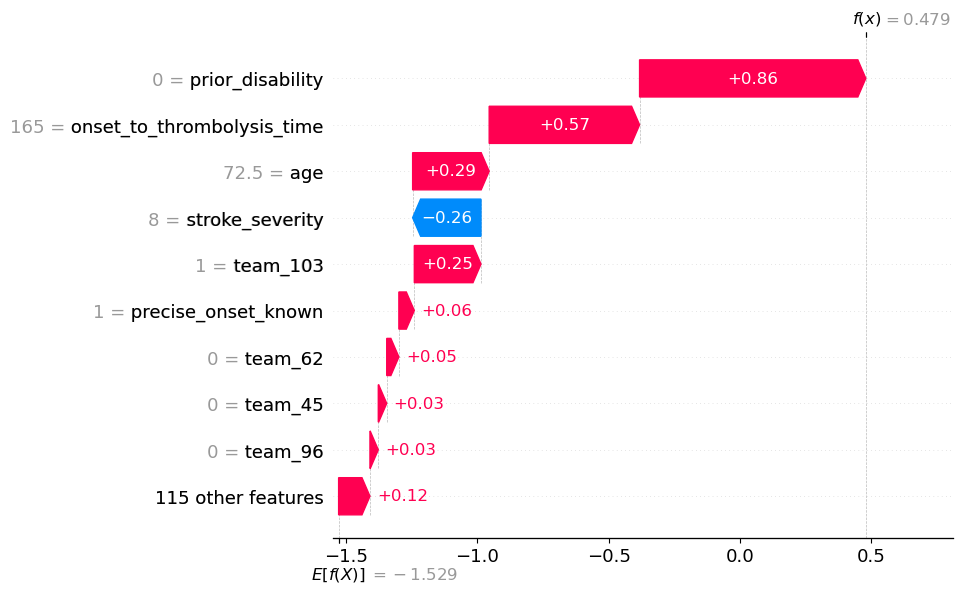
\includegraphics[width=0.95\linewidth]{./images/103_xgb_7_features_1fold_binary_waterfall_plot_patient16_with_IVT.png}\\
  \caption{The waterfall plot for a single patient showing the influence of the nine most influential feature values (y-axis) on the predicted likelihood of having a good outcome (mRS 0-1) on discharge (x-axis). Features are ranked in order of importance (top being most influential), with the contribution from the 10th ranked feature onwards being represented as a single contribution (\textit{115 other features}). The features with name prefix \textit{"team\_"} refers to a stroke team, where the value 1 represents the attended team, and the value 0 represents a team not attended (which may also have a small effect in the model). Each machine learning model applies the same SHAP base value (E[f(X)]) to each patient, this can be interpreted as the most likely outcome given no other knowledge of the instance. The sum of the SHAP base value and the SHAP values for each input feature equates to the overall predicted likelihood of having a good outcome on discharge, shown at the top of the plot (f(x)).}
    \label{fig:single_waterfall_with_ivt}
\end{figure}

\subsection{Global SHAP patterns}

For each patient in the test set we extracted SHAP values for each feature with its corresponding feature value. Figure \ref{fig:global_shap_mrs1} shows the relationship between feature values and the odds of a patient having a good outcome (mRS 0-1) at discharge (a positive SHAP value contributes to an increased likelihood, and a negative SHAP value contributes to a reduced likelihood). We see that low prior disability, lower stroke severity, younger age, receiving thrombolysis (and receiving it sooner after onset), and having no diagnosis of atrial fibrillation contributed to a patient more likely having a good outcome at discharge. Figure \ref{fig:global_shap_ott} focusses on the feature \textit{onset to thrombolysis time}, and its effect at reaching any disability threshold. As time from onset to treatment increased, the beneficial effect of thrombolysis decayed. For thresholds up to, and including, mRS 3, the median effect of thrombolysis remained positive, compared to not receiving thrombolysis, up until the maximum time of 720 minutes. For thresholds of mRS 4 and upwards, the median effect of thrombolysis became negative at longer onset-to-treatment times. This was especially apparent in how thrombolysis changed the overall odds of survival (mRS 0-5) where the median effect of thrombolysis became negative from about 155 minutes. Later thrombolysis may therefore increase the proportion of patients attaining mRS 0-3, but at the cost of some reduction in overall survival. Earlier thrombolysis improved the odds of survival. Figure \ref{fig:global_shap_hosp} shows the contribution from attending a specific hospital to predicting whether the patient had a good outcome at discharge, for each of the mRS threshold levels used to define a good outcome. As the threshold for having a good outcome becomes more inclusive, the range of the effect of the hospital attended had a reduced contribution on the prediction.


%%%%%%%% PUT ON SEPARATE A4 PAGE LANDSCAPE %%%%%%%%%%%

\begin{sidewaysfigure}[!ht]
    \centering
    \begin{subfigure}[b]{0.8\textwidth}
      \centering
      
\includegraphics[trim={0 0 0 1.2cm}, clip, width=1\textwidth]{./images/083_xgb_7_features_5fold_binary_shap_violin_mrs1_0kfold}\\
      \caption{The relationship between feature values and the prediction of whether a patient will have a good outcome (mRS 0-1) at discharge. SHAP base value for this model is -1.529.}
      \label{fig:global_shap_mrs1}
    \end{subfigure}
    \hfill
    \begin{subfigure}[b]{0.8\textwidth}
      \centering    
      
\includegraphics[width=1\textwidth]{./images/083_xgb_7_features_5fold_binary_shap_violin_onset_to_thrombolysis_time_0kfold.jpg}\\
%      
\includegraphics[trim={0 0 0 1.2cm}, clip, width=1\textwidth]{./images/083_xgb_7_features_5fold_binary_shap_violin_ss_0kfold}\\
      \caption{The relationship between onset to thrombolysis time and the prediction of whether a patient will have a good outcome at discharge, for each of the mRS scores used to define a good outcome.}
      \label{fig:global_shap_ott}
    \end{subfigure}
    \hfill
    \begin{subfigure}[b]{0.8\textwidth}
      \centering
      
\includegraphics[trim={0 0 0 1.2cm}, clip, width=1\textwidth]{./images/083_xgb_7_features_5fold_binary_hosp_shap_hist_mrs_0kfold}\\
      \caption{The contribution from attending a specific hospital to predicting whether the patient will have a good outcome at discharge, for each of the mRS scores used to define a good outcome}
      \label{fig:global_shap_hosp}
    \end{subfigure}
    \label{fig:global_shap}
  \caption{The relationship between feature values and SHAP values in predicting whether a patient will have a good outcome. Violin plots show the distribution of SHAP values across the patient population for each feature value, with the mid-line showing the median SHAP value.} 
\end{sidewaysfigure}


\subsection{Counterfactuals (what if patients had not received thrombolysis?)}

\subsubsection{For an individual patient}

Figure \ref{fig:double_waterfall} shows the waterfall plot for a single patient who received thrombolysis (figure \ref{fig:lhs_waterfall_with_ivt}), and its counterfactual case had the same patient not received thrombolysis (figure \ref{fig:rhs_waterfall_without_ivt}). This patient had a predicted 0.479 log odds (62\% probability) of having a good outcome (mRS 0-1) at discharge with thrombolysis, and -0.671 (34\% probability) without thrombolysis. By comparing the log odds contributed by the feature \textit{onset to thrombolysis time} in both cases (when the patient received thrombolysis, and not), we can isolate the predicted direct contribution to a good outcome of being given thrombolysis at a specified duration from stroke onset. For the patient in figure \ref{fig:double_waterfall} the predicted direct contribution to a good outcome (mRS 0-1) for being given thrombolysis at 165 minutes from stroke onset was 0.69 log odds (feature \textit{onset to thrombolysis time} contributed 0.57 log odds to the likelihood of a good outcome when given at 165 minutes, and -0.12 log odds when not given).

\begin{figure}[h]
    \centering
    \begin{subfigure}[t]{0.5\textwidth}
    \centering
    \captionsetup{width=.8\linewidth}%
      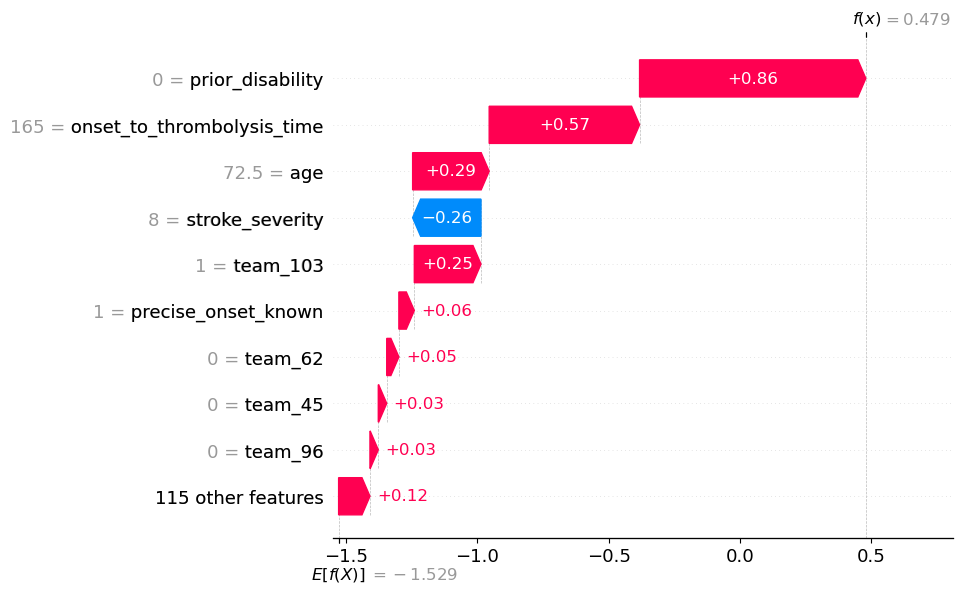
\includegraphics[width=1\linewidth]{./images/103_xgb_7_features_1fold_binary_waterfall_plot_patient16_with_IVT.png}\\
      \caption{Patient with original data (received thrombolysis at 165 minutes)                   
                                                                                }
      \label{fig:lhs_waterfall_with_ivt}
    \end{subfigure}%ults
    \begin{subfigure}[t]{0.5\textwidth}
    \centering
    \captionsetup{width=.8\linewidth}%
      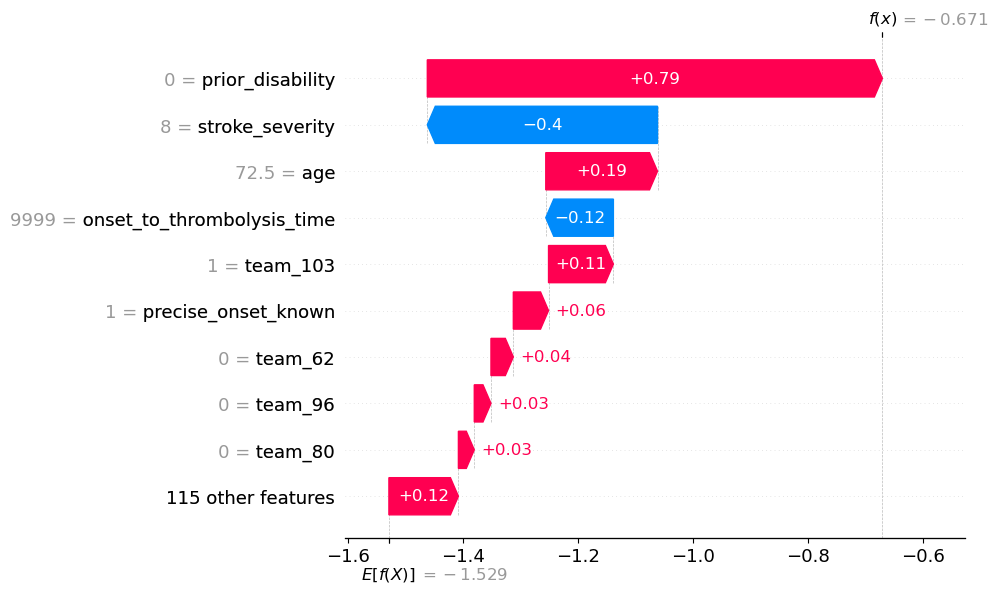
\includegraphics[width=1\linewidth]{./images/103_xgb_7_features_1fold_binary_waterfall_plot_patient16_without_IVT.png}\\
        \caption{Counterfactural case of the same patient not receiving thrombolysis (set onset-to-thrombolysis time to 9999 minutes)}
        \label{fig:rhs_waterfall_without_ivt}
    \end{subfigure}
  \caption{The waterfall plot for a single patient, and its counterfactual case, showing the influence of the nine most influential feature values (y-axis) on the predicted likelihood of having a good outcome (mRS 0-1) on discharge (x-axis). Features are ranked in order of importance (top being most influential), with the contribution from the 10th ranked feature onwards being represented as a single contribution (\textit{115 other features}). The features with name prefix \textit{"team\_"} refers to a stroke team, where the value 1 represents the attended team, and the value 0 represents a team not attended. Each machine learning model applies the same SHAP base value (E[f(X)]) to each patient, this can be interpreted as the most likely outcome given no other knowledge of the instance. The sum of the SHAP base value and the SHAP values for each input feature equates to the overall predicted likelihood of having a good outcome on discharge, shown at the top of the plot (f(x)).}
    \label{fig:double_waterfall}
\end{figure}

\subsubsection{For a cohort of patients}

Using the counterfactual results for all of the patients in the first k-fold test set that received thrombolysis (n = 6,897), figure \ref{fig:probability_shift} shows the shift in predicted probability of a good outcome at discharge, had they not received thrombolysis. For the majority of the cases, there is a greater probability for a good outcome with thrombolysis.

\begin{figure}[!h]
    \centering    \includegraphics[width=0.70\textwidth]%{./images/103_xgb_7_features_1fold_binary_probability_shift_counterfactuals_kfold0_no_max_time_mask}\\
{./images/103_xgb_7_features_1fold_binary_probability_shift_counterfactuals_kfold0_max_time_mask_400}\\

    \caption{The predicted probability of attaining a good outcome with and without thrombolysis, for those patients in the test population that received thrombolysis. Each plot shows the different mRS thresholds used to define a good outcome. The solid black line denotes no change (x=y). The white square shows the same patient across all six plots.}
    \label{fig:probability_shift}
\end{figure}

\subsubsection{The direct contribution of thrombolysis use to the shift in probability of a good outcome}

Using the counterfactual results for all of the patients in the first k-fold test set that received thrombolysis within 300 minutes from stroke onset (n = 6,796), figure \ref{fig:linear_regression_plots} shows a linear regression fitted to the shift in the contribution from receiving thrombolysis towards having a good outcome at discharge (mRS 0-1) with respect to the onset to thrombolysis time. We found, for all treated patients, that the effect of thrombolysis had declined to zero at 328 minutes, and the effect from thrombolysis was improving log odds of a good outcome by 0.90 if it were, theoretically, given at the time of stroke onset. We observed that the maximum theoretical effect of thrombolysis (if given at time of stroke onset) was greater for the severe stroke group (1.048 log odds) than the mild-moderate stroke group (0.771 log odds). However the effect of thrombolysis declined a little faster in the severe stroke group (reaching no effect at 314 minutes for severe stroke patients, compared to 351 minutes for mild-moderate stroke patients). Linear regression coefficients in all three patient groups were statistically significant (table \ref{fig:stats_table_mrs1}). 

\begin{figure}[!ht]
    \centering
    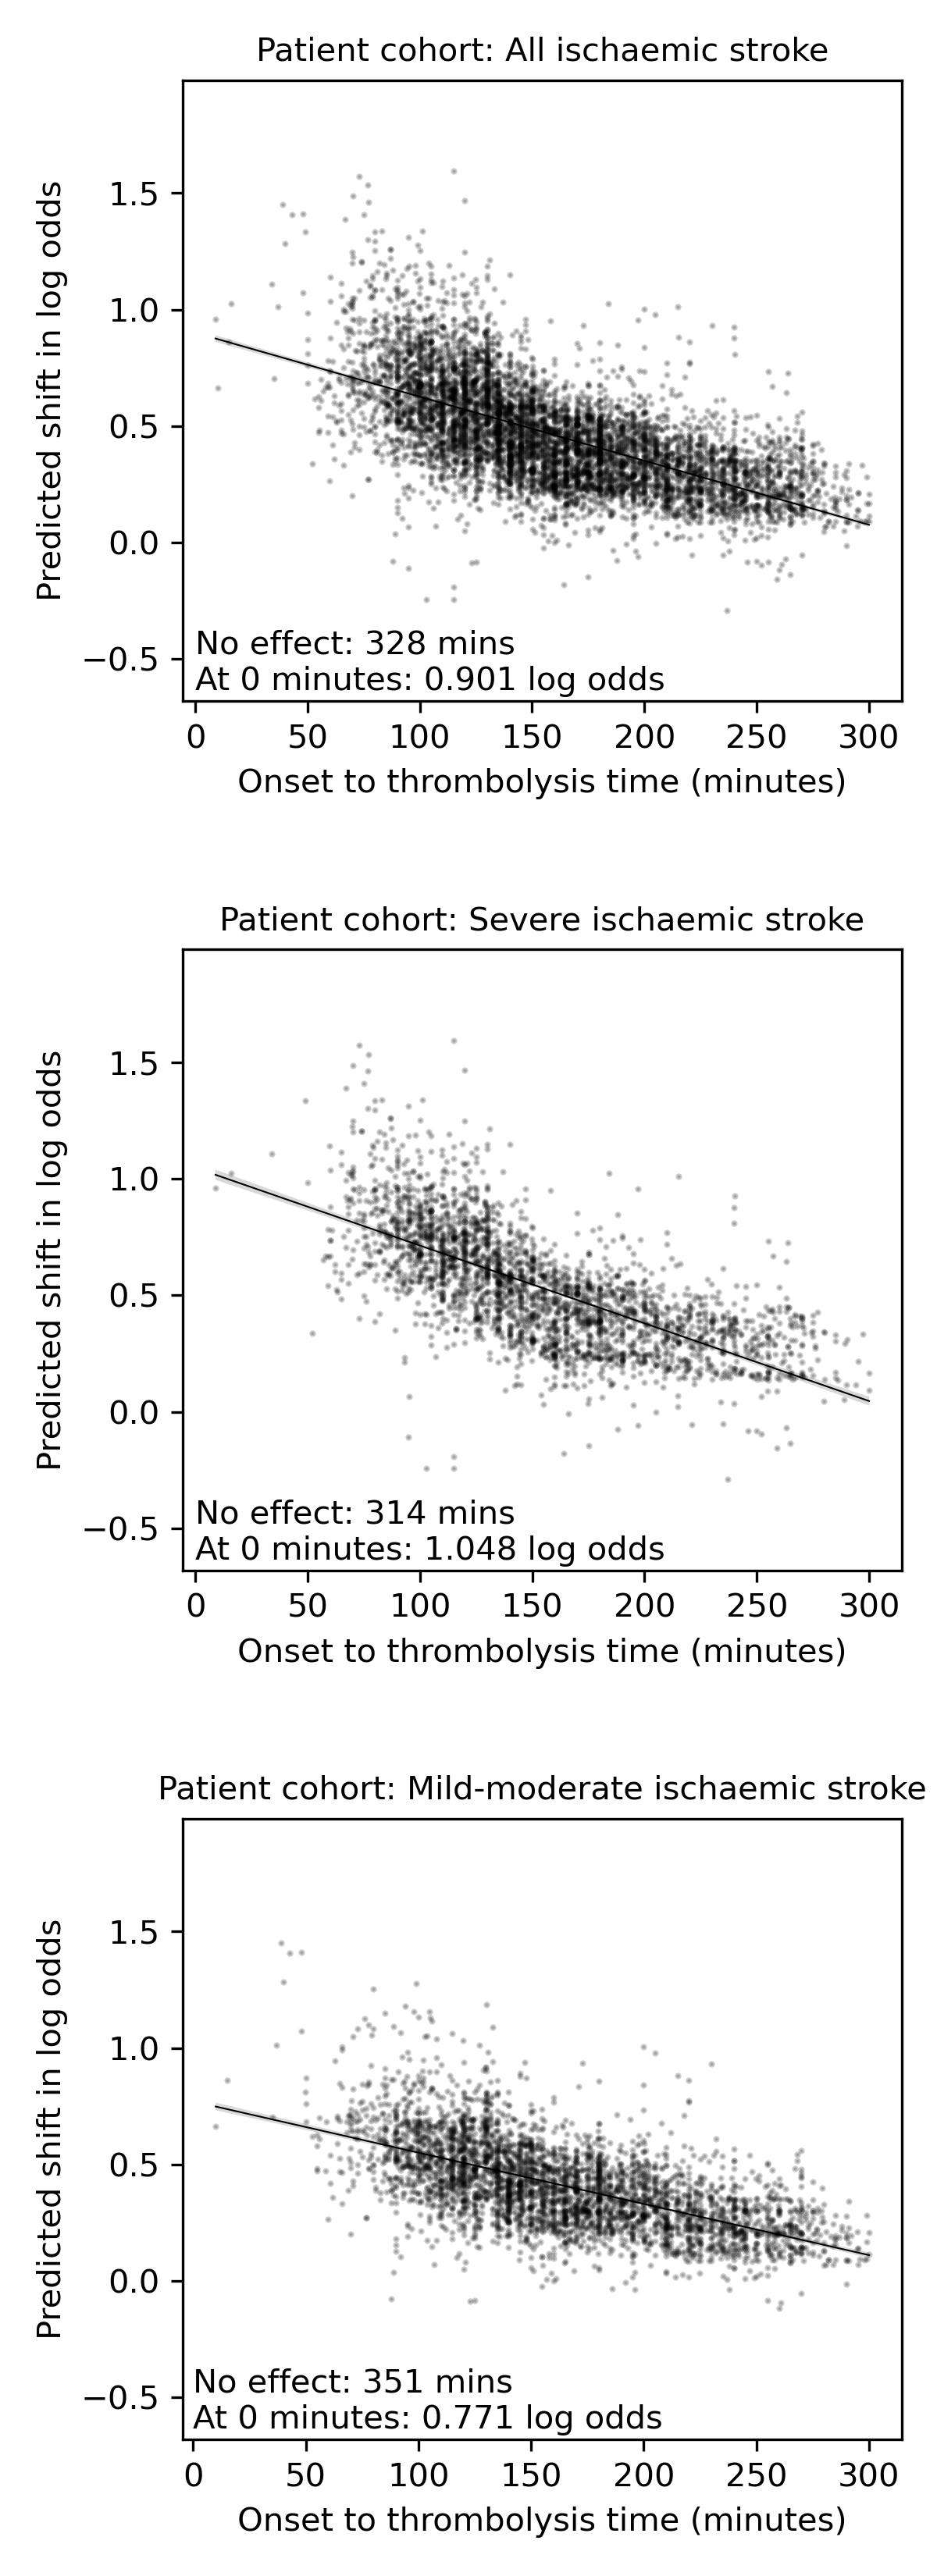
\includegraphics[width=0.50\textwidth]{./images/103_xgb_7_features_1fold_binary_improvement_logodds_mrs0_1_sns_subplots_ivt_shap_paper}\\
    \caption{A linear regression fit to the contribution from receiving thrombolysis on having a good outcome (mRS 0-1) at discharge, with respect to the onset to thrombolysis time (for patients treated within 300 minutes). Top: all treated stroke patients (n = 6,796); Middle: treated severe stroke patients, NIHSS 11+ (n = 2,856); Bottom: treated mild-moderate stroke patients, NIHSS 0-10 (n = 3,940).}
    \label{fig:linear_regression_plots}
\end{figure}


\begin{table}[!ht]
    \caption{Fitting linear regression to the shift in the contribution from receiving thrombolysis towards having a good outcome (mRS 0-1) at discharge with respect to the onset to thrombolysis (OTT) time. Linear regression statistics for different patient cohorts. We used NIHSS 0-10 to define mild-moderate strokes, and NIHSS 11+ to define severe strokes.}
    \centering
        \begin{tabular}{lllllllll}
        \toprule
         Ischaemic stroke type & Variables & coef & std err & t & P$>$$|$t$|$ & [0.025 & 0.975] \\ 
         \midrule
        All & Constant & 0.9012 & 0.007 & 132.519 & 0.000 & 0.888 & 0.915\\
        & OTT time (min) &  -0.0027  & 4.04e-05 & -68.058 & 0.000 & -0.003 & -0.003\\   
        \midrule
        Severe & Constant & 1.0476  &    0.011  & 96.746 & 0.000 & 1.026 & 1.069\\
        & OTT time (mins) & -0.0033 &  6.67e-05  & -50.042 & 0.000 & -0.003 & -0.003\\ 
        \midrule
        Mild-moderate & Constant &           0.7708 &     0.008   & 97.613 & 0.000 & 0.755 & 0.786\\
        & OTT (mins) &  -0.0022 &   4.57e-05 & -48.109 & 0.000 & -0.002 & -0.002\\
        \bottomrule
        \end{tabular}
      \label{fig:stats_table_mrs1}
\end{table}

\FloatBarrier

\section{Discussion}

%%%%%% INCLUDE %%%%%%

% Summarise main points

We built explainable machine learning models based on comprehensive prospective national stroke registry data capable of predicting disability outcome, at any given disability threshold, with high performance. The most influential factors that favoured being at or below any given disability threshold were lower pre-stroke disability, lower stroke severity, younger age, and use and speed of thrombolysis. The stroke team attended also had an effect on achieving any disability threshold, and that effect reduced with increasing disability at discharge. This could be due to 1) some hospitals discharging patients earlier with more disability e.g. with more community rehabilitation available, 2) effects of other hospital treatments on outcomes e.g. better/worse stroke unit care, or 3) hospitals assessing disability at discharge differently. From our model we cannot speculate further, but by including stroke team in the model we can adjust the model for these effects, allowing a clearer view of other patient features affecting outcome.

The model allows for counterfactual analysis, predicting outcomes with or without thrombolysis for any patient. In this analysis we focussed on predicting outcomes without thrombolysis, for those that actually received thrombolysis. In this way we investigate the effect of thrombolysis in those that did actually receive it. Using SHAP values, which explain the contribution of feature values to model prediction, we can also isolate the effect of thrombolysis. We found thrombolysis improved the odds of being at or below any given disability threshold, but the effect of thrombolysis was lower, and decayed to no-effect sooner, for outcomes of mRS $\leq$5 and $\leq$6. We found that the effect of thrombolysis was present for both mild-moderate and severe strokes, but with a larger effect in severe strokes. The findings from this study were remarkably similar to the meta-analysis of clinical trials \cite{emberson_effect_2014}, which extrapolate back to a 0.69 log odds (equivalent to an odds ratio of 2.0) improvement of being mRS 0-1 at stroke onset, with no effect after 378 minutes (6.3 hours). Our maximum theoretical improvement in log odds of achieving mRS 0-1 was a little higher at 0.90 (equivalent to an odds ratio of 2.5), with a decline to no-effect at 328 minutes (5.5 hours), indicating a somewhat steeper decline in effectiveness with time in our observational real-world study when compared to the original randomised data.  This is likely to be due to the licencing conditions for alteplase, in that the meta-analysis included randomised trials out to 6 hours from stroke onset \cite{emberson_effect_2014}, whereas the overwhelming majority of patients treated in the UK over the six-year study period were restricted to guideline-based eligibility within 4.5 hours \cite{intercollegiate_stroke_working_party_national_2016}.

% Compare to other work

The findings from this study were similar to the meta-analyses of clinical trials \cite{emberson_effect_2014}, which extrapolate back to a 0.69 log odds (equivalent to an odds ratio of 2.0) improvement of being mRS 0-1 at stroke onset, with no effect after 378 minutes (6.3 hours). Our maximum theoretical improvement in log odds improvement of being mRS 0-1 was a little higher, at 0.90 (equivalent to an odds ratio of 2.5), with a decline to no-effect at 328 minutes (5.5 hours).

Because of the size of the data available in the nationwide registry SSNAP, we are able to build more complex models than those derived from clinical trials, investigating stroke outcomes and benefit/disbenefit across a range of patient subgroups extending beyond the strict eligibility of randomised trials, and including comparisons of decision-making and outcomes between stroke teams.  This has, for example, allowed us to address the additional effect on outcomes from lower-thrombolysing teams adopting the less conservative practices in the use of thrombolysis found in higher thrombolysing teams. Companion papers to this paper explore these questions further \cite{pearn_are_2024, pearn_identifying_2024}. We have shown elsewhere that the majority of variation in thrombolysis rates between hospitals in the UK is accounted for by differences in clinical decision making, particularly around ‘less than ideal’ candidates for thrombolysis \cite{allen_use_2022, allen_using_2022, pearn_identifying_2024}.  The data in the current study show that in such patients there is a systematic disposition towards benefit at any level of disability outcome that supports the greater use of thrombolysis among patients not typically eligible for the original randomised trials.

% Clinical significance

The clinical significance of this work is that we have confirmed the net benefit of thrombolysis in a very large prospective national stroke registry that encompasses patients outside the strictly defined eligibility of the original randomised trials, and used sophisticated machine learning with SHAP to isolate the effect of thrombolysis from other patient characteristics that influence outcomes.  This provides significant reassurance that in real-world clinical practice, the anticipated benefits of thrombolysis are being delivered, even when treatment is deployed in a wider spectrum of patients than those represented in the randomised trials.

In summary, applying explainable machine learning to an observational data set demonstrated that the effectiveness of thrombolysis in the \textit{real world} appears to be at least as good as the clinical trials indicated. Our results should give stroke clinicians more confidence that the beneficial effect of thrombolysis is seen in real treatment populations. The size of the observational data set allows for more detailed analysis of the benefit of thrombolysis in subgroups of patients.

\subsection{Study limitations}

Though we are using a very large data set, our study necessarily has some limitations:

\begin{itemize}
    \item A group of more severely affected stroke patients who proceeded to receive thrombectomy has been excluded from the analysis, although during the six year study period endovascular intervention was increasing from a low base in the UK, and increased from 0.7\% to 2.0\% of all stroke.
    \item There is always a risk of inherent biases of an observational sample. Though our model has good accuracy, it remains possible that there are confounding patient characteristics that have an influence on the decision to treat, or the patient outcome, that are not measured in SSNAP.
    \item We have used the mRS at hospital discharge as our primary outcome, whereas the trials used the mRS at 90 days.  We know that the two are highly correlated \cite{elhabr_predicting_2021}, though individual patients may get better or worse between discharge and 90 days (possibly reflecting other aspects of care, such as community rehabilitation programmes).
\end{itemize}

\subsection{Further work}

Considering recent suggestions that thrombolysis should not be used in mild stroke \cite{braksick_thrombolysis_2024, zhang_intravenous_2024}, a more in-depth study of the observed effect of thrombolysis mild stroke, combining machine learning with causal inference methods such as propensity-score adjustment \cite{rosenbaum_central_1983} or target trial emulation \cite{hernan_target_2022}, would add to the evidence base around in this contentious group of patients.

%\include{sections/07_references}
%\include{sections/08_appendix}
%\newpage

%\section{References}
\bibliographystyle{naturemag}
%\bibliographystyle{plainnat}
%\bibliographystyle{unsrt}
%\bibliographystyle{unsrtnat}
\bibliography{references}

\section*{Acknowledgements}

We would like to thank the SAMueL project team (Lauren Asare, Julia Frost, Iain Lang, Kristin Liabo, Peter McMeekin, Keira Pratt-Boyden, Cathy Pope, Ken Stein, Penny Thompson, Rachel Jarvie) for their input into this work. We would also like to thank our Patient and Carer Involvement team led by Leon Farmer (David Burgess, Simon Douglas, Ian Hancock, Nicola Hancock, John Williams), and our expert advisory group (Ajay Bhalla, Gary Ford, Martin Utley).

\section*{Declaration of conflicting interests}

The authors declare no potential conflicts of interest with respect to the research, authorship, and/or publication of this article. 

\section*{Funding}

The authors disclose receipt of the following financial support for the research, authorship, and/or publication of this article: This research was funded by the National Institute for Health Research Applied Research Collaboration South West Peninsula and by the National Institute for Health Research Health and Social Care Delivery Research (HSDR) Programme [NIHR134326]. The views expressed in this publication are those of the authors and not necessarily those of the National Institute for Health Research or the Department of Health and Social Care. 

\section*{Informed consent and Ethics}

As we are using anonymised secondary data, collected for national audit, individual consent is not required. SSNAP has approval under section 251 of the NHS Health and Social Care Act (2006) to collect patient level data on the first six months of patient care (ECC 6- 02(FT3)/2012), without requiring individual patient consent. Access to SSNAP data is managed by the UK Healthcare Quality Improvement Partnership (HQIP), with this project being approved by HQIP (HQIP303). More information on SSNAPs use of patient data may be found at: \url{https://www.strokeaudit.org/ SupportFiles/Documents/Patient-area-documents/Fair-processingstatement-for-patients-v7-0.aspx}

As we are using anonymised secondary data, collected for national audit, used for service evaluation and improvement, no ethical approval is required (confirmed using the NHS Health Research Authority decision aid: https://www.hra-decisiontools.org.uk/ethics/).

\section*{Guarantor}

The corresponding author, Michael Allen, is the guarantor of the paper (PI on the NIHR project funding).




% Number for supplementary material
\newcommand{\beginsupplement}{
    \setcounter{section}{0}
    \renewcommand{\thesection}{S\arabic{section}}
    \setcounter{figure}{0}
    \renewcommand{\thefigure}{S\arabic{figure}}
    \setcounter{table}{0}
    \renewcommand{\thetable}{S\arabic{table}}
}
\beginsupplement

%TC:ignore
%\section{Supplementary material}

\subsection{Descriptive statistics}

\small
\renewcommand{\arraystretch}{1.3}
\begin{longtable}{p{7cm} p{1cm} p{0.8cm} p{0.8cm} p{0.8cm} p{0.8cm} p{0.8cm} p{0.8cm} p{0.8cm} p{0.8cm}}
\caption{Descriptive statistics for all patients arriving at each stroke team. The table shows summary statistics across all stroke teams.}\\
\toprule
\endhead
Statistic & Stroke teams & mean & Std Dev & min & 25\% & 50\% & 75\% & max\tabularnewline
\midrule
Yearly admissions & 119 & 509 & 208 & 95 & 372 & 489 & 627 & 1183\tabularnewline
Age (mean) & 119 & 74 & 2 & 65 & 73 & 75 & 76 & 78\tabularnewline
Proportion aged 80+ & 119 & 0.40 & 0.06 & 0.20 & 0.36 & 0.40 & 0.44 & 0.51\tabularnewline
Proportion male & 119 & 0.53 & 0.02 & 0.47 & 0.51 & 0.53 & 0.55 & 0.60\tabularnewline
Prior disability (mRS, mean) & 119 & 1.02 & 0.25 & 0.29 & 0.87 & 1.03 & 1.21 & 1.60\tabularnewline
Proportion prior disability (mRS) 0-2 & 119 & 0.81 & 0.05 & 0.67 & 0.78 & 0.81 & 0.84 & 0.97\tabularnewline
Proportion ischaemic stroke & 119 & 0.88 & 0.02 & 0.83 & 0.86 & 0.88 & 0.89 & 0.93\tabularnewline
Stroke severity (NIHSS, mean) & 119 & 7.0 & 1.0 & 4.6 & 6.3 & 7.2 & 7.8 & 9.1\tabularnewline
Proportion with known onset & 119 & 0.68 & 0.14 & 0.43 & 0.58 & 0.67 & 0.76 & 1.00\tabularnewline
Onset-to-arrival time (minutes, median) & 119 & 204 & 76 & 109 & 155 & 180 & 224 & 466\tabularnewline
Proportion arriving within 4 hours known onset & 119 & 0.38 & 0.06 & 0.19 & 0.34 & 0.38 & 0.43 & 0.51\tabularnewline
Proportion with precisely known onset & 119 & 0.33 & 0.11 & 0.01 & 0.28 & 0.34 & 0.39 & 0.63\tabularnewline
Proportion onset during sleep & 119 & 0.14 & 0.06 & 0.00 & 0.09 & 0.14 & 0.17 & 0.34\tabularnewline
Proportion arrive by ambulance & 119 & 0.78 & 0.07 & 0.47 & 0.76 & 0.79 & 0.82 & 0.92\tabularnewline
Call-to-ambulance arrival time (minutes, median) & 113 & 22 & 10 & 13 & 17 & 20 & 24 & 103\tabularnewline
Ambulance on scene time (median) & 113 & 31 & 3 & 20 & 28 & 31 & 33 & 41\tabularnewline
Ambulance conveyance time (minutes, median) & 113 & 18 & 5 & 10 & 15 & 17 & 21 & 37\tabularnewline
Arrival-to-scan time (minutes, median) & 119 & 53 & 21 & 13 & 39 & 51 & 63 & 129\tabularnewline
Proportion receiving thrombolysis & 119 & 0.115 & 0.034 & 0.021 & 0.092 & 0.110 & 0.136 & 0.245\tabularnewline
Scan-to-thrombolysis time (minutes, median) & 119 & 34 & 10 & 14 & 28 & 34 & 41 & 72\tabularnewline
Discharge disability (mRS, mean) & 119 & 2.641 & 0.352 & 1.361 & 2.413 & 2.699 & 2.900 & 3.320\tabularnewline
Proportion discharged mRS 0-2 & 119 & 0.524 & 0.095 & 0.293 & 0.454 & 0.522 & 0.594 & 0.799\tabularnewline
Proportion discharged mRS 5-6 & 119 & 0.195 & 0.037 & 0.095 & 0.170 & 0.198 & 0.218 & 0.287\tabularnewline
\bottomrule
\label{tab:hospital_stats_1}
\end{longtable}
\normalsize

\small
\begin{longtable}{p{7cm} p{1cm} p{0.8cm} p{0.8cm} p{0.8cm} p{0.8cm} p{0.8cm} p{0.8cm} p{0.8cm} p{0.8cm}}
\caption{Descriptive statistics for patients arriving at each stroke team, for patients arriving within 4 hours of known stroke onset. The table shows summary statistics across all stroke teams.}\\
\toprule
\endhead
Statistic & Stroke teams & mean & Std Dev & min & 25\% & 50\% & 75\% & max\tabularnewline
\midrule
Yearly admissions & 119 & 193 & 78 & 28 & 139 & 183 & 241 & 428\tabularnewline
Age (mean) & 119 & 75 & 2 & 66 & 73 & 75 & 76 & 79\tabularnewline
Proportion aged 80+ & 119 & 0.41 & 0.06 & 0.23 & 0.37 & 0.41 & 0.45 & 0.57\tabularnewline
Proportion male & 119 & 0.53 & 0.03 & 0.45 & 0.51 & 0.53 & 0.55 & 0.64\tabularnewline
Prior disability (mRS, mean) & 119 & 1.04 & 0.25 & 0.37 & 0.88 & 1.04 & 1.22 & 1.60\tabularnewline
Proportion prior disability (mRS) 0-2 & 119 & 0.80 & 0.06 & 0.66 & 0.77 & 0.81 & 0.83 & 0.95\tabularnewline
Proportion ischaemic stroke & 119 & 0.85 & 0.03 & 0.75 & 0.84 & 0.85 & 0.87 & 0.94\tabularnewline
Stroke severity (NIHSS, mean) & 119 & 8.9 & 1.1 & 6.4 & 8.2 & 9.0 & 9.7 & 11.4\tabularnewline
Proportion with known onset & 119 & 1.00 & 0.00 & 1.00 & 1.00 & 1.00 & 1.00 & 1.00\tabularnewline
Onset-to-arrival time (minutes, median) & 119 & 105 & 9 & 85 & 100 & 105 & 111 & 132\tabularnewline
Proportion arriving within 4 hours known onset & 119 & 1.00 & 0.00 & 1.00 & 1.00 & 1.00 & 1.00 & 1.00\tabularnewline
Proportion with precisely known onset & 119 & 0.62 & 0.17 & 0.02 & 0.54 & 0.66 & 0.75 & 0.91\tabularnewline
Proportion onset during sleep & 119 & 0.05 & 0.05 & 0.00 & 0.01 & 0.03 & 0.06 & 0.30\tabularnewline
Proportion arrive by ambulance & 119 & 0.89 & 0.07 & 0.54 & 0.87 & 0.91 & 0.93 & 0.98\tabularnewline
Call-to-ambulance arrival time (minutes, median) & 110 & 19 & 5 & 8 & 16 & 18 & 21 & 51\tabularnewline
Ambulance on scene time (median) & 110 & 28 & 4 & 20 & 26 & 28 & 31 & 46\tabularnewline
Ambulance conveyance time (minutes, median) & 110 & 17 & 4 & 9 & 14 & 16 & 20 & 28\tabularnewline
Arrival-to-scan time (minutes, median) & 119 & 27 & 11 & 4 & 21 & 28 & 34 & 100\tabularnewline
Proportion receiving thrombolysis & 119 & 0.293 & 0.070 & 0.111 & 0.250 & 0.282 & 0.333 & 0.534\tabularnewline
Scan-to-thrombolysis time (minutes, median) & 119 & 34 & 10 & 14 & 28 & 34 & 40 & 71\tabularnewline
Discharge disability (mRS, mean) & 119 & 2.803 & 0.353 & 1.507 & 2.609 & 2.837 & 3.039 & 3.663\tabularnewline
Proportion discharged mRS 0-2 & 119 & 0.494 & 0.094 & 0.209 & 0.424 & 0.495 & 0.554 & 0.771\tabularnewline
Proportion discharged mRS 5-6 & 119 & 0.236 & 0.045 & 0.138 & 0.208 & 0.231 & 0.256 & 0.420\tabularnewline
\bottomrule
\label{tab:hospital_stats_2}
\end{longtable}
\normalsize

\small
\begin{longtable}{p{7cm} p{1cm} p{0.8cm} p{0.8cm} p{0.8cm} p{0.8cm} p{0.8cm} p{0.8cm} p{0.8cm} p{0.8cm}}
\caption{Descriptive statistics for patients arriving at each stroke team, for patients arriving by ambulance within 4 hours of known stroke onset. The table shows summary statistics across all stroke teams.}\\
\toprule
\endhead
Statistic & Stroke teams & mean & Std Dev & min & 25\% & 50\% & 75\% & max\tabularnewline
\midrule
Yearly admissions & 119 & 173 & 74 & 15 & 125 & 163 & 227 & 400\tabularnewline
Age (mean) & 119 & 75 & 2 & 66 & 74 & 76 & 77 & 81\tabularnewline
Proportion aged 80+ & 119 & 0.43 & 0.06 & 0.24 & 0.39 & 0.43 & 0.47 & 0.62\tabularnewline
Proportion male & 119 & 0.52 & 0.03 & 0.45 & 0.51 & 0.52 & 0.54 & 0.60\tabularnewline
Prior disability (mRS, mean) & 119 & 1.10 & 0.25 & 0.46 & 0.94 & 1.09 & 1.26 & 1.66\tabularnewline
Proportion prior disability (mRS) 0-2 & 119 & 0.79 & 0.06 & 0.65 & 0.75 & 0.79 & 0.83 & 0.93\tabularnewline
Proportion ischaemic stroke & 119 & 0.85 & 0.03 & 0.75 & 0.83 & 0.85 & 0.87 & 0.94\tabularnewline
Stroke severity (NIHSS, mean) & 119 & 9.4 & 1.2 & 6.7 & 8.6 & 9.5 & 10.2 & 12.2\tabularnewline
Proportion with known onset & 119 & 1.00 & 0.00 & 1.00 & 1.00 & 1.00 & 1.00 & 1.00\tabularnewline
Onset-to-arrival time (minutes, median) & 119 & 106 & 10 & 84 & 99 & 105 & 112 & 151\tabularnewline
Proportion arriving within 4 hours known onset & 119 & 1.00 & 0.00 & 1.00 & 1.00 & 1.00 & 1.00 & 1.00\tabularnewline
Proportion with precisely known onset & 119 & 0.62 & 0.17 & 0.02 & 0.54 & 0.65 & 0.75 & 0.92\tabularnewline
Proportion onset during sleep & 119 & 0.05 & 0.05 & 0.00 & 0.01 & 0.03 & 0.06 & 0.33\tabularnewline
Proportion arrive by ambulance & 119 & 1.00 & 0.00 & 1.00 & 1.00 & 1.00 & 1.00 & 1.00\tabularnewline
Call-to-ambulance arrival time (minutes, median) & 110 & 19 & 5 & 8 & 16 & 18 & 21 & 51\tabularnewline
Ambulance on scene time (median) & 110 & 28 & 4 & 20 & 26 & 28 & 31 & 46\tabularnewline
Ambulance conveyance time (minutes, median) & 110 & 17 & 4 & 9 & 14 & 16 & 20 & 28\tabularnewline
Arrival-to-scan time (minutes, median) & 119 & 26 & 11 & 4 & 20 & 25 & 33 & 95\tabularnewline
Proportion receiving thrombolysis & 119 & 0.300 & 0.072 & 0.130 & 0.252 & 0.289 & 0.345 & 0.537\tabularnewline
Scan-to-thrombolysis time (minutes, median) & 119 & 34 & 10 & 13 & 27 & 33 & 40 & 73\tabularnewline
Discharge disability (mRS, mean) & 119 & 2.926 & 0.352 & 1.867 & 2.717 & 2.928 & 3.150 & 3.819\tabularnewline
Proportion discharged mRS 0-2 & 119 & 0.465 & 0.096 & 0.184 & 0.398 & 0.462 & 0.524 & 0.696\tabularnewline
Proportion discharged mRS 5-6 & 119 & 0.254 & 0.051 & 0.147 & 0.221 & 0.253 & 0.280 & 0.486\tabularnewline
\bottomrule
\label{tab:hospital_stats_3}
\end{longtable}
\normalsize


\subsection{Feature selection}

\textbf{Summary of findings}

Model with all features
The model performance with all 58 features is:
* AUC: 0.818 (std across 5 kfolds: 0.001)
* Accuracy: 0.440 (std across 5 kfolds: 0.002)
* Accuracy within one: 0.760 (std across 5 kfolds: 0.002)

\textbf{Sequentially selecting features}
Sequentially chose features up to 25 features. We saw that once 14 features we selected, the model choose a feature (infarction) that is the same value for all patients, hence no more information was being obtained beyond this point:
Feature  1: prior\_disability, AUC: 0.687
Feature  2: stroke\_severity, AUC: 0.770
Feature  3: stroke\_team, AUC: 0.800
Feature  4: age, AUC: 0.806
Feature  5: year, AUC: 0.811
Feature  6: nihss\_arrival\_loc, AUC: 0.814
Feature  7: scan\_to\_thrombolysis\_time, AUC: 0.816
Feature  8: thrombolysis\_no\_but\_improving, AUC: 0.817
Feature  9: nihss\_arrival\_best\_language, AUC: 0.818
Feature 10: new\_afib\_diagnosis, AUC: 0.818
Feature 11: nihss\_arrival\_sensory, AUC: 0.819
Feature 12: atrial\_fibrillation, AUC: 0.819
Feature 13: nihss\_arrival\_facial\_palsy, AUC: 0.819
Feature 14: thrombolysis\_no\_but\_other\_medical, AUC: 0.819
Feature 15: infarction, AUC: 0.819
Feature 16: arrive\_by\_ambulance, AUC: 0.819
Feature 17: nihss\_arrival\_motor\_arm\_left, AUC: 0.819
Feature 18: thrombolysis\_no\_but\_comorbidity, AUC: 0.819
Feature 19: nihss\_arrival\_loc\_questions, AUC: 0.819
Feature 20: nihss\_arrival\_motor\_arm\_right, AUC: 0.819
Feature 21: nihss\_arrival\_best\_gaze, AUC: 0.820
Feature 22: thrombolysis\_no\_but\_too\_mild\_severe, AUC: 0.820
Feature 23: diabetes, AUC: 0.820
Feature 24: thrombolysis\_no\_but\_haemorrhagic, AUC: 0.820
Feature 25: thrombolysis\_no\_but\_medication, AUC: 0.820

\textbf{Features chosen for the predictive model}
We will include these 7 features in our model (reasoning given below):
Feature  1: prior\_disability
Feature  2: stroke\_severity
Feature  3: stroke\_team
Feature  4: age
Feature  5: onset\_to\_thrombolysis\_time
Feature  6: any\_afib\_diagnosis
Feature  7: precise\_onset\_known

\textbf{Additional experiments to inform choice of features}

To inform us further about which features to include in our model, we carried out some additional experiments (in other notebooks). Here is what we learnt, and our feature selection choice based on this.

\textbf{Why we chose these 7 features:}
* prior\_disability (easy selection choice)
* stroke\_severity (checked the impact of using the separate NIHSS features instead - decided including stroke severity captured the information)
* stroke\_team (easy selection choice)
* age (easy selection choice)
* onset\_to\_thrombolysis\_time (scan\_to\_thrombolysis\_time is a selected feature, however the feature onset-to-thrombolysis time is a more useful feature to include as it aligns with other research and the clinical focus.We compared the SHAP plots from models that included either (and neither) of these duration features. Across the three models, the other features (age, prior disability, stroke severity) are not affected by the inclusion of either duration feature, nor is any performance accuracy lost)
* any\_afib\_diagnosis (Both new\_afib\_diagnosis and atrial\_fibrillation featrures are in the list above, and we have seen that an atrial fibrillation diagnosis contributes for the mRS6 outcome. We will include any\_afib\_diagnosis as this includes both of the other atrial fibrillation features information. We compared the SHAP plots from models that included one of these atrial fibrillation diagnosis features (and none). Across those models, the other features (age, prior disability, stroke severity) are not affected by the inclusion of which atrial fibrillation feature, nor is any performance accuracy lost).
* precise\_onset\_known (Not included in the feature selection list, however may be useful to include so people can see whether it makes a significant difference to outcomes, as this is often a discussion point amongst clinicians)

\textbf{Why we didn't include these features:}
* YEAR: Any data from beyond 2021 (the latest year in the dataset), the model has yet to see any information about that year. If the decision tree treats the ”Year” feature as a numerical value, any future year will be grouped along with year 2021 for each split - check how the model is treating the Year feature.

We reran feature selection excluding the feature "stroke team" as an option. The feature "Year" was now not a selected features. Here are those results:

There are 56 features
All features, AUC: 0.786 (std across 5 kfolds: 0.001)
All features, accuracy: 0.387 (std across 5 kfolds: 0.003)
All features, accuracy within one: 0.734 (std across 5 kfolds: 0.003)

Feature  1: prior\_disability, AUC: 0.687
Feature  2: stroke\_severity, AUC: 0.770
Feature  3: age, AUC: 0.777
Feature  4: nihss\_arrival\_loc, AUC: 0.779
Feature  5: scan\_to\_thrombolysis\_time, AUC: 0.780
Feature  6: thrombolysis\_no\_but\_improving, AUC: 0.782
Feature  7: nihss\_arrival\_best\_language, AUC: 0.783
Feature  8: thrombolysis\_no\_but\_other\_medical, AUC: 0.783
Feature  9: nihss\_arrival\_sensory, AUC: 0.784
Feature 10: nihss\_arrival\_facial\_palsy, AUC: 0.784
Feature 11: nihss\_arrival\_limb\_ataxia, AUC: 0.784
Feature 12: nihss\_arrival\_motor\_arm\_left, AUC: 0.785
Feature 13: nihss\_arrival\_best\_gaze, AUC: 0.785
Feature 14: diabetes, AUC: 0.785
Feature 15: thrombolysis\_no\_but\_comorbidity, AUC: 0.785
Feature 16: nihss\_arrival\_motor\_arm\_right, AUC: 0.786
Feature 17: thrombolysis\_no\_but\_too\_mild\_severe, AUC: 0.786
Feature 18: onset\_during\_sleep, AUC: 0.786
Feature 19: precise\_onset\_known, AUC: 0.786
Feature 20: atrial\_fibrillation, AUC: 0.786
Feature 21: infarction, AUC: 0.786
Feature 22: arrive\_by\_ambulance, AUC: 0.786
Feature 23: nihss\_complete, AUC: 0.786
Feature 24: prior\_stroke\_tia, AUC: 0.786
Feature 25: nihss\_arrival\_dysarthria, AUC: 0.786

To investigate the interaction between "stroke team" and "year" we created some binary models (as SHAP interaction can not be calculated for a multiclass model). This showed that ....

* Individual NIHSS features are not included, as we are already including the feature stroke severity, and this is dependent on the individual NIHSS features (SHAP required features to be independant, apart from with the target feature)
* scan\_to\_thrombolysis\_time is being represented by the feature onset\_to\_thrombolysis\_time
* atrial\_fibrillation and new\_afib\_dianosis are being represented by the feature any\_afib\_diagnosis
* thrombolysis\_no\_but\_improving (there is a messiness of this feature overlapping with the onset\_to\_thrombolysis\_time. We would now have two features saying that the patient does not receive IVT).
* thrombolysis\_no\_but\_other\_medical (the SHAP plots show that this feature does not have a big effect on predicting the outcome).

Figure \ref{fig:feature_selection} shows the mean ROCAUC for the 5 kfold model, sequentially selecting the features.
\begin{figure}[!h]
    \centering
    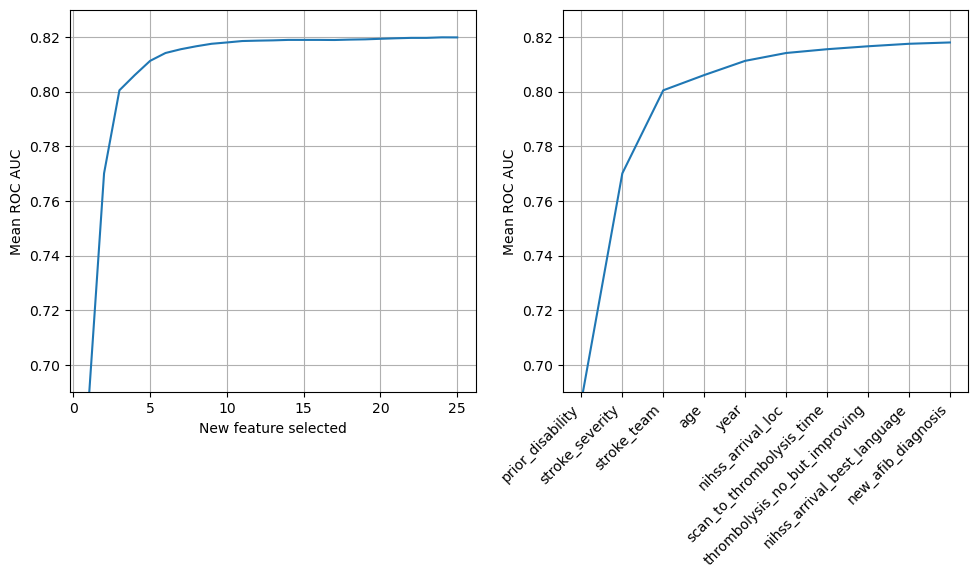
\includegraphics[width=0.75\textwidth]{./images/020_feature_selection.jpg}\\
    \caption{Feature selection}
    \label{fig:feature_selection}
\end{figure}


\subsection{Feature selection}

\textbf{Summary of findings}

Model with all features
The model performance with all 58 features is:
* AUC: 0.818 (std across 5 kfolds: 0.001)
* Accuracy: 0.440 (std across 5 kfolds: 0.002)
* Accuracy within one: 0.760 (std across 5 kfolds: 0.002)

\textbf{Sequentially selecting features}
Sequentially chose features up to 25 features. We saw that once 14 features we selected, the model choose a feature (infarction) that is the same value for all patients, hence no more information was being obtained beyond this point:
Feature  1: prior\_disability, AUC: 0.687
Feature  2: stroke\_severity, AUC: 0.770
Feature  3: stroke\_team, AUC: 0.800
Feature  4: age, AUC: 0.806
Feature  5: year, AUC: 0.811
Feature  6: nihss\_arrival\_loc, AUC: 0.814
Feature  7: scan\_to\_thrombolysis\_time, AUC: 0.816
Feature  8: thrombolysis\_no\_but\_improving, AUC: 0.817
Feature  9: nihss\_arrival\_best\_language, AUC: 0.818
Feature 10: new\_afib\_diagnosis, AUC: 0.818
Feature 11: nihss\_arrival\_sensory, AUC: 0.819
Feature 12: atrial\_fibrillation, AUC: 0.819
Feature 13: nihss\_arrival\_facial\_palsy, AUC: 0.819
Feature 14: thrombolysis\_no\_but\_other\_medical, AUC: 0.819
Feature 15: infarction, AUC: 0.819
Feature 16: arrive\_by\_ambulance, AUC: 0.819
Feature 17: nihss\_arrival\_motor\_arm\_left, AUC: 0.819
Feature 18: thrombolysis\_no\_but\_comorbidity, AUC: 0.819
Feature 19: nihss\_arrival\_loc\_questions, AUC: 0.819
Feature 20: nihss\_arrival\_motor\_arm\_right, AUC: 0.819
Feature 21: nihss\_arrival\_best\_gaze, AUC: 0.820
Feature 22: thrombolysis\_no\_but\_too\_mild\_severe, AUC: 0.820
Feature 23: diabetes, AUC: 0.820
Feature 24: thrombolysis\_no\_but\_haemorrhagic, AUC: 0.820
Feature 25: thrombolysis\_no\_but\_medication, AUC: 0.820

\textbf{Features chosen for the predictive model}
We will include these 7 features in our model (reasoning given below):
Feature  1: prior\_disability
Feature  2: stroke\_severity
Feature  3: stroke\_team
Feature  4: age
Feature  5: onset\_to\_thrombolysis\_time
Feature  6: any\_afib\_diagnosis
Feature  7: precise\_onset\_known

\textbf{Additional experiments to inform choice of features}

To inform us further about which features to include in our model, we carried out some additional experiments (in other notebooks). Here is what we learnt, and our feature selection choice based on this.

\textbf{Why we chose these 7 features:}
* prior\_disability (easy selection choice)
* stroke\_severity (checked the impact of using the separate NIHSS features instead - decided including stroke severity captured the information)
* stroke\_team (easy selection choice)
* age (easy selection choice)
* onset\_to\_thrombolysis\_time (scan\_to\_thrombolysis\_time is a selected feature, however the feature onset-to-thrombolysis time is a more useful feature to include as it aligns with other research and the clinical focus.We compared the SHAP plots from models that included either (and neither) of these duration features. Across the three models, the other features (age, prior disability, stroke severity) are not affected by the inclusion of either duration feature, nor is any performance accuracy lost)
* any\_afib\_diagnosis (Both new\_afib\_diagnosis and atrial\_fibrillation featrures are in the list above, and we have seen that an atrial fibrillation diagnosis contributes for the mRS6 outcome. We will include any\_afib\_diagnosis as this includes both of the other atrial fibrillation features information. We compared the SHAP plots from models that included one of these atrial fibrillation diagnosis features (and none). Across those models, the other features (age, prior disability, stroke severity) are not affected by the inclusion of which atrial fibrillation feature, nor is any performance accuracy lost).
* precise\_onset\_known (Not included in the feature selection list, however may be useful to include so people can see whether it makes a significant difference to outcomes, as this is often a discussion point amongst clinicians)

\textbf{Why we didn't include these features:}
* YEAR: Any data from beyond 2021 (the latest year in the dataset), the model has yet to see any information about that year. If the decision tree treats the ”Year” feature as a numerical value, any future year will be grouped along with year 2021 for each split - check how the model is treating the Year feature.

We reran feature selection excluding the feature "stroke team" as an option. The feature "Year" was now not a selected features. Here are those results:

There are 56 features
All features, AUC: 0.786 (std across 5 kfolds: 0.001)
All features, accuracy: 0.387 (std across 5 kfolds: 0.003)
All features, accuracy within one: 0.734 (std across 5 kfolds: 0.003)

Feature  1: prior\_disability, AUC: 0.687
Feature  2: stroke\_severity, AUC: 0.770
Feature  3: age, AUC: 0.777
Feature  4: nihss\_arrival\_loc, AUC: 0.779
Feature  5: scan\_to\_thrombolysis\_time, AUC: 0.780
Feature  6: thrombolysis\_no\_but\_improving, AUC: 0.782
Feature  7: nihss\_arrival\_best\_language, AUC: 0.783
Feature  8: thrombolysis\_no\_but\_other\_medical, AUC: 0.783
Feature  9: nihss\_arrival\_sensory, AUC: 0.784
Feature 10: nihss\_arrival\_facial\_palsy, AUC: 0.784
Feature 11: nihss\_arrival\_limb\_ataxia, AUC: 0.784
Feature 12: nihss\_arrival\_motor\_arm\_left, AUC: 0.785
Feature 13: nihss\_arrival\_best\_gaze, AUC: 0.785
Feature 14: diabetes, AUC: 0.785
Feature 15: thrombolysis\_no\_but\_comorbidity, AUC: 0.785
Feature 16: nihss\_arrival\_motor\_arm\_right, AUC: 0.786
Feature 17: thrombolysis\_no\_but\_too\_mild\_severe, AUC: 0.786
Feature 18: onset\_during\_sleep, AUC: 0.786
Feature 19: precise\_onset\_known, AUC: 0.786
Feature 20: atrial\_fibrillation, AUC: 0.786
Feature 21: infarction, AUC: 0.786
Feature 22: arrive\_by\_ambulance, AUC: 0.786
Feature 23: nihss\_complete, AUC: 0.786
Feature 24: prior\_stroke\_tia, AUC: 0.786
Feature 25: nihss\_arrival\_dysarthria, AUC: 0.786

To investigate the interaction between "stroke team" and "year" we created some binary models (as SHAP interaction can not be calculated for a multiclass model). This showed that ....

* Individual NIHSS features are not included, as we are already including the feature stroke severity, and this is dependent on the individual NIHSS features (SHAP required features to be independant, apart from with the target feature)
* scan\_to\_thrombolysis\_time is being represented by the feature onset\_to\_thrombolysis\_time
* atrial\_fibrillation and new\_afib\_dianosis are being represented by the feature any\_afib\_diagnosis
* thrombolysis\_no\_but\_improving (there is a messiness of this feature overlapping with the onset\_to\_thrombolysis\_time. We would now have two features saying that the patient does not receive IVT).
* thrombolysis\_no\_but\_other\_medical (the SHAP plots show that this feature does not have a big effect on predicting the outcome).

\iffalse
\subsection{Learning curve}


\begin{figure}[!ht]
\centering
    \subfloat[]{\includegraphics[width=0.5\linewidth]{./images/015_xgb_all_features_learning_curve_binary_learning_curve_mrs0.jpg}}
\hfil
    \subfloat[]{\includegraphics[width=0.5\linewidth]{./images/015_xgb_all_features_learning_curve_binary_learning_curve_mrs1.jpg}}

    \subfloat[]{\includegraphics[width=0.5\linewidth]{./images/015_xgb_all_features_learning_curve_binary_learning_curve_mrs2.jpg}}
\hfil
    \subfloat[]{\includegraphics[width=0.5\linewidth]{./images/015_xgb_all_features_learning_curve_binary_learning_curve_mrs3.jpg}}

    \subfloat[]{\includegraphics[width=0.5\linewidth]{./images/015_xgb_all_features_learning_curve_binary_learning_curve_mrs4.jpg}}
\hfil
    \subfloat[]{\includegraphics[width=0.5\linewidth]{./images/015_xgb_all_features_learning_curve_binary_learning_curve_mrs5.jpg}}
    \label{fig:learning_rate}
  \caption{Learning rate for each of the mRS threshold levels to define a good outcome (using all the data). Model has all input features.}

\end{figure}
\fi


\subsection{Effect of choosing 7 features on accuracy}


\begin{figure}[!ht]
    \centering
        \begin{tabular}{lllll}
        \toprule
         & Model accuracy (\%) & &Accuracy captured (\%)\\ 
%         \midrule
%        \toprule
         mRS range & All features & 7 features & by 7 feature model\\ 
         \midrule
        mRS 0 & 89.9  & 88.2 & 98.1\\
        mRS 0-1 & 81.5  & 77.6 & 95.2\\
        mRS 0-2 & 83.2  & 80.0 & 96.2\\
        mRS 0-3 & 87.1  & 84.3 & 96.8\\
        mRS 0-4 & 90.6  & 88.1 & 97.2\\
        mRS 0-5 & 92.1  & 89.7 & 97.4\\
        \bottomrule
        \end{tabular}
      \caption{Accuracy of model with all 57 features, and 7 features.}
      \label{fig:table_accuracy_feature_selection}

\end{figure}

\begin{figure}[!ht]
    \centering
        \begin{tabular}{lllll}
        \toprule
         & Model ROCAUC (\%) & &ROCAUC captured (\%)\\ 
%         \midrule
%        \toprule
         mRS range & All features & 7 features & by 7 feature model\\ 
         \midrule
        mRS 0 & 90.8  & 85.3 & 93.9\\ 
        mRS 0-1 & 89.4  & 85.2 & 95.3\\
        mRS 0-2 & 91.1  & 87.6 & 96.2\\
        mRS 0-3 & 92.5  & 89.0 & 96.2\\
        mRS 0-4 & 93.5  & 89.3 & 95.5\\
        mRS 0-5 & 92.6  & 86.8 & 93.7\\
        \bottomrule
        \end{tabular}
      \caption{ROC AUC of model with all 57 features, and 7 features.}
      \label{fig:table_rocauc_feature_selection}

\end{figure}

\begin{figure}[!h]
    \centering
    \begin{subfigure}[b]{1\textwidth}
      \centering
      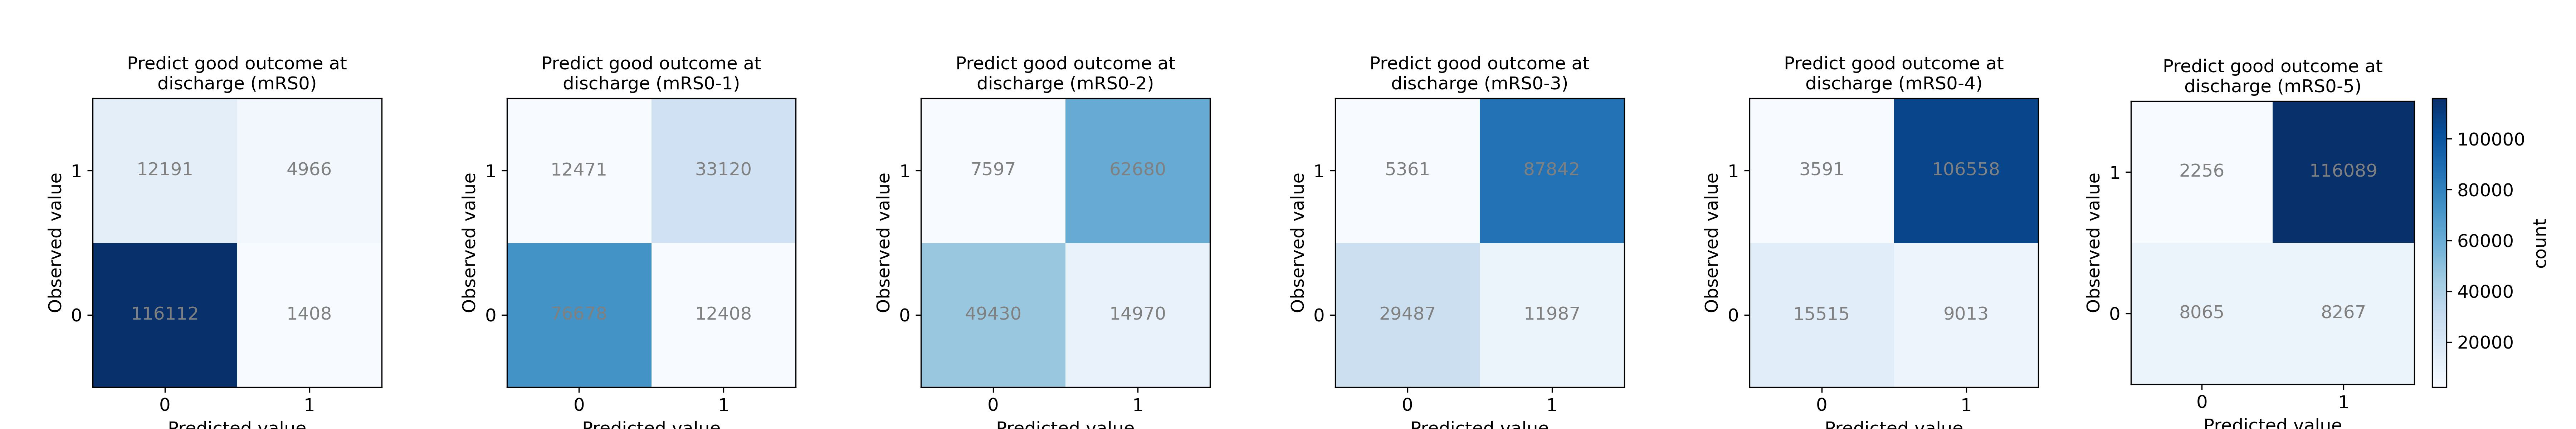
\includegraphics[width=1\textwidth]{./images/073_xgb_all_features_5fold_binary_confusion_matrices_per_binary_threshold_kfold0}\\
      \caption{Kfold 1}
      \label{fig:results_waterfall}
    \end{subfigure}
    \hfill
    \begin{subfigure}[b]{1\textwidth}
      \centering    
      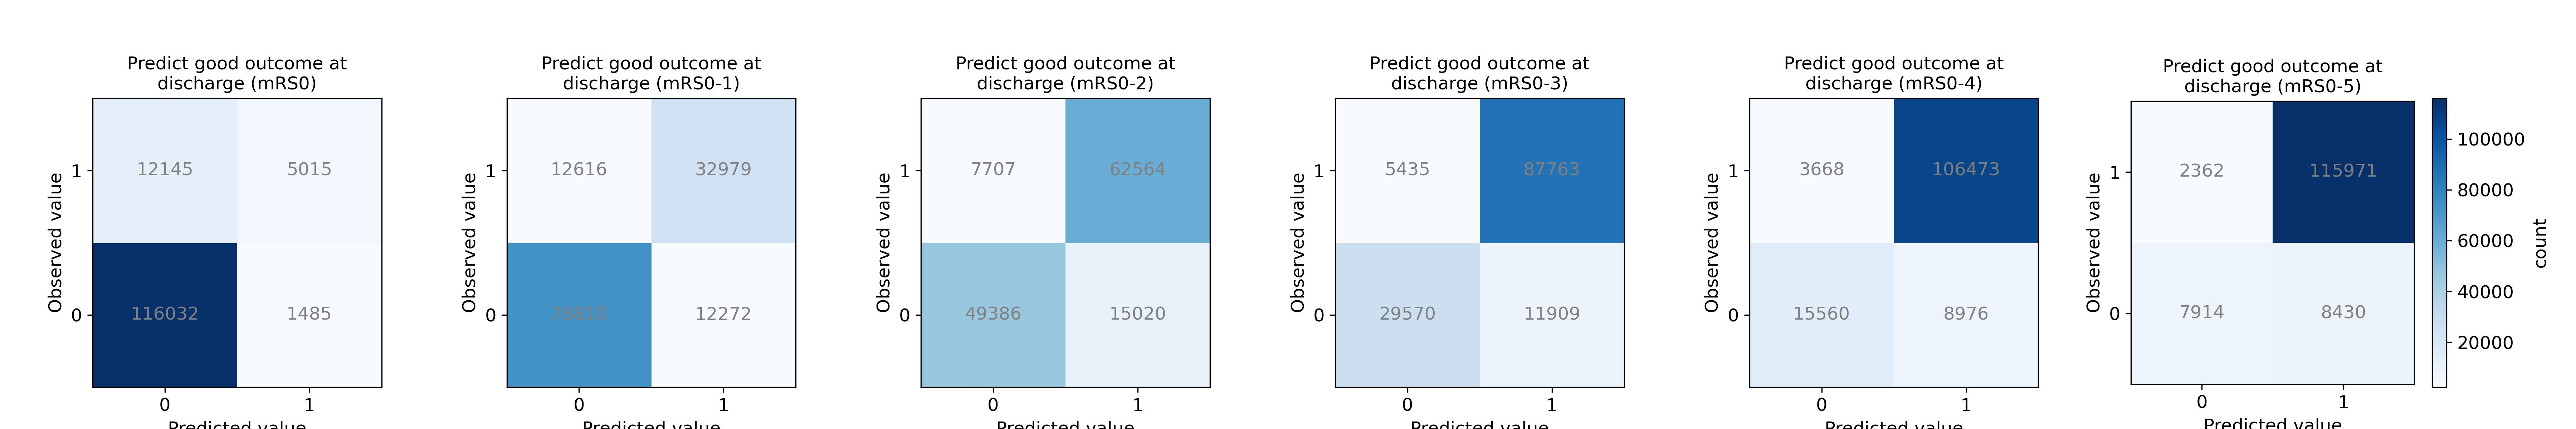
\includegraphics[width=1\textwidth]{./images/073_xgb_all_features_5fold_binary_confusion_matrices_per_binary_threshold_kfold1}\\
      \caption{Kfold 2}
      \label{fig:results_waterfall}
    \end{subfigure}
    \hfill
    \begin{subfigure}[b]{1\textwidth}
      \centering
      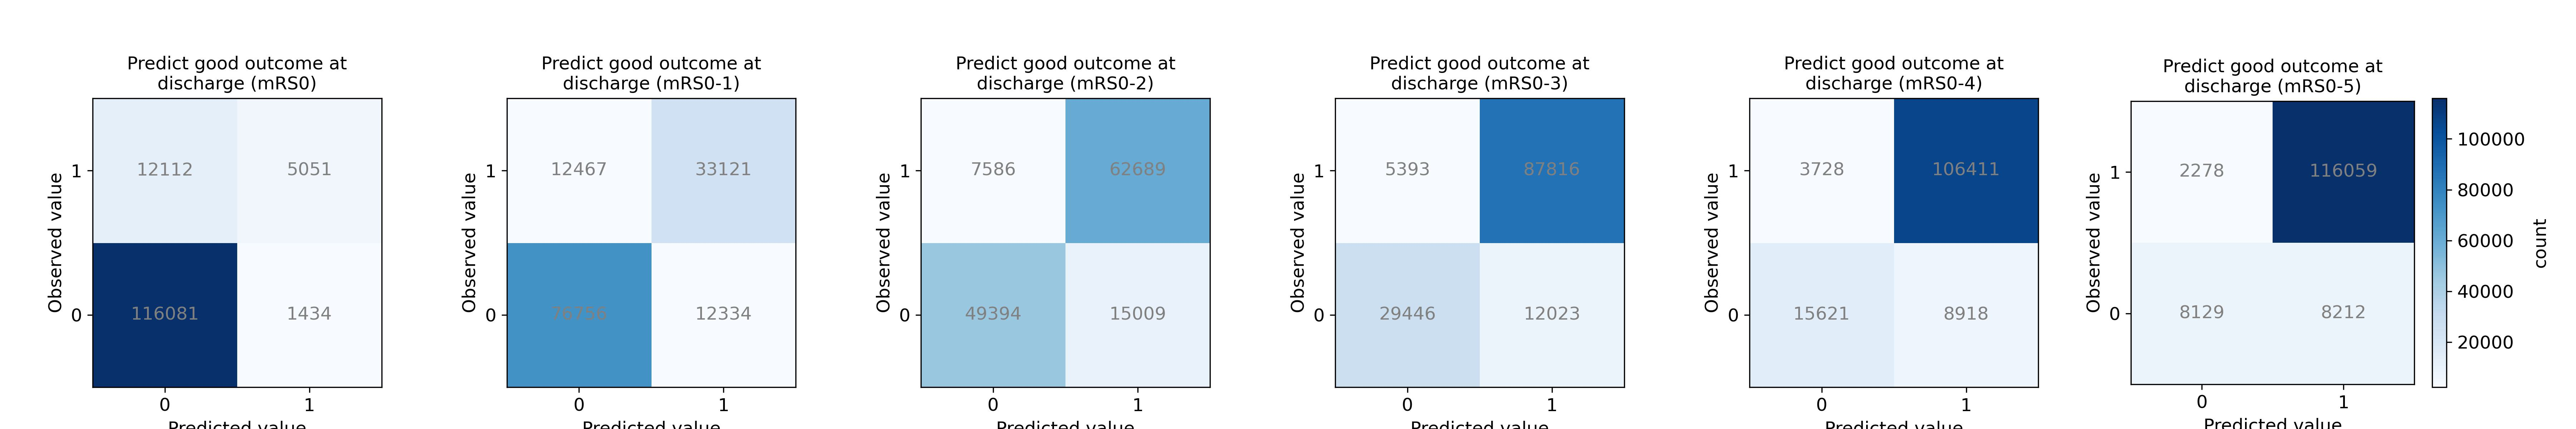
\includegraphics[width=1\textwidth]{./images/073_xgb_all_features_5fold_binary_confusion_matrices_per_binary_threshold_kfold2}\\
      \caption{Kfold 3}
      \label{fig:results_waterfall}
    \end{subfigure}
    \hfill
    \begin{subfigure}[b]{1\textwidth}
      \centering
      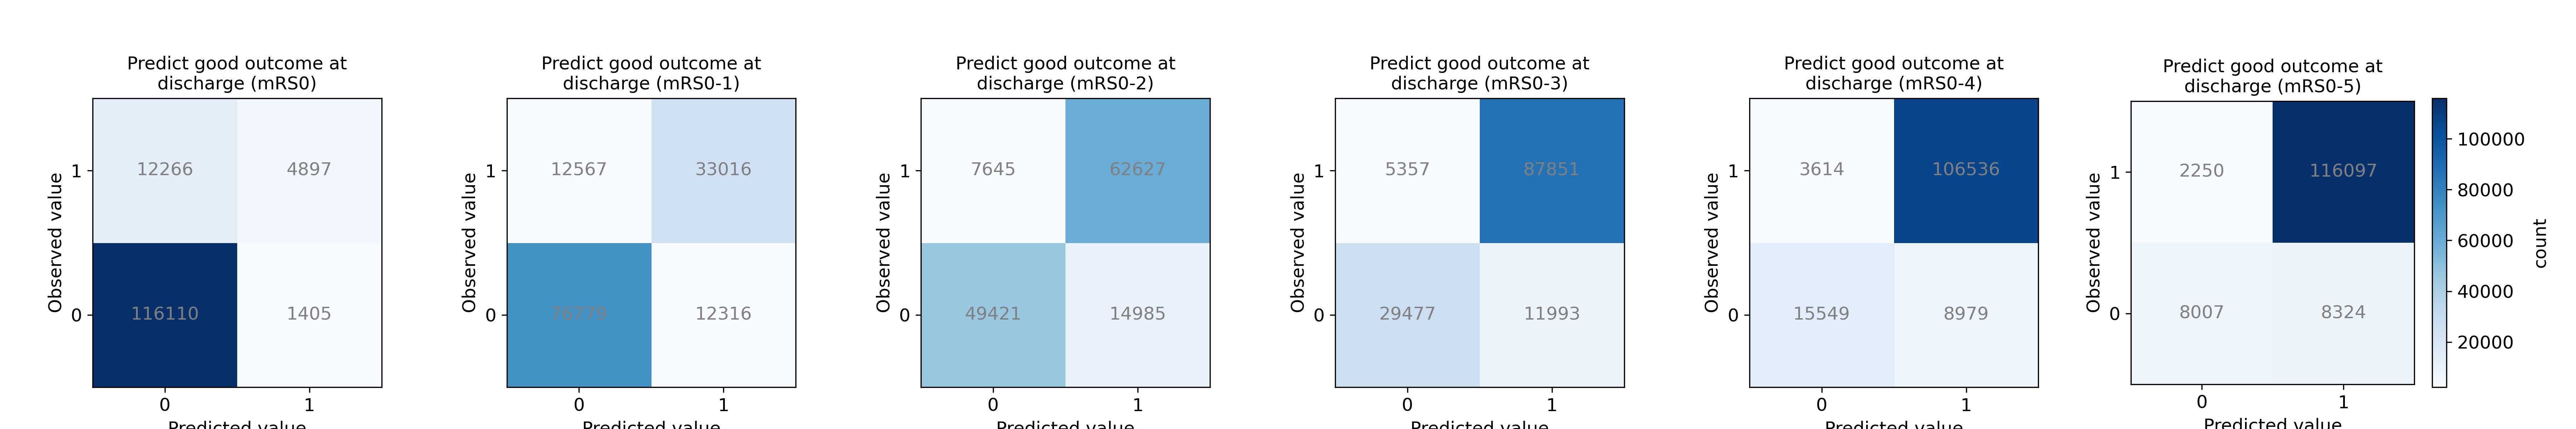
\includegraphics[width=1\textwidth]{./images/073_xgb_all_features_5fold_binary_confusion_matrices_per_binary_threshold_kfold3}\\
      \caption{Kfold 4}
      \label{fig:results_waterfall}
    \end{subfigure}
    \hfill
    \begin{subfigure}[b]{1\textwidth}
      \centering
      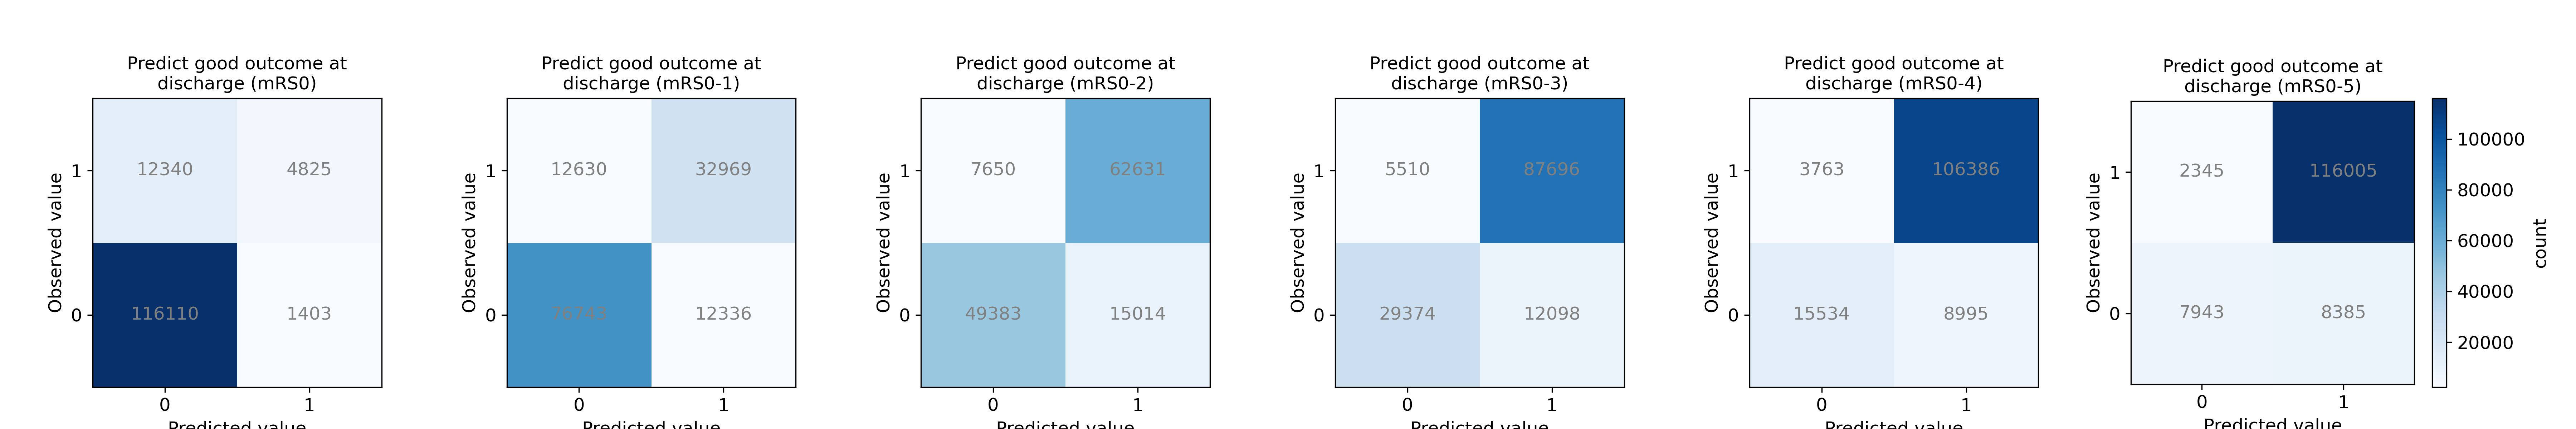
\includegraphics[width=1\textwidth]{./images/073_xgb_all_features_5fold_binary_confusion_matrices_per_binary_threshold_kfold4}\\
      \caption{Kfold 5}
      \label{fig:results_waterfall}
    \end{subfigure}
  \caption{Confusion matrices for each kfold (model with all features)}
\end{figure}

\begin{figure}[!ht]
\centering
    \subfloat[]{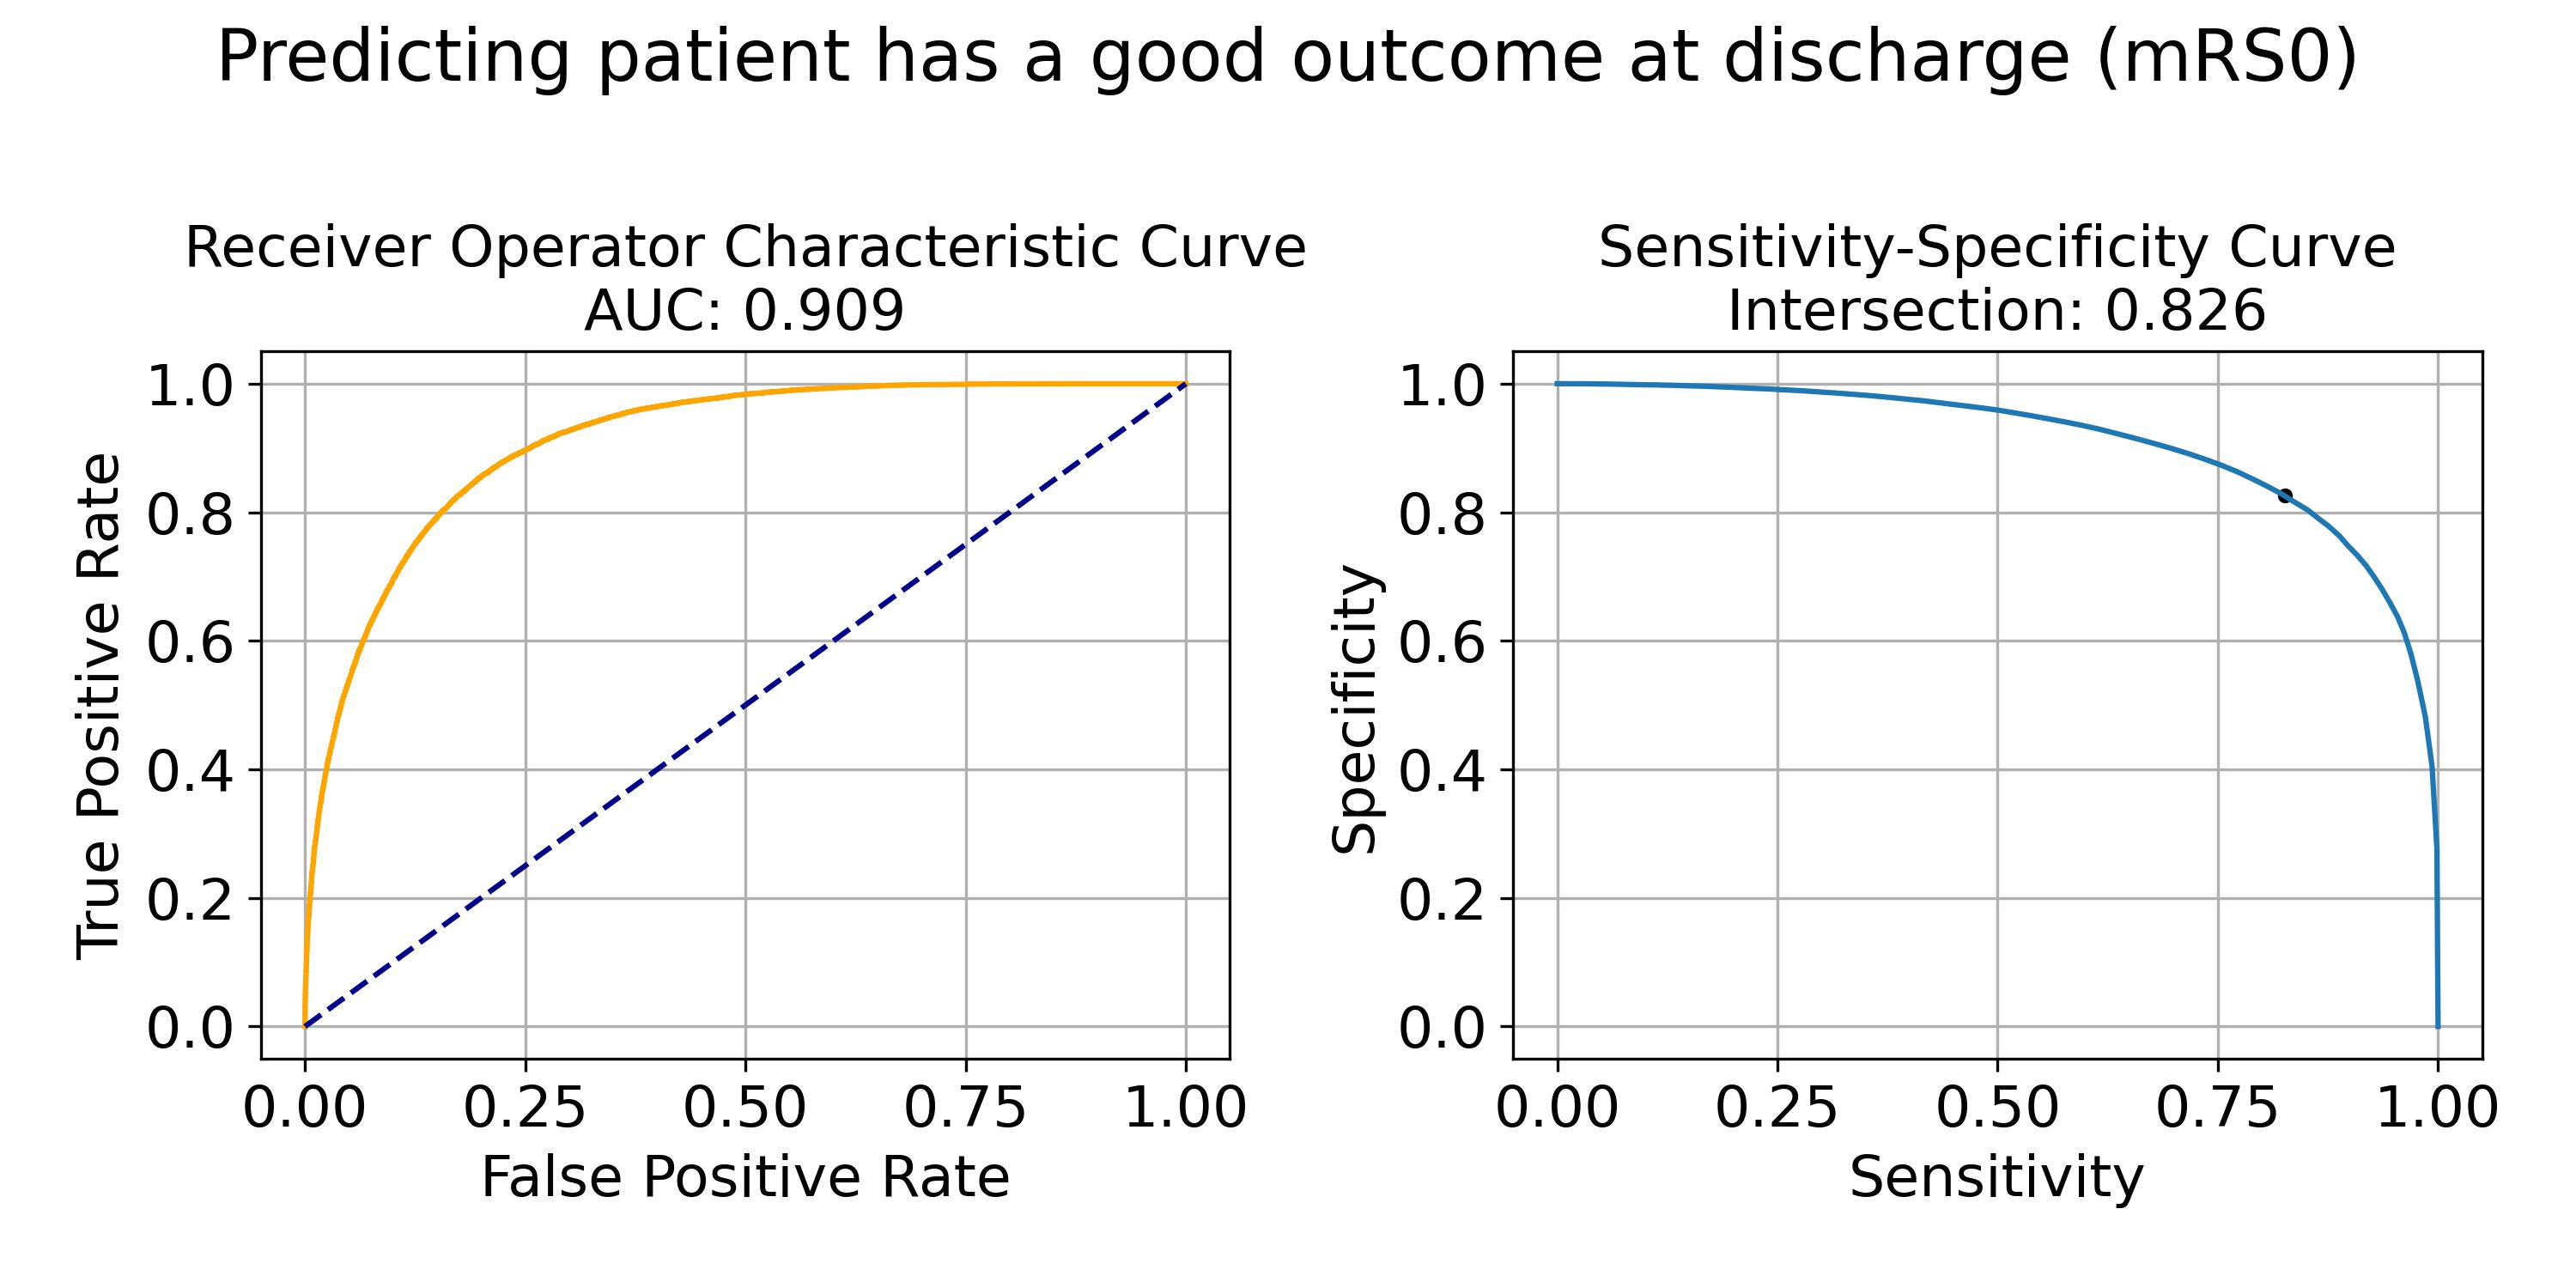
\includegraphics[width=0.5\linewidth]{./images/073_xgb_all_features_5fold_binary_roc_sens_spec_mrs0_kfold0_paper}}
\hfil
    \subfloat[]{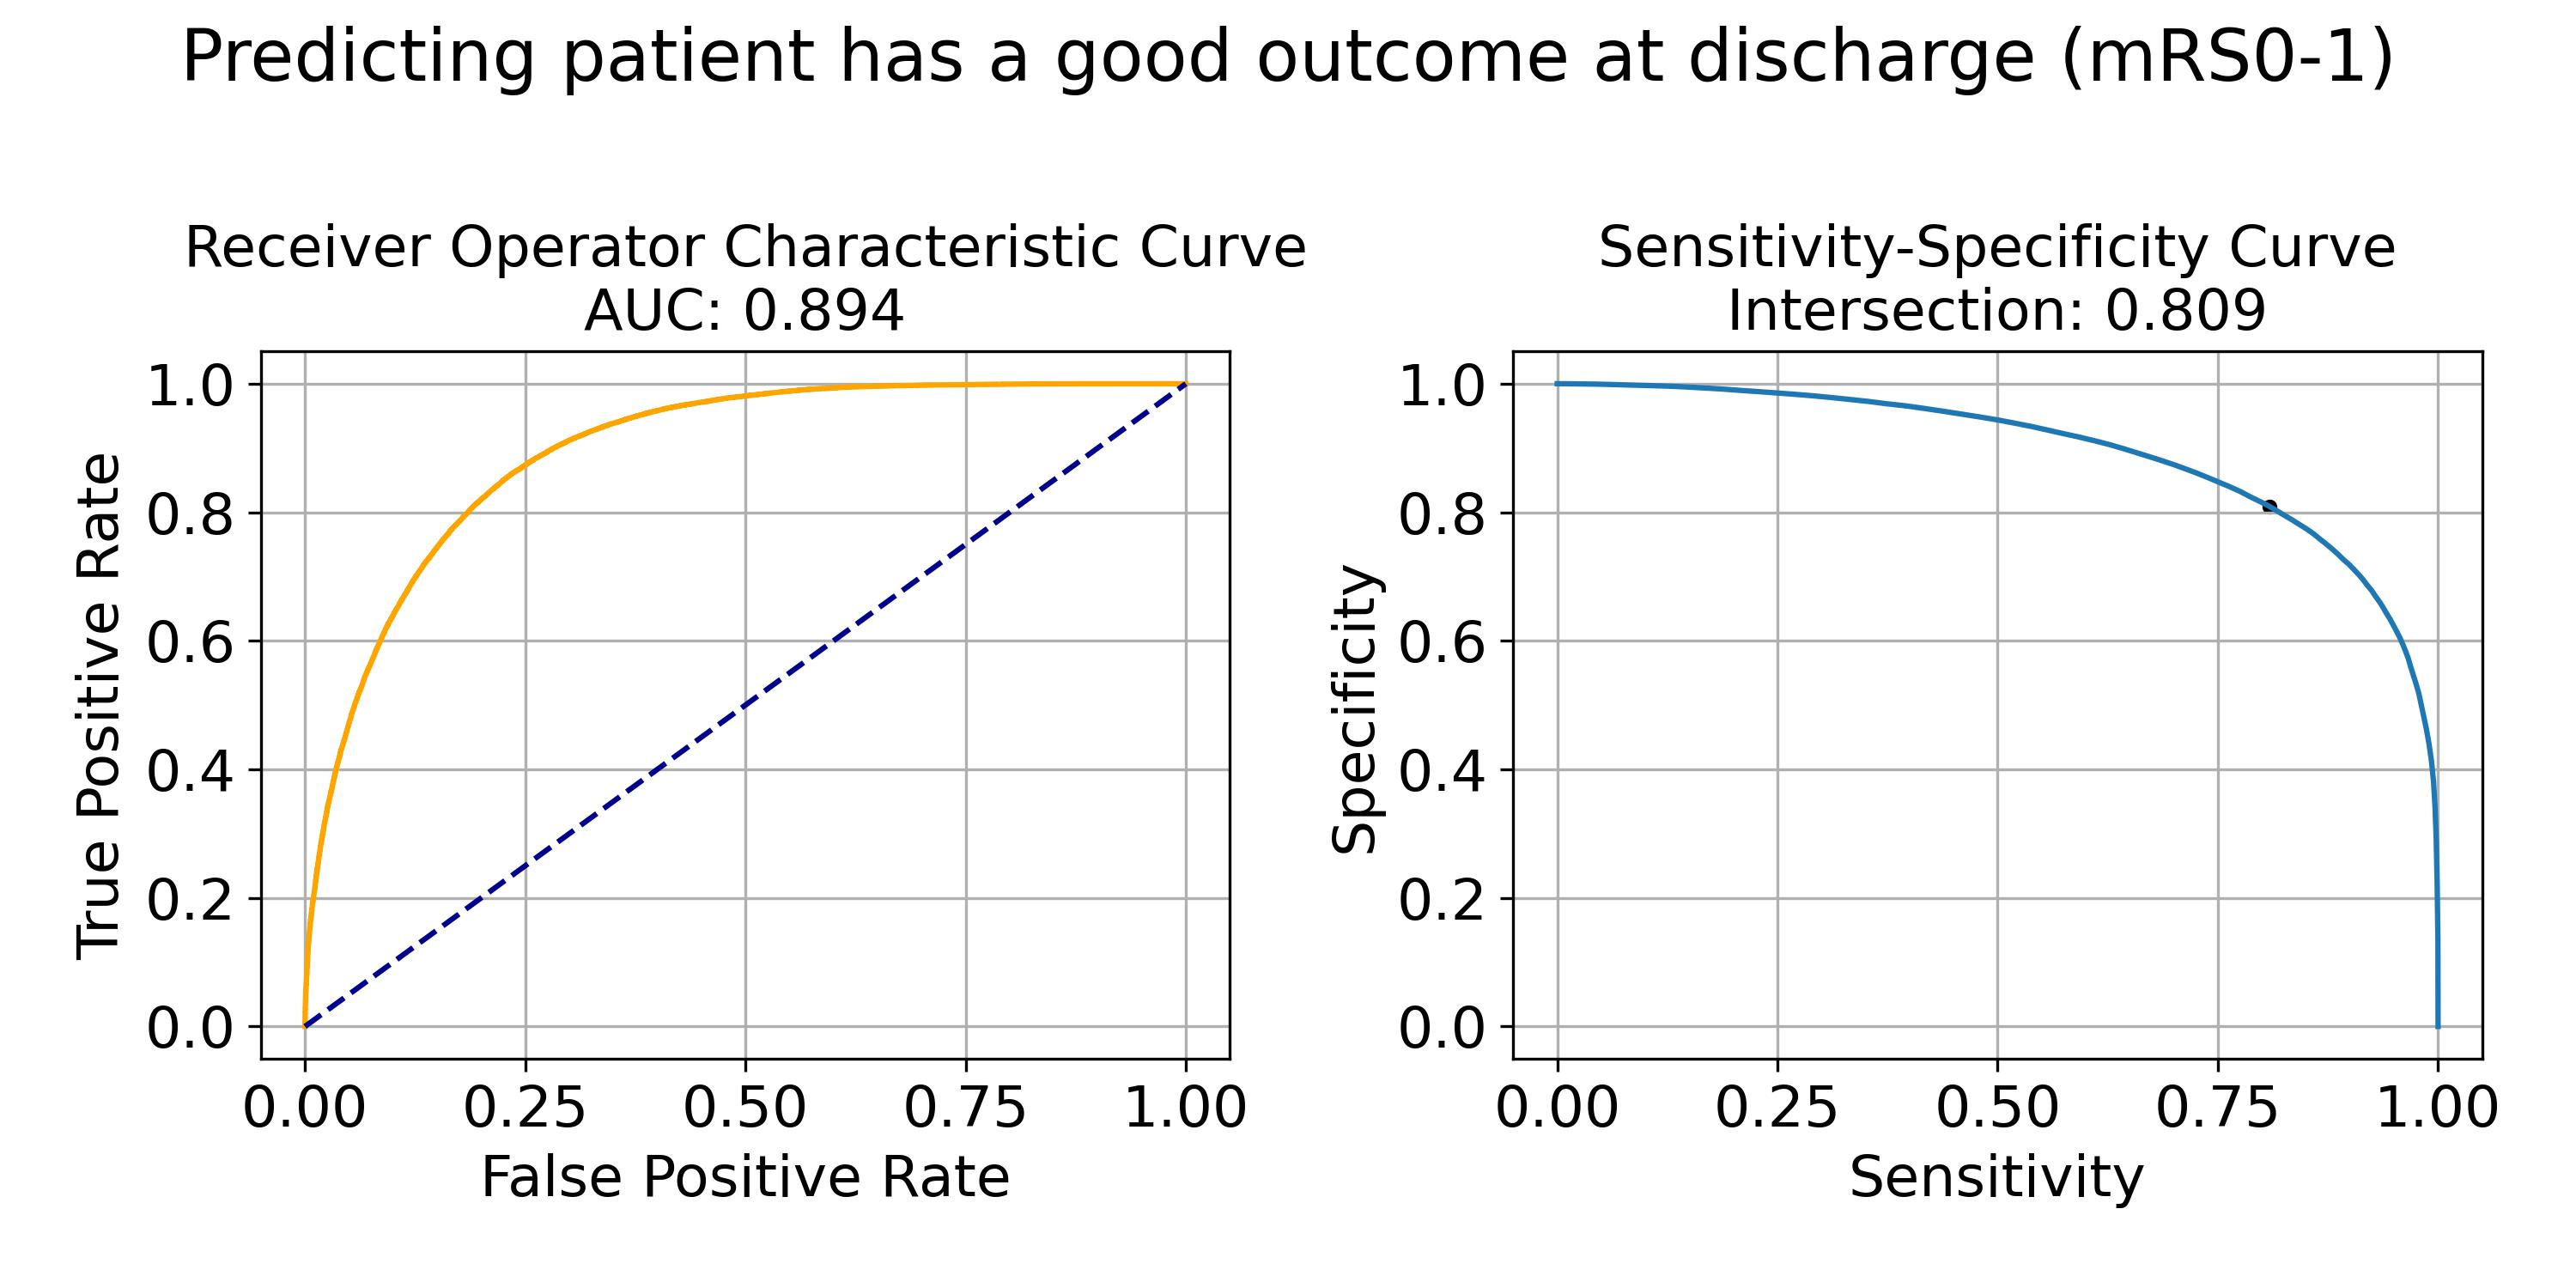
\includegraphics[width=0.5\linewidth]{./images/073_xgb_all_features_5fold_binary_roc_sens_spec_mrs1_kfold0_paper}}

    \subfloat[]{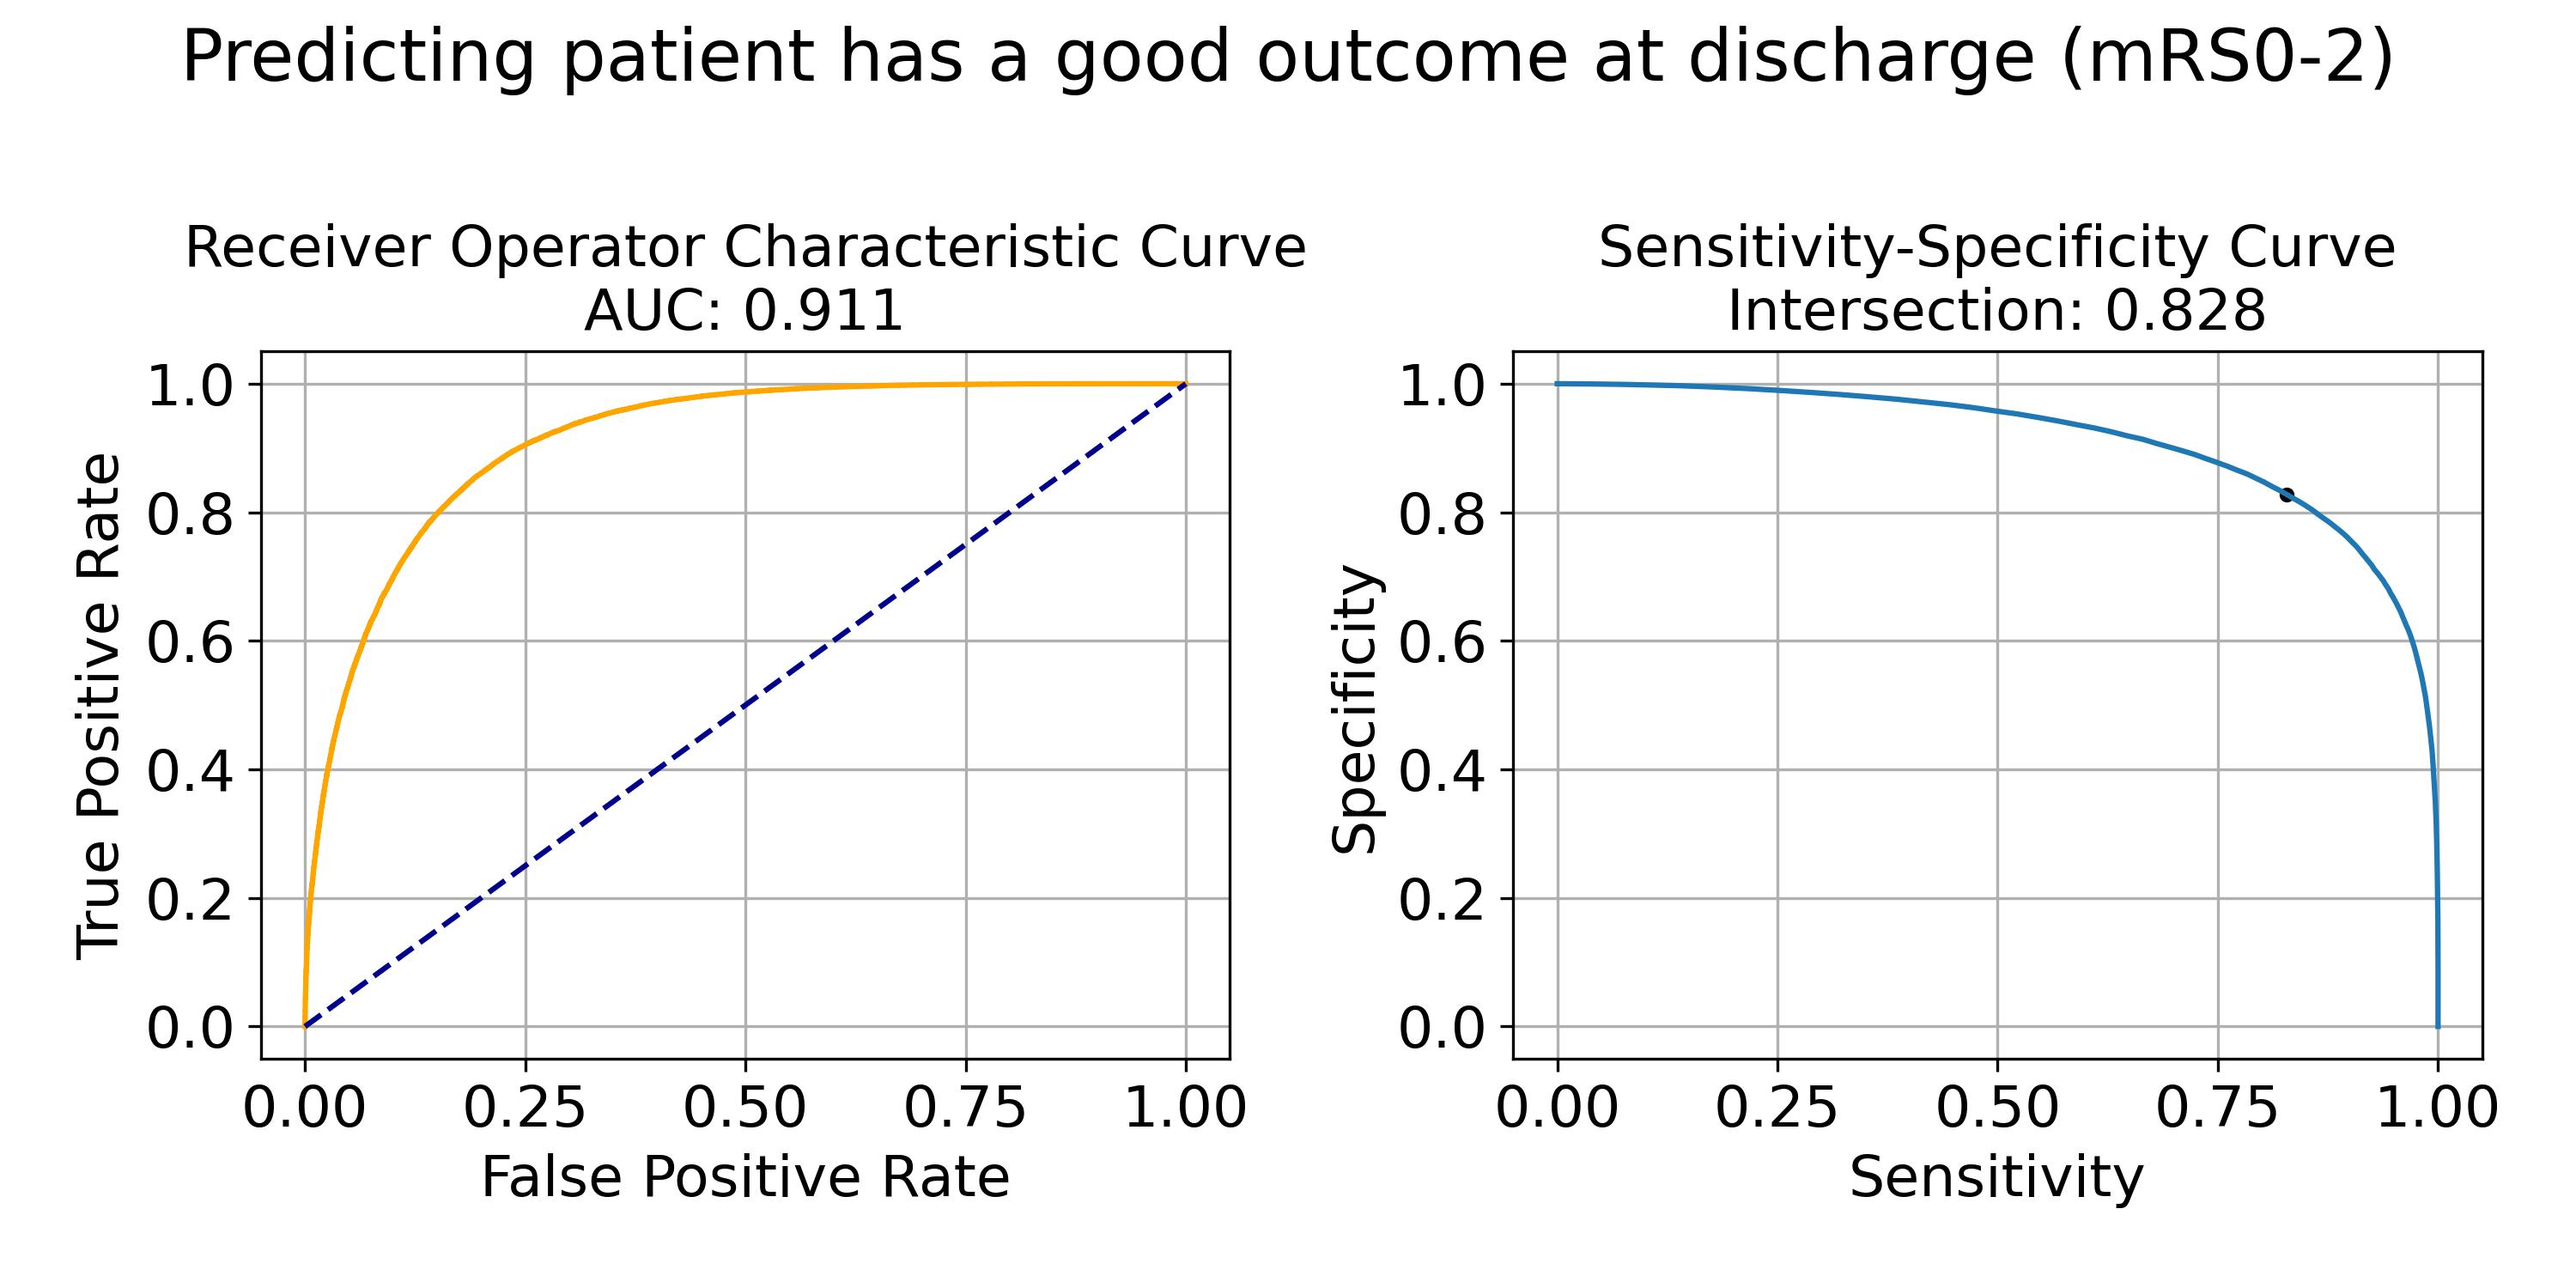
\includegraphics[width=0.5\linewidth]{./images/073_xgb_all_features_5fold_binary_roc_sens_spec_mrs2_kfold0_paper}}
\hfil
    \subfloat[]{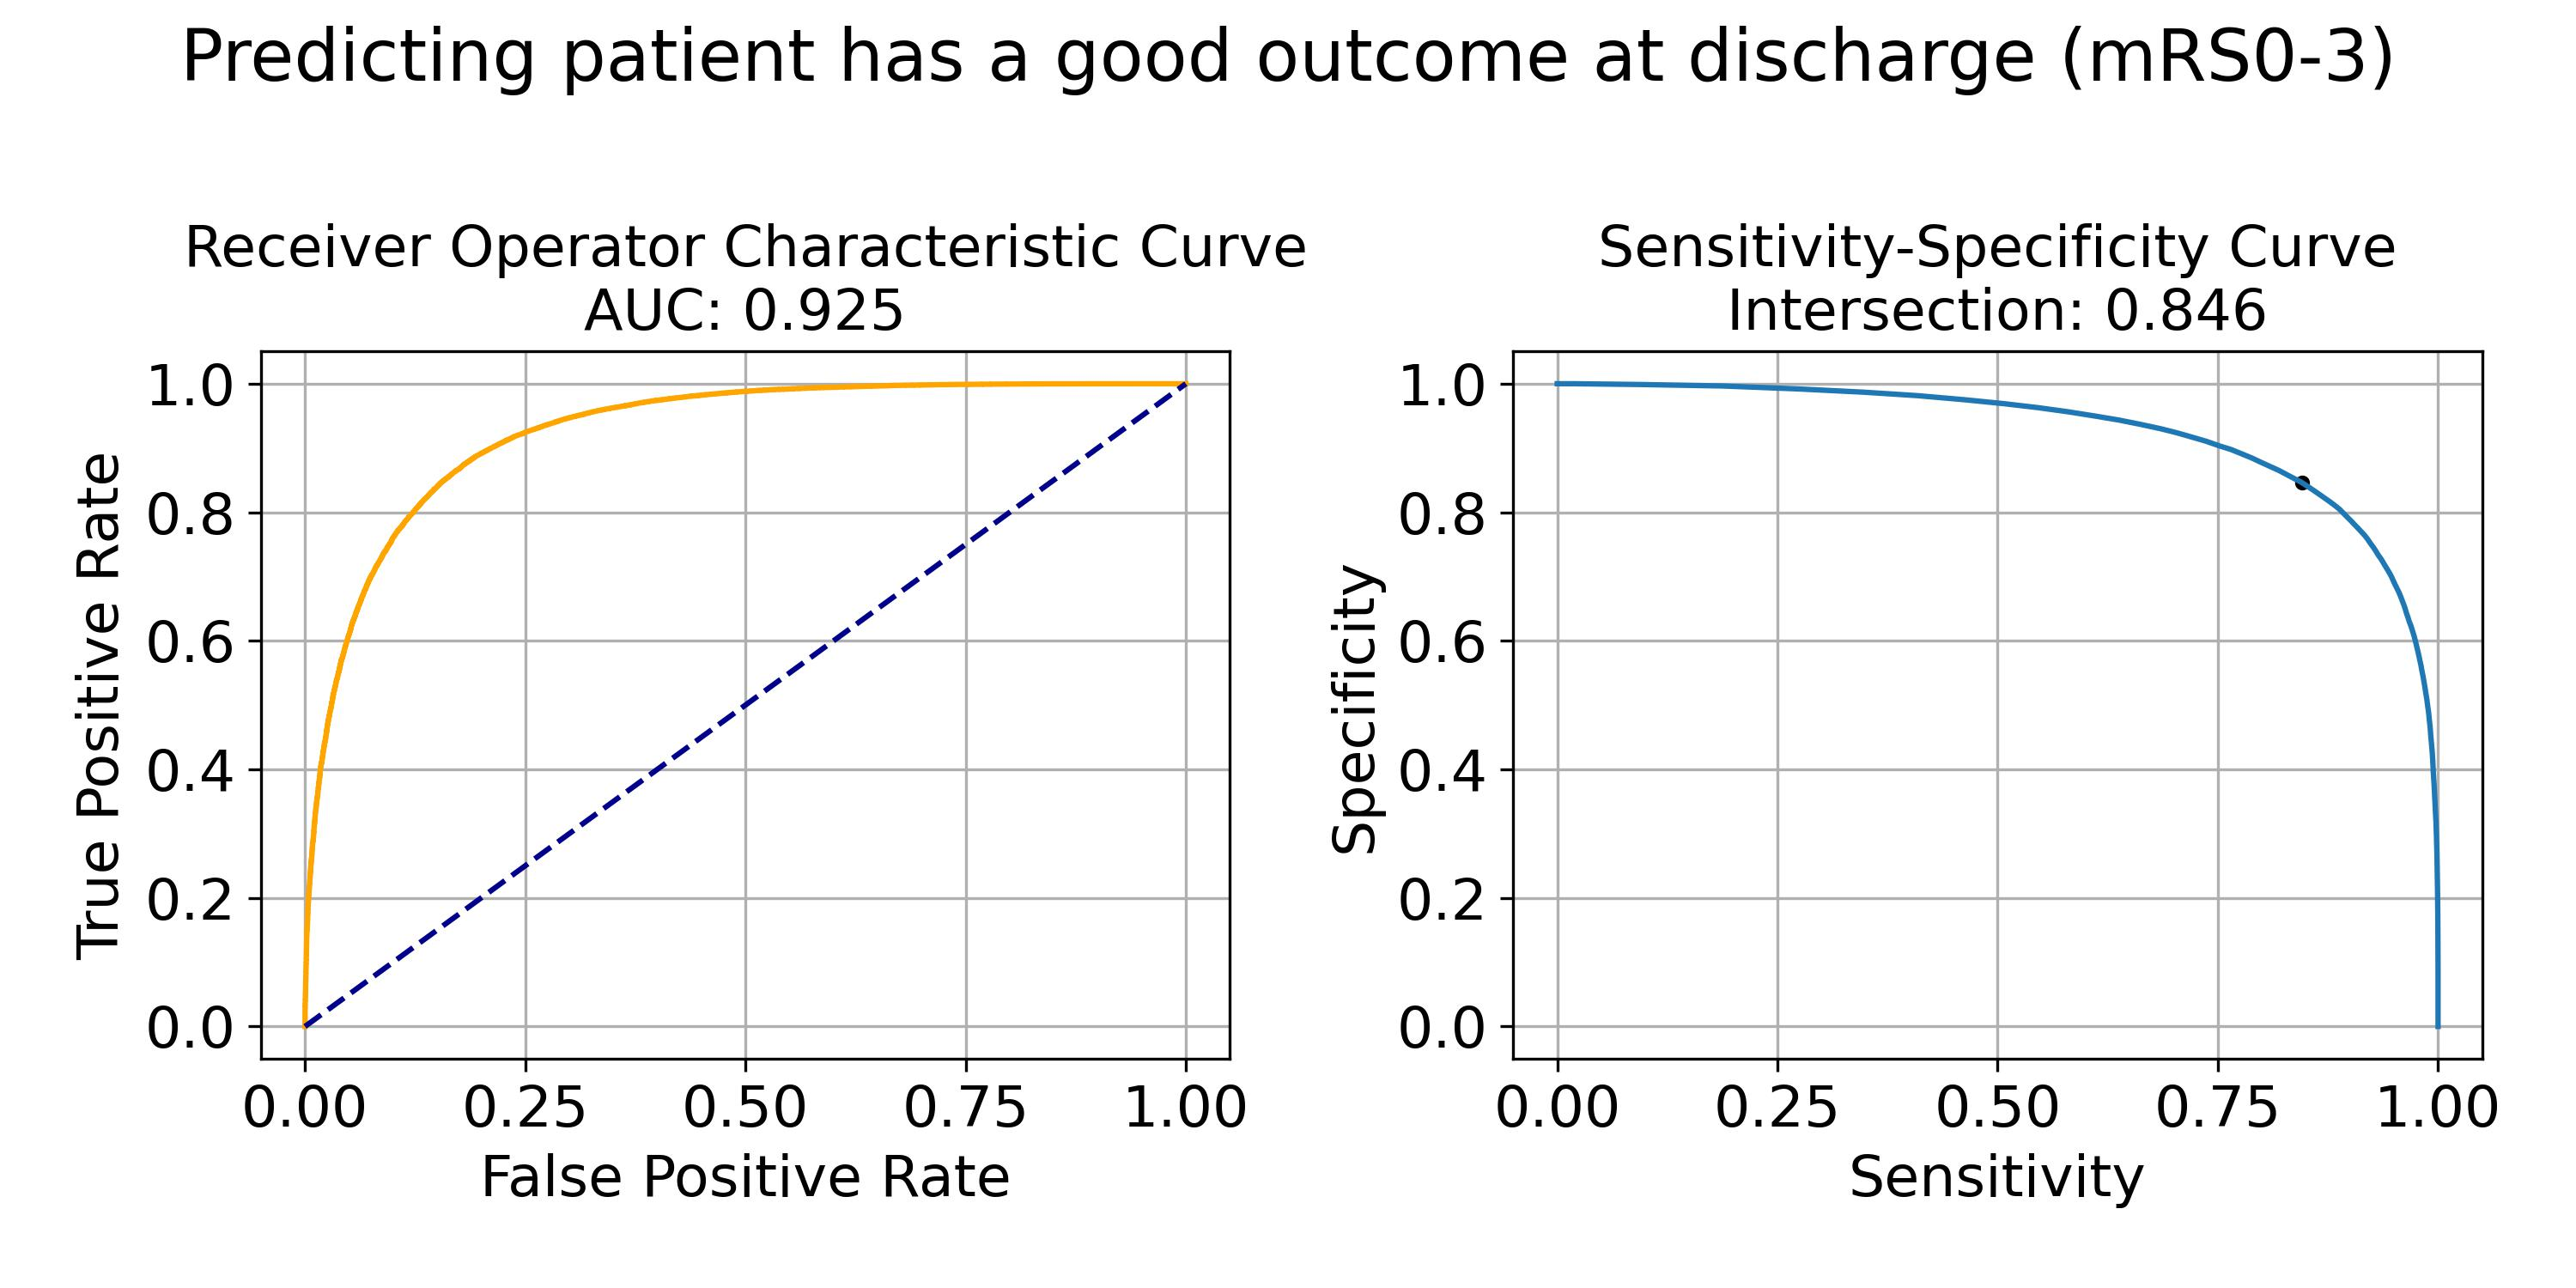
\includegraphics[width=0.5\linewidth]{./images/073_xgb_all_features_5fold_binary_roc_sens_spec_mrs3_kfold0_paper}}

    \subfloat[]{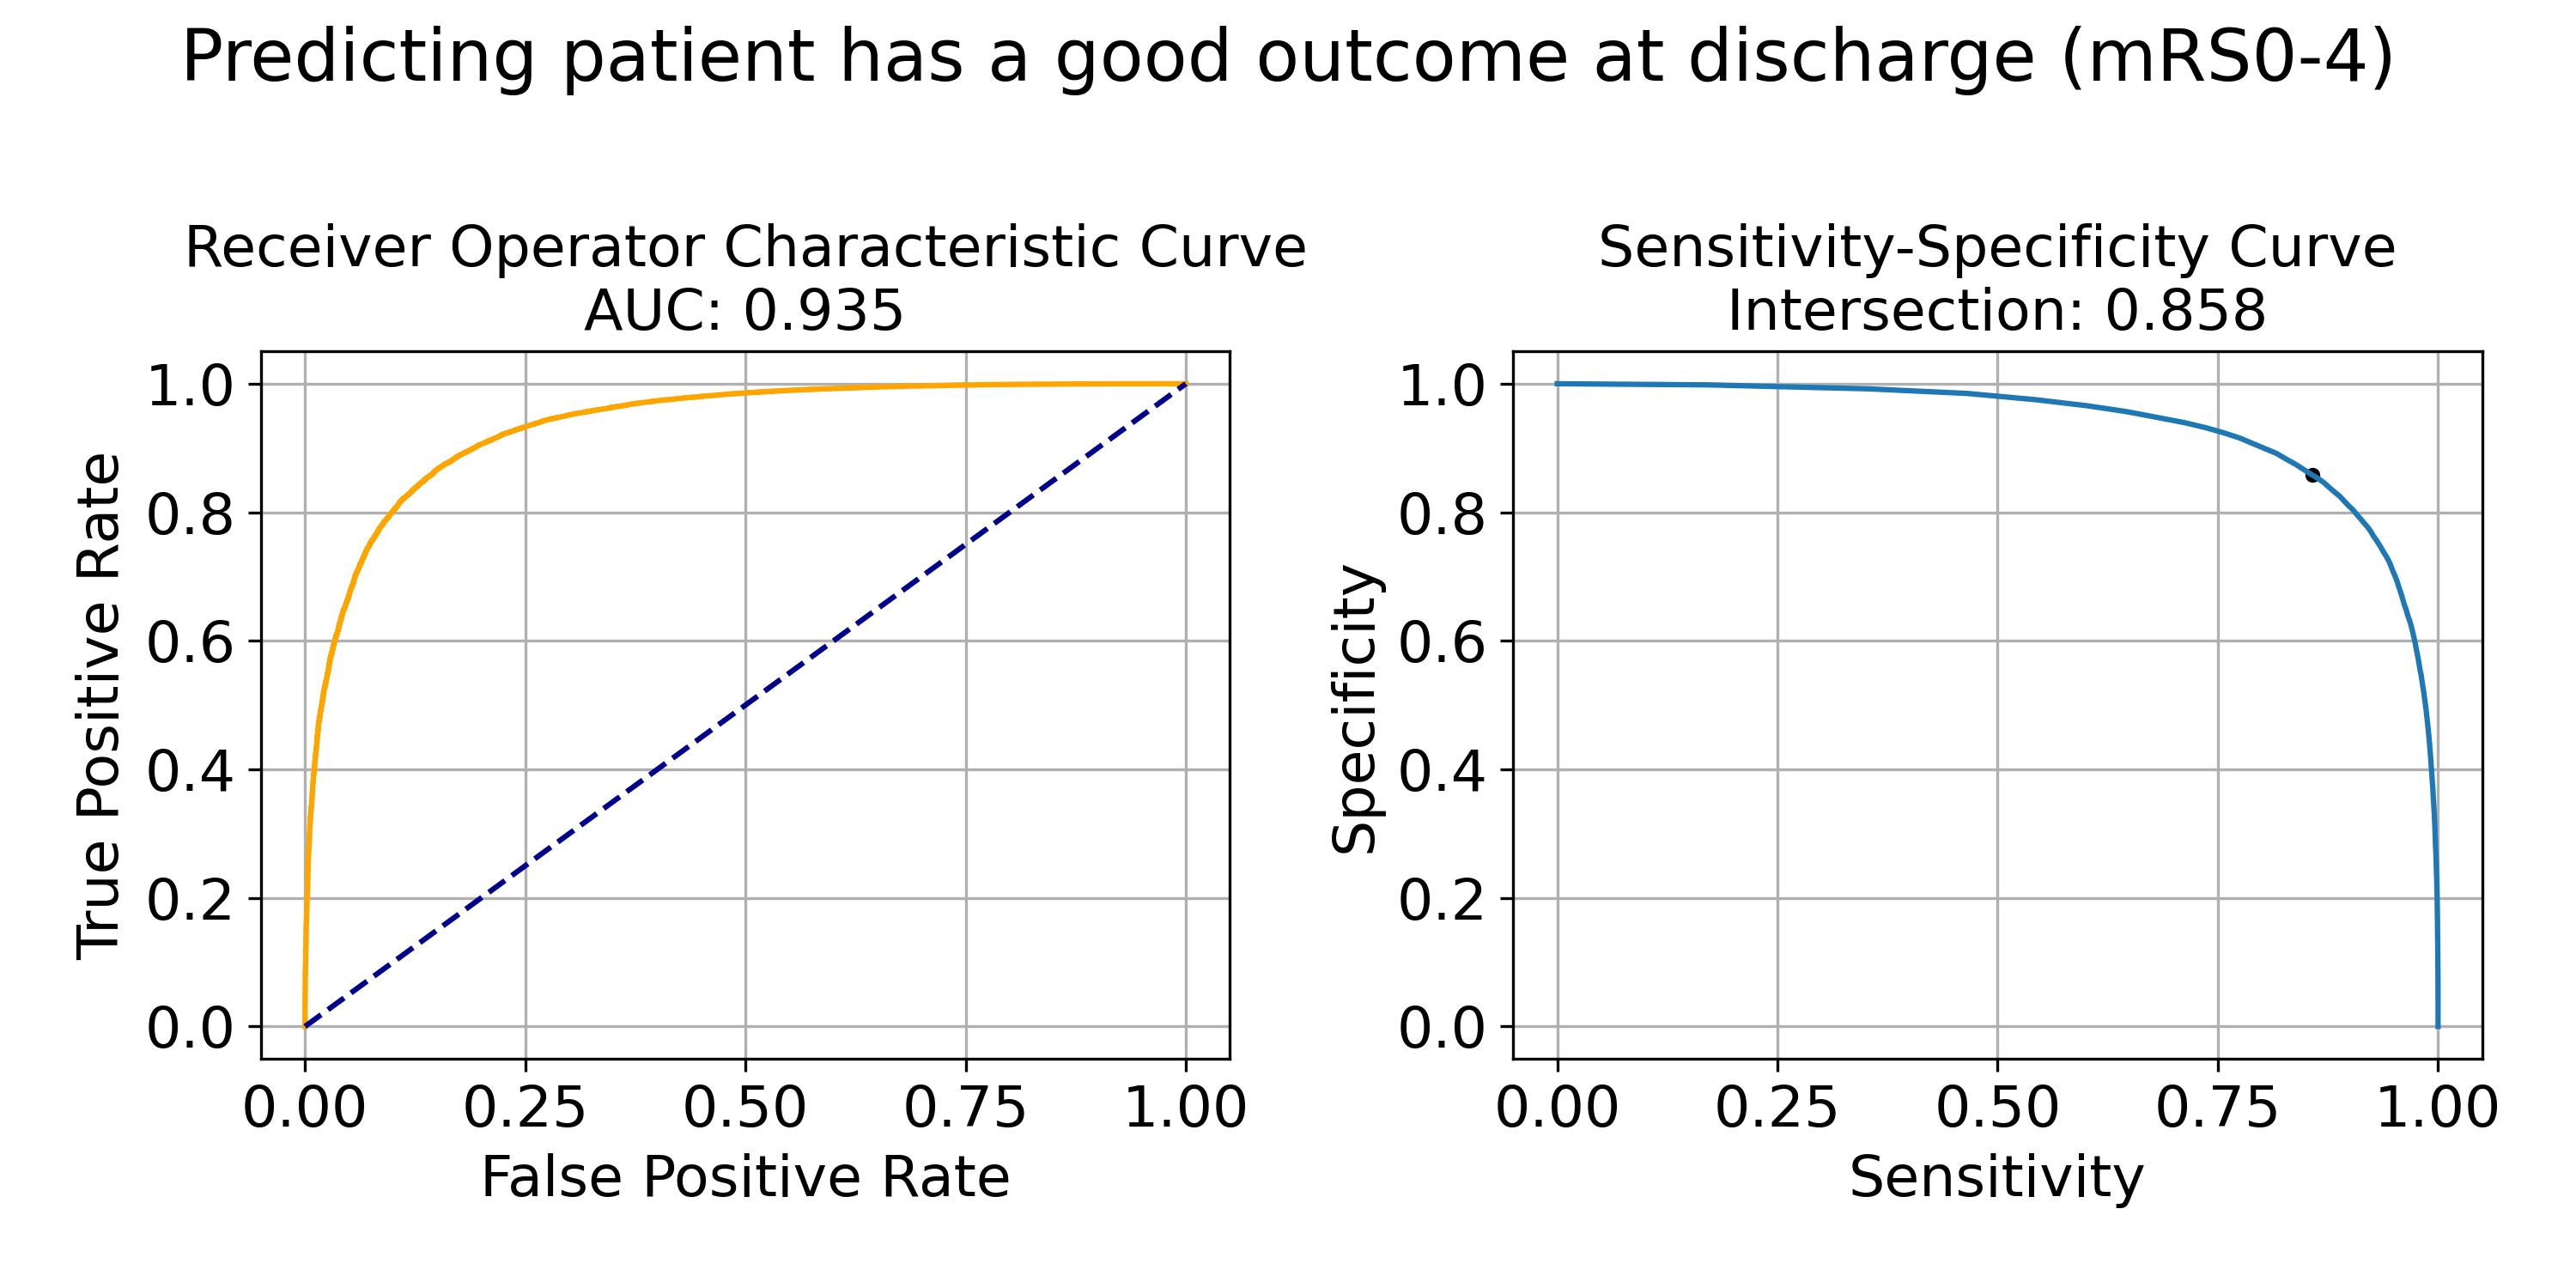
\includegraphics[width=0.5\linewidth]{./images/073_xgb_all_features_5fold_binary_roc_sens_spec_mrs4_kfold0_paper}}
\hfil
    \subfloat[]{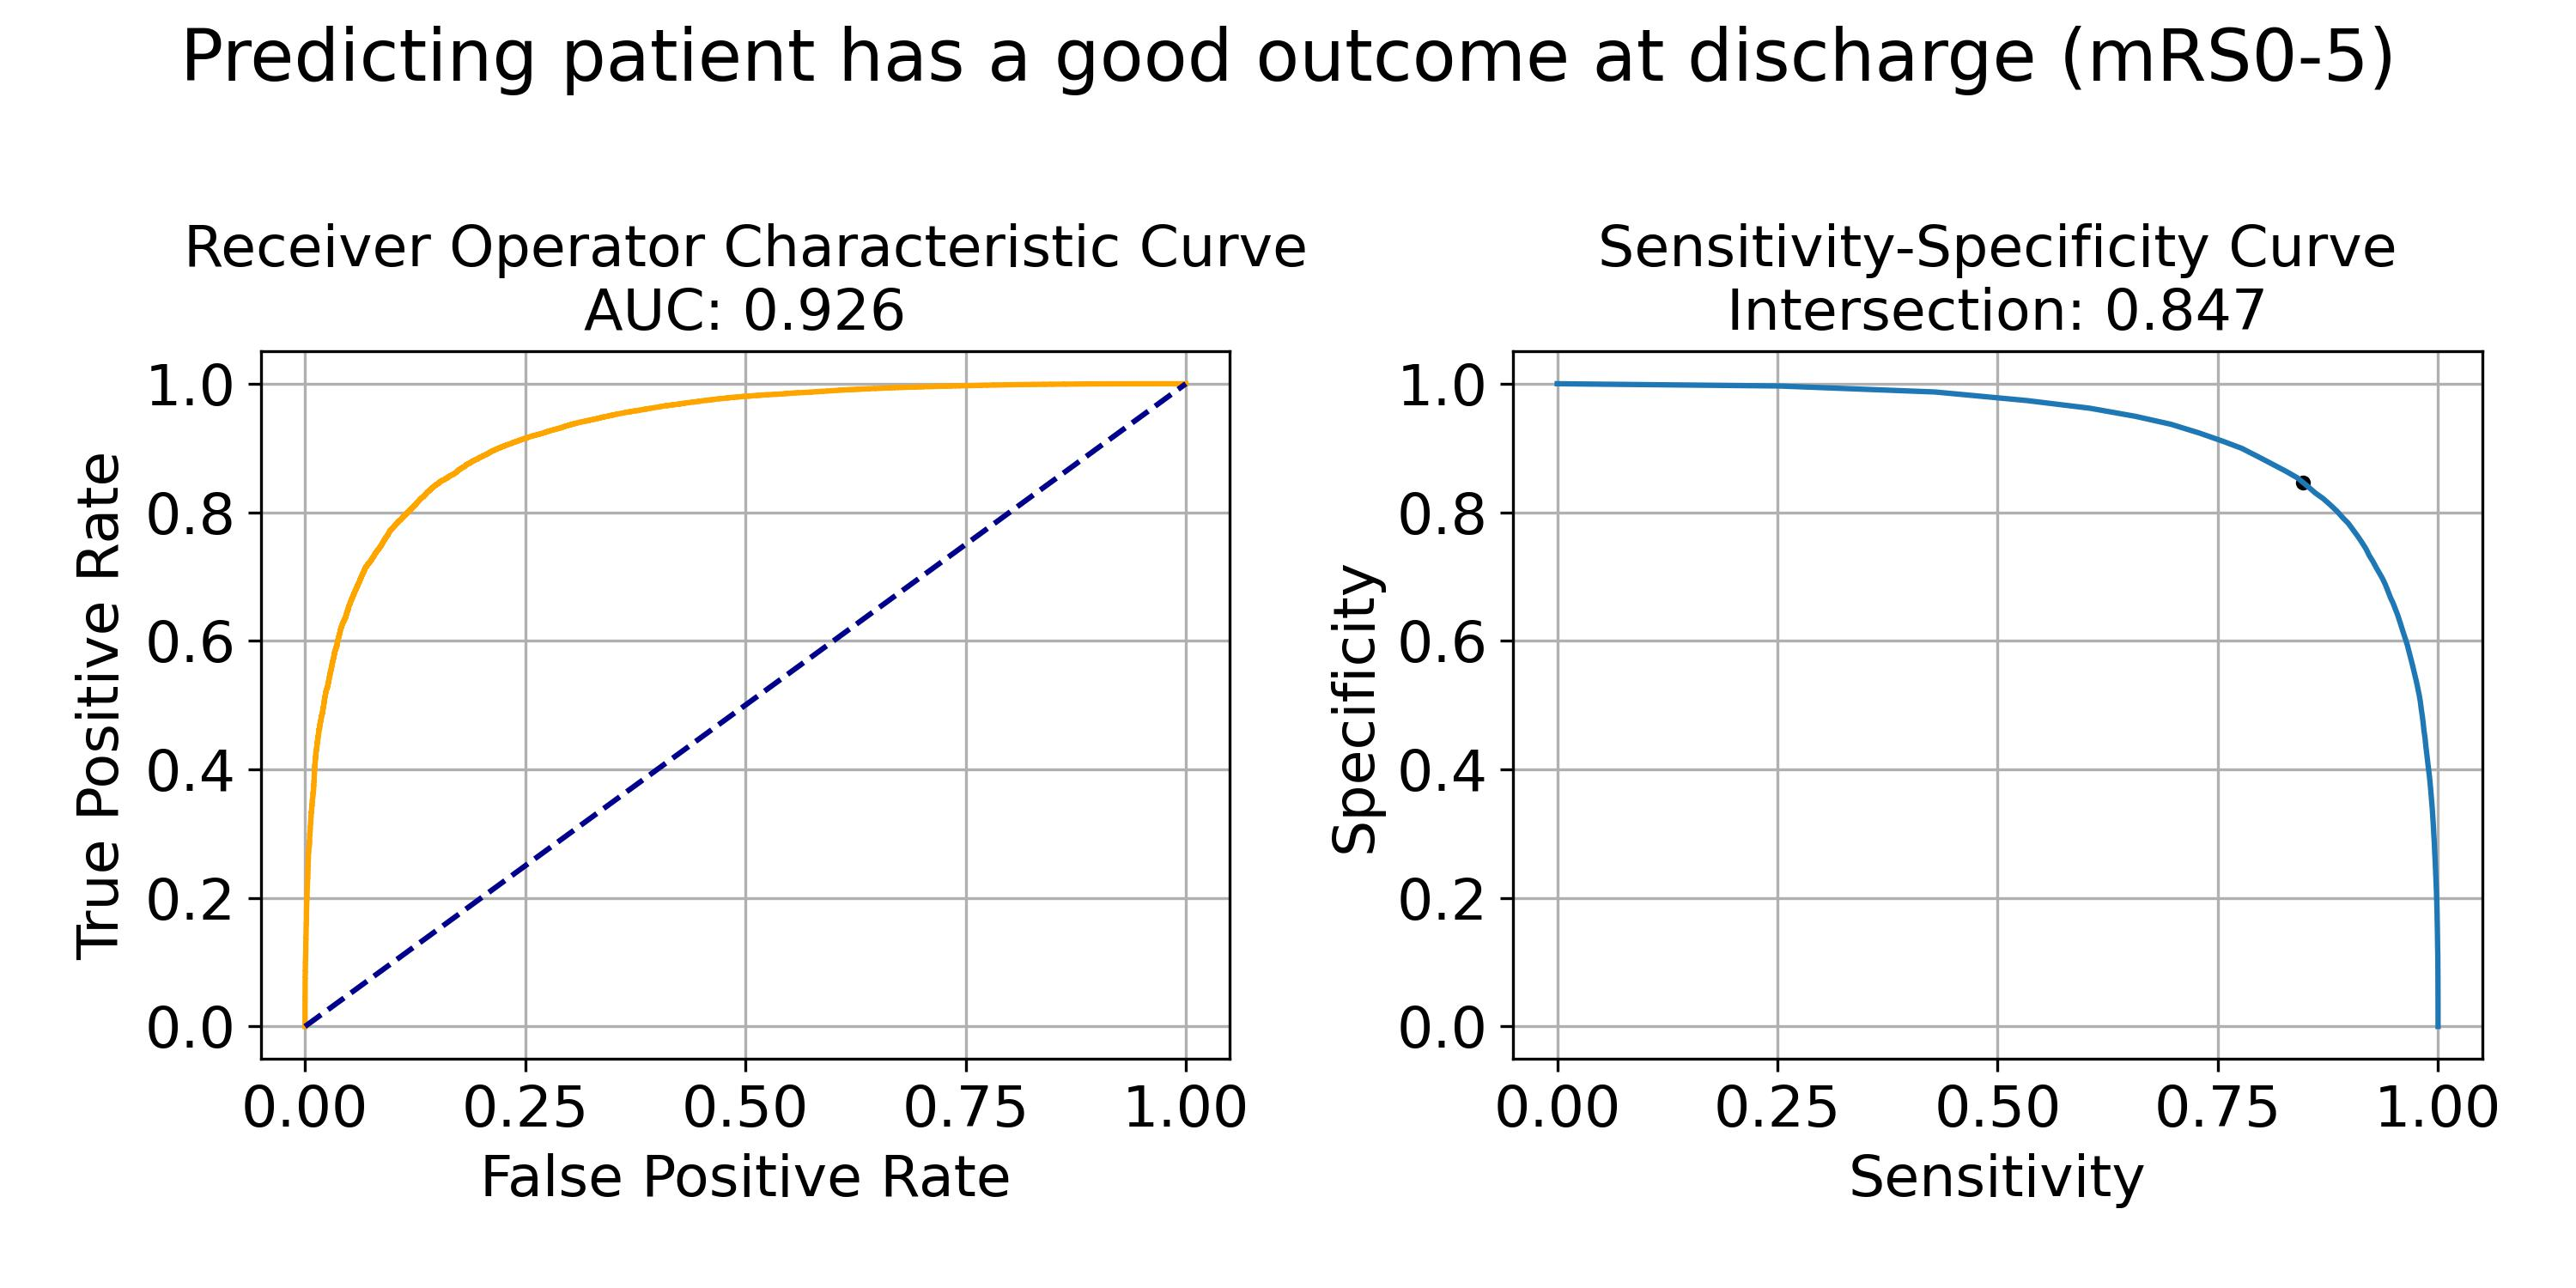
\includegraphics[width=0.5\linewidth]{./images/073_xgb_all_features_5fold_binary_roc_sens_spec_mrs5_kfold0_paper}}
    \label{fig:rocauc_ss_all_features}
  \caption{ROC AUC, and specificity and sensitivity plots for each of the mRS threshold levels to define a good outcome (for first kfold). All features as model inputs.}

\end{figure}






\subsection{Model accuracy}


Figure \ref{fig:feature_selection} shows the mean ROCAUC for the 5 kfold model, sequentially selecting the features.

\begin{figure}[!h]
    \centering
    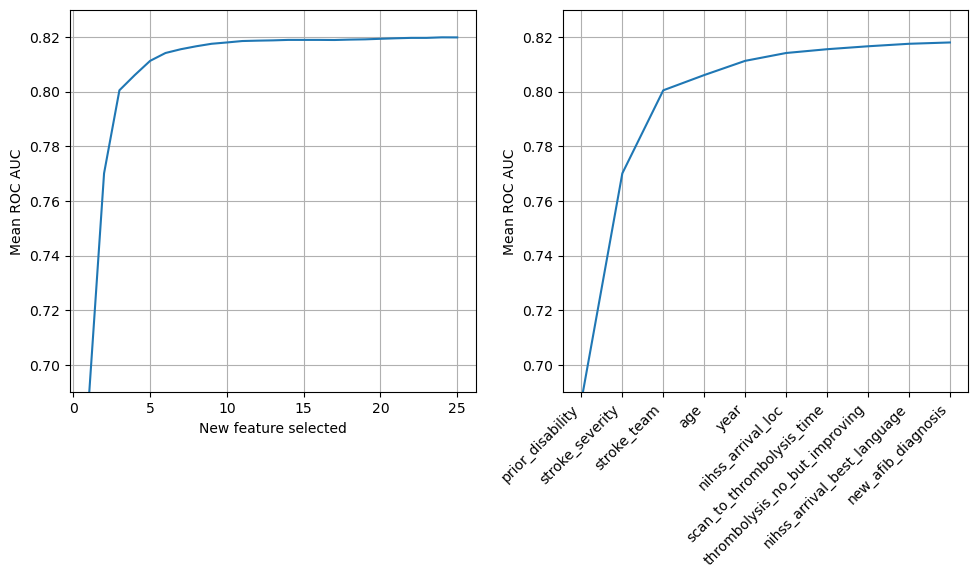
\includegraphics[width=0.75\textwidth]{./images/020_feature_selection.jpg}\\
    \caption{Feature selection}
    \label{fig:feature_selection}
\end{figure}

{ROCAUC}

Figure \ref{fig:confusion_rocauc} shows the ROCAUC results for the individual one vs one classes. There is a better performance for classes to be distiguishable when they are further from each other in value. 

\begin{figure}
    \centering
    {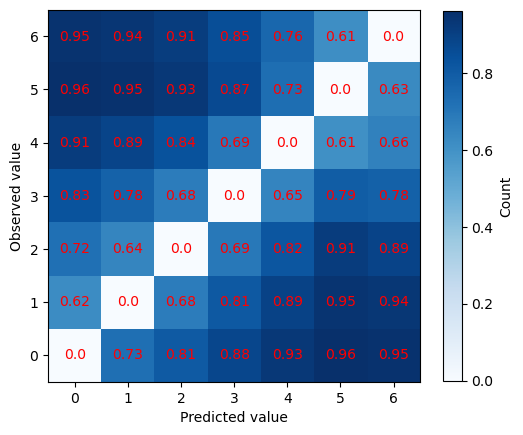
\includegraphics[width = 4in]{./images/040_ROCAUC_confusion_matrix_ovo.png}}\\
    \caption{}
    \label{fig:confusion_rocauc}
\end{figure}

Figure \ref{fig:confusion_mrs} shows the confusion matrices for the 5 kfolds. Given the consistency across the 5 kfolds, we will now only use results from the first kfold.

\begin{figure}[!h]
    \centering
    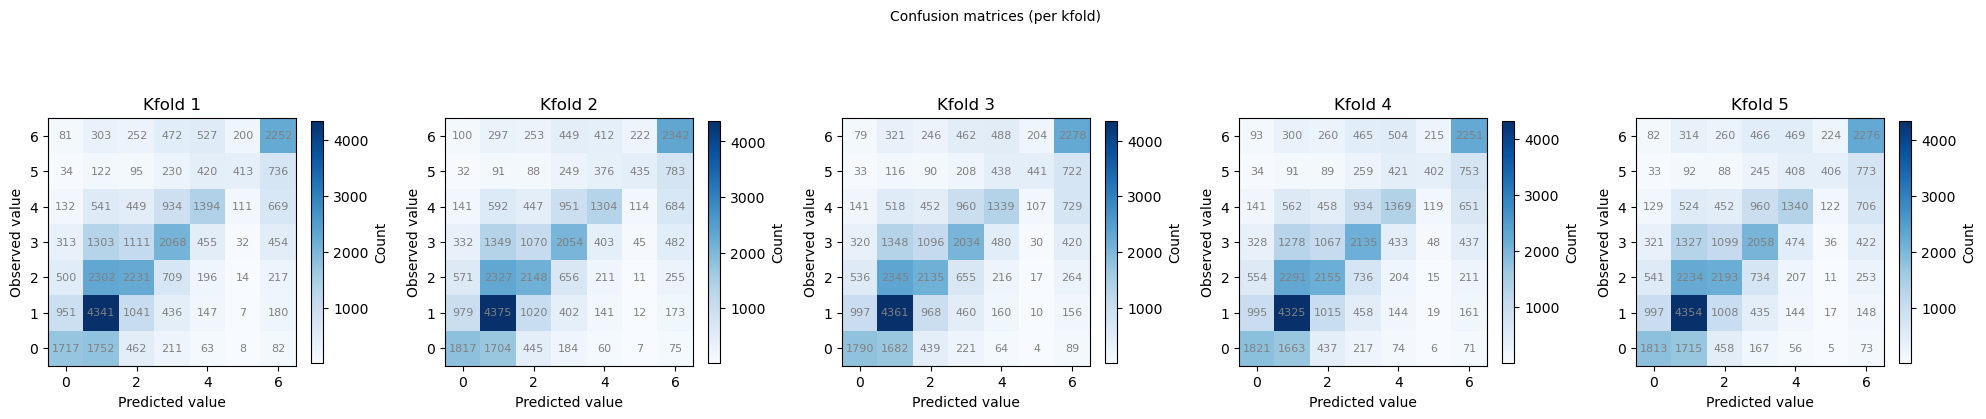
\includegraphics[trim={0 0 0 1.2cm}, clip, width=1\textwidth]{./images/040_confusion_matrices_5fold.png}\\
    \caption{}
    \label{fig:confusion_mrs}
\end{figure}


\section{Method}

\subsection{Data}

Data were retrieved for 168,347 emergency stroke admissions to acute stroke teams in England for six years, 2016–2021 (inclusive), obtained from the Sentinel Stroke National Audit Programme (SSNAP). Data fields were provided for the hyper-acute phase of the stroke pathway, up to and including our target feature: disability on inpatient discharge. Disability is recorded in the SSNAP dataset using the modified Rankin Scale (mRS), where mRS 0 represents perfect health and mRS 6 represents death. The data includes 118 acute stroke hospitals (each has at least 250 stroke admissions and delivers thrombolysis to at least 10 patients in the six years).

\subsection{Machine learning models}

\subsection{Model accuracy}

\begin{figure}[!h]
    \centering
    \begin{subfigure}[b]{1\textwidth}
      \centering
      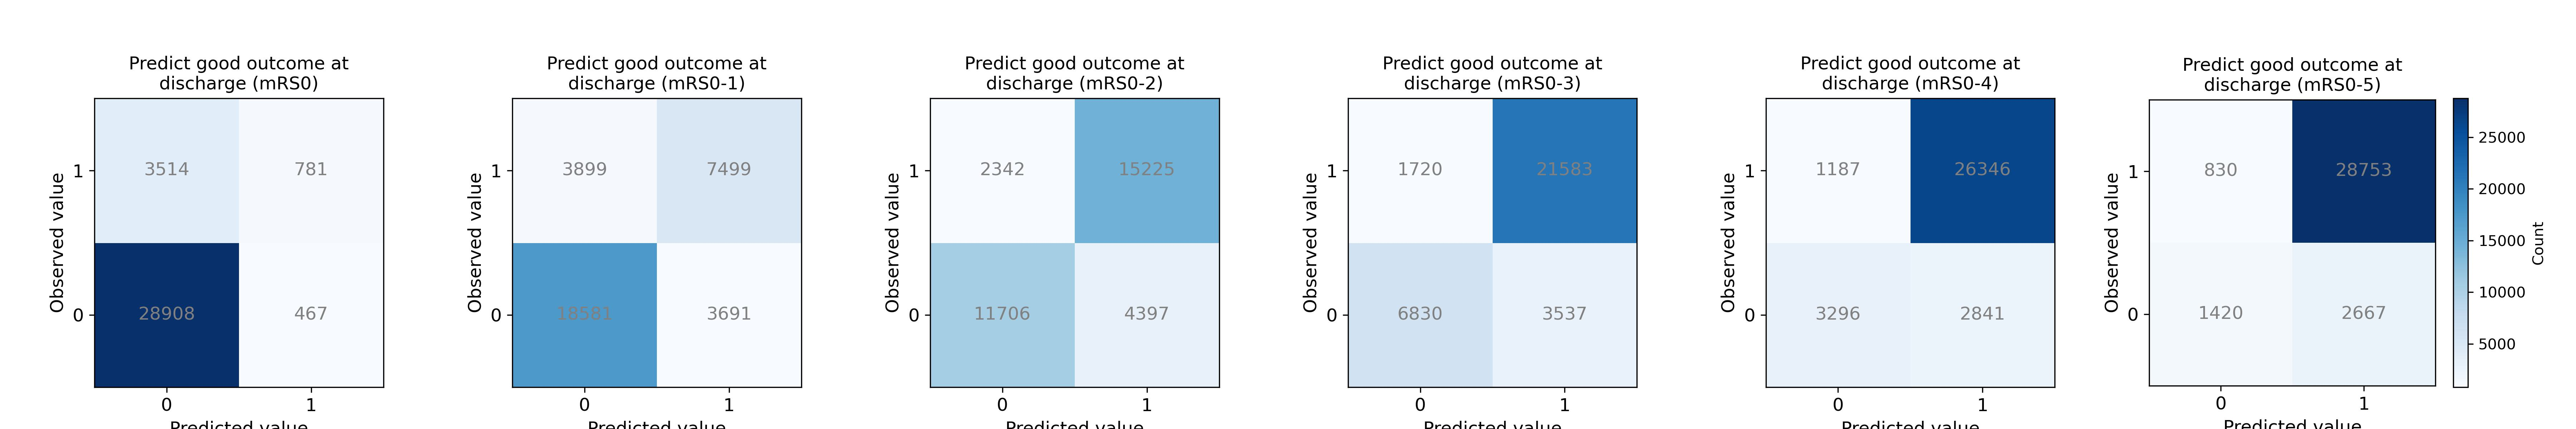
\includegraphics[width=1\textwidth]{./images/083_xgb_7_features_5fold_binary_confusion_matrices_per_binary_threshold_kfold0}\\
      \caption{Kfold 1}
      \label{fig:results_waterfall}
    \end{subfigure}
    \hfill
    \begin{subfigure}[b]{1\textwidth}
      \centering    
      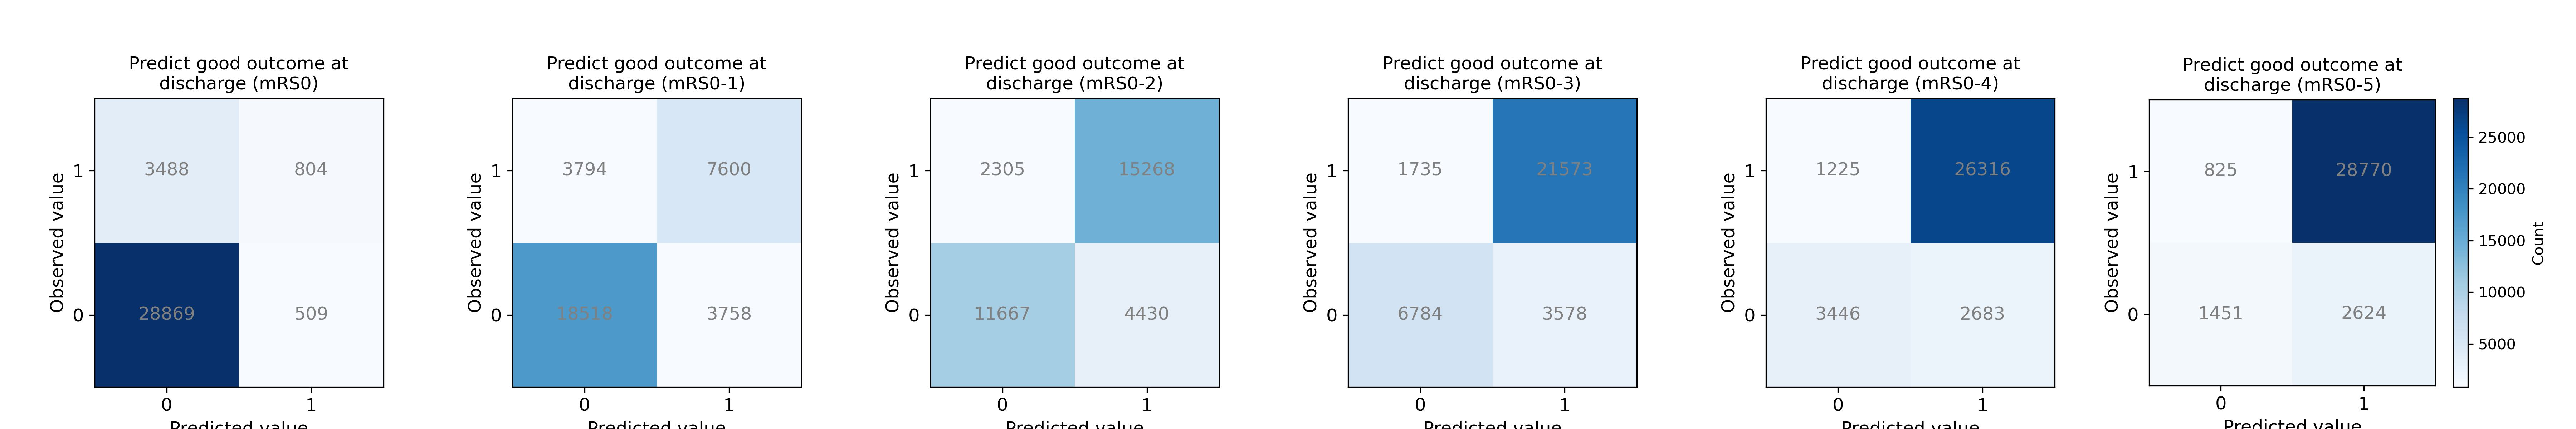
\includegraphics[width=1\textwidth]{./images/083_xgb_7_features_5fold_binary_confusion_matrices_per_binary_threshold_kfold1}\\
      \caption{Kfold 2}
      \label{fig:results_waterfall}
    \end{subfigure}
    \hfill
    \begin{subfigure}[b]{1\textwidth}
      \centering
      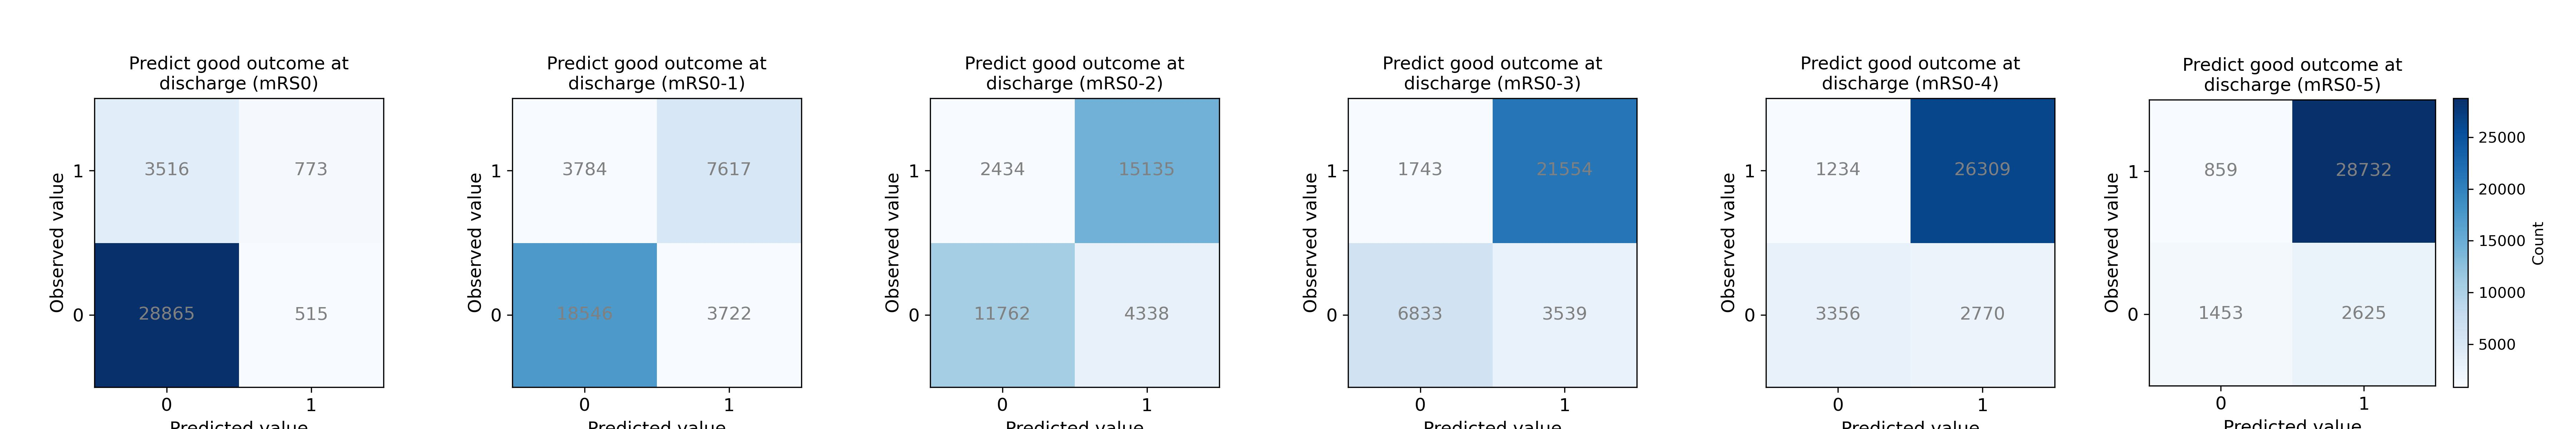
\includegraphics[width=1\textwidth]{./images/083_xgb_7_features_5fold_binary_confusion_matrices_per_binary_threshold_kfold2}\\
      \caption{Kfold 3}
      \label{fig:results_waterfall}
    \end{subfigure}
    \hfill
    \begin{subfigure}[b]{1\textwidth}
      \centering
      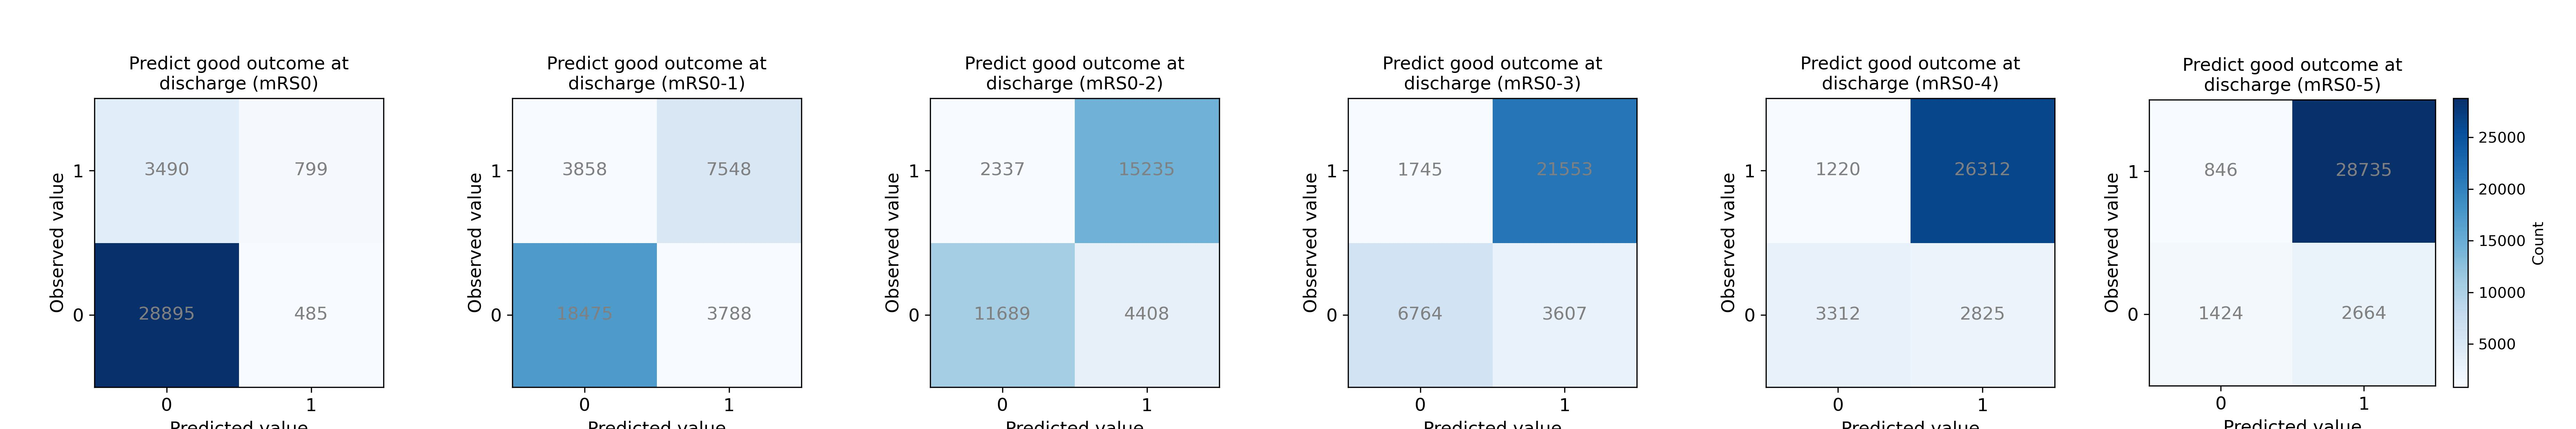
\includegraphics[width=1\textwidth]{./images/083_xgb_7_features_5fold_binary_confusion_matrices_per_binary_threshold_kfold3}\\
      \caption{Kfold 4}
      \label{fig:results_waterfall}
    \end{subfigure}
    \hfill
    \begin{subfigure}[b]{1\textwidth}
      \centering
      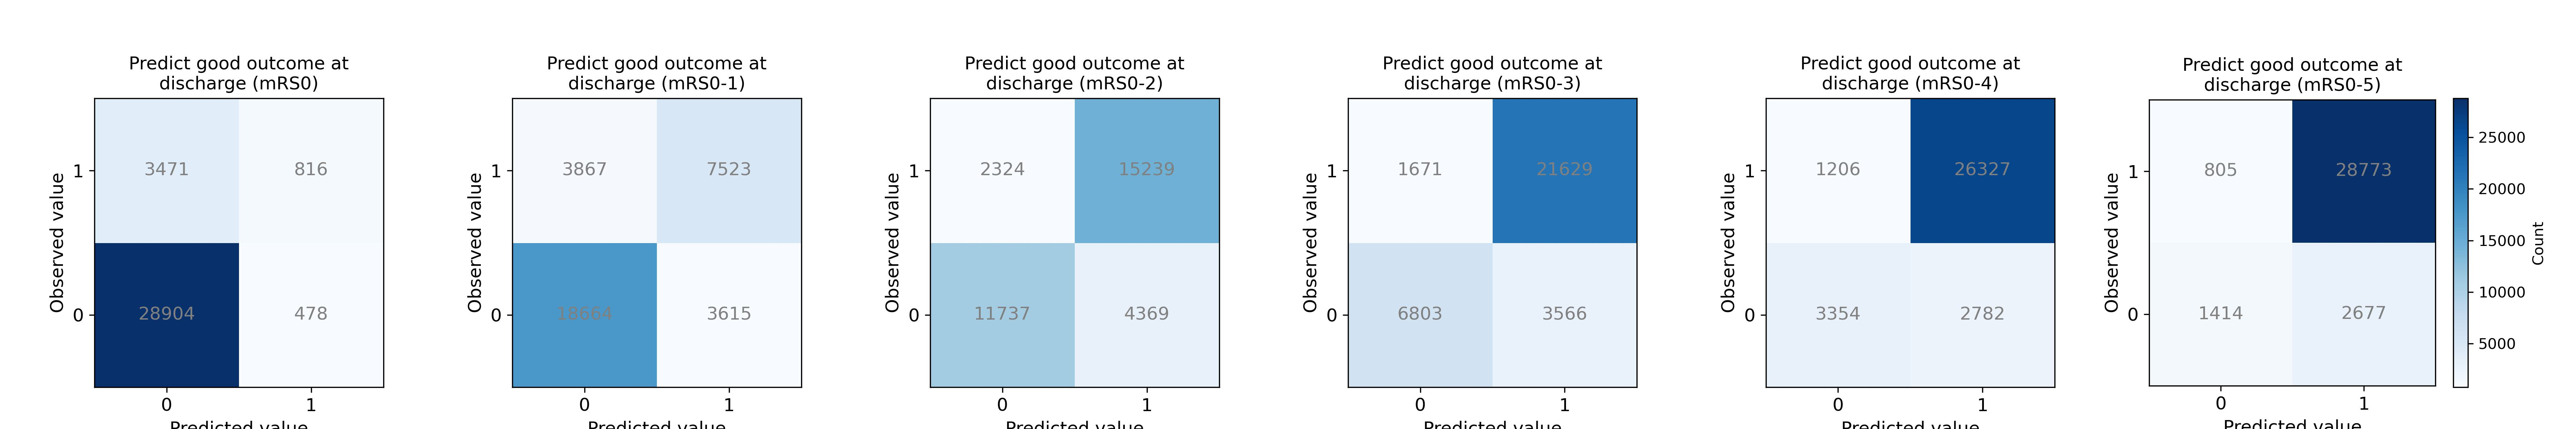
\includegraphics[width=1\textwidth]{./images/083_xgb_7_features_5fold_binary_confusion_matrices_per_binary_threshold_kfold4}\\
      \caption{Kfold 5}
      \label{fig:results_waterfall}
    \end{subfigure}
  \caption{Confusion matrices for each kfold (model with 7 features)}
\end{figure}


\begin{figure}[!ht]
\centering
    \subfloat[]{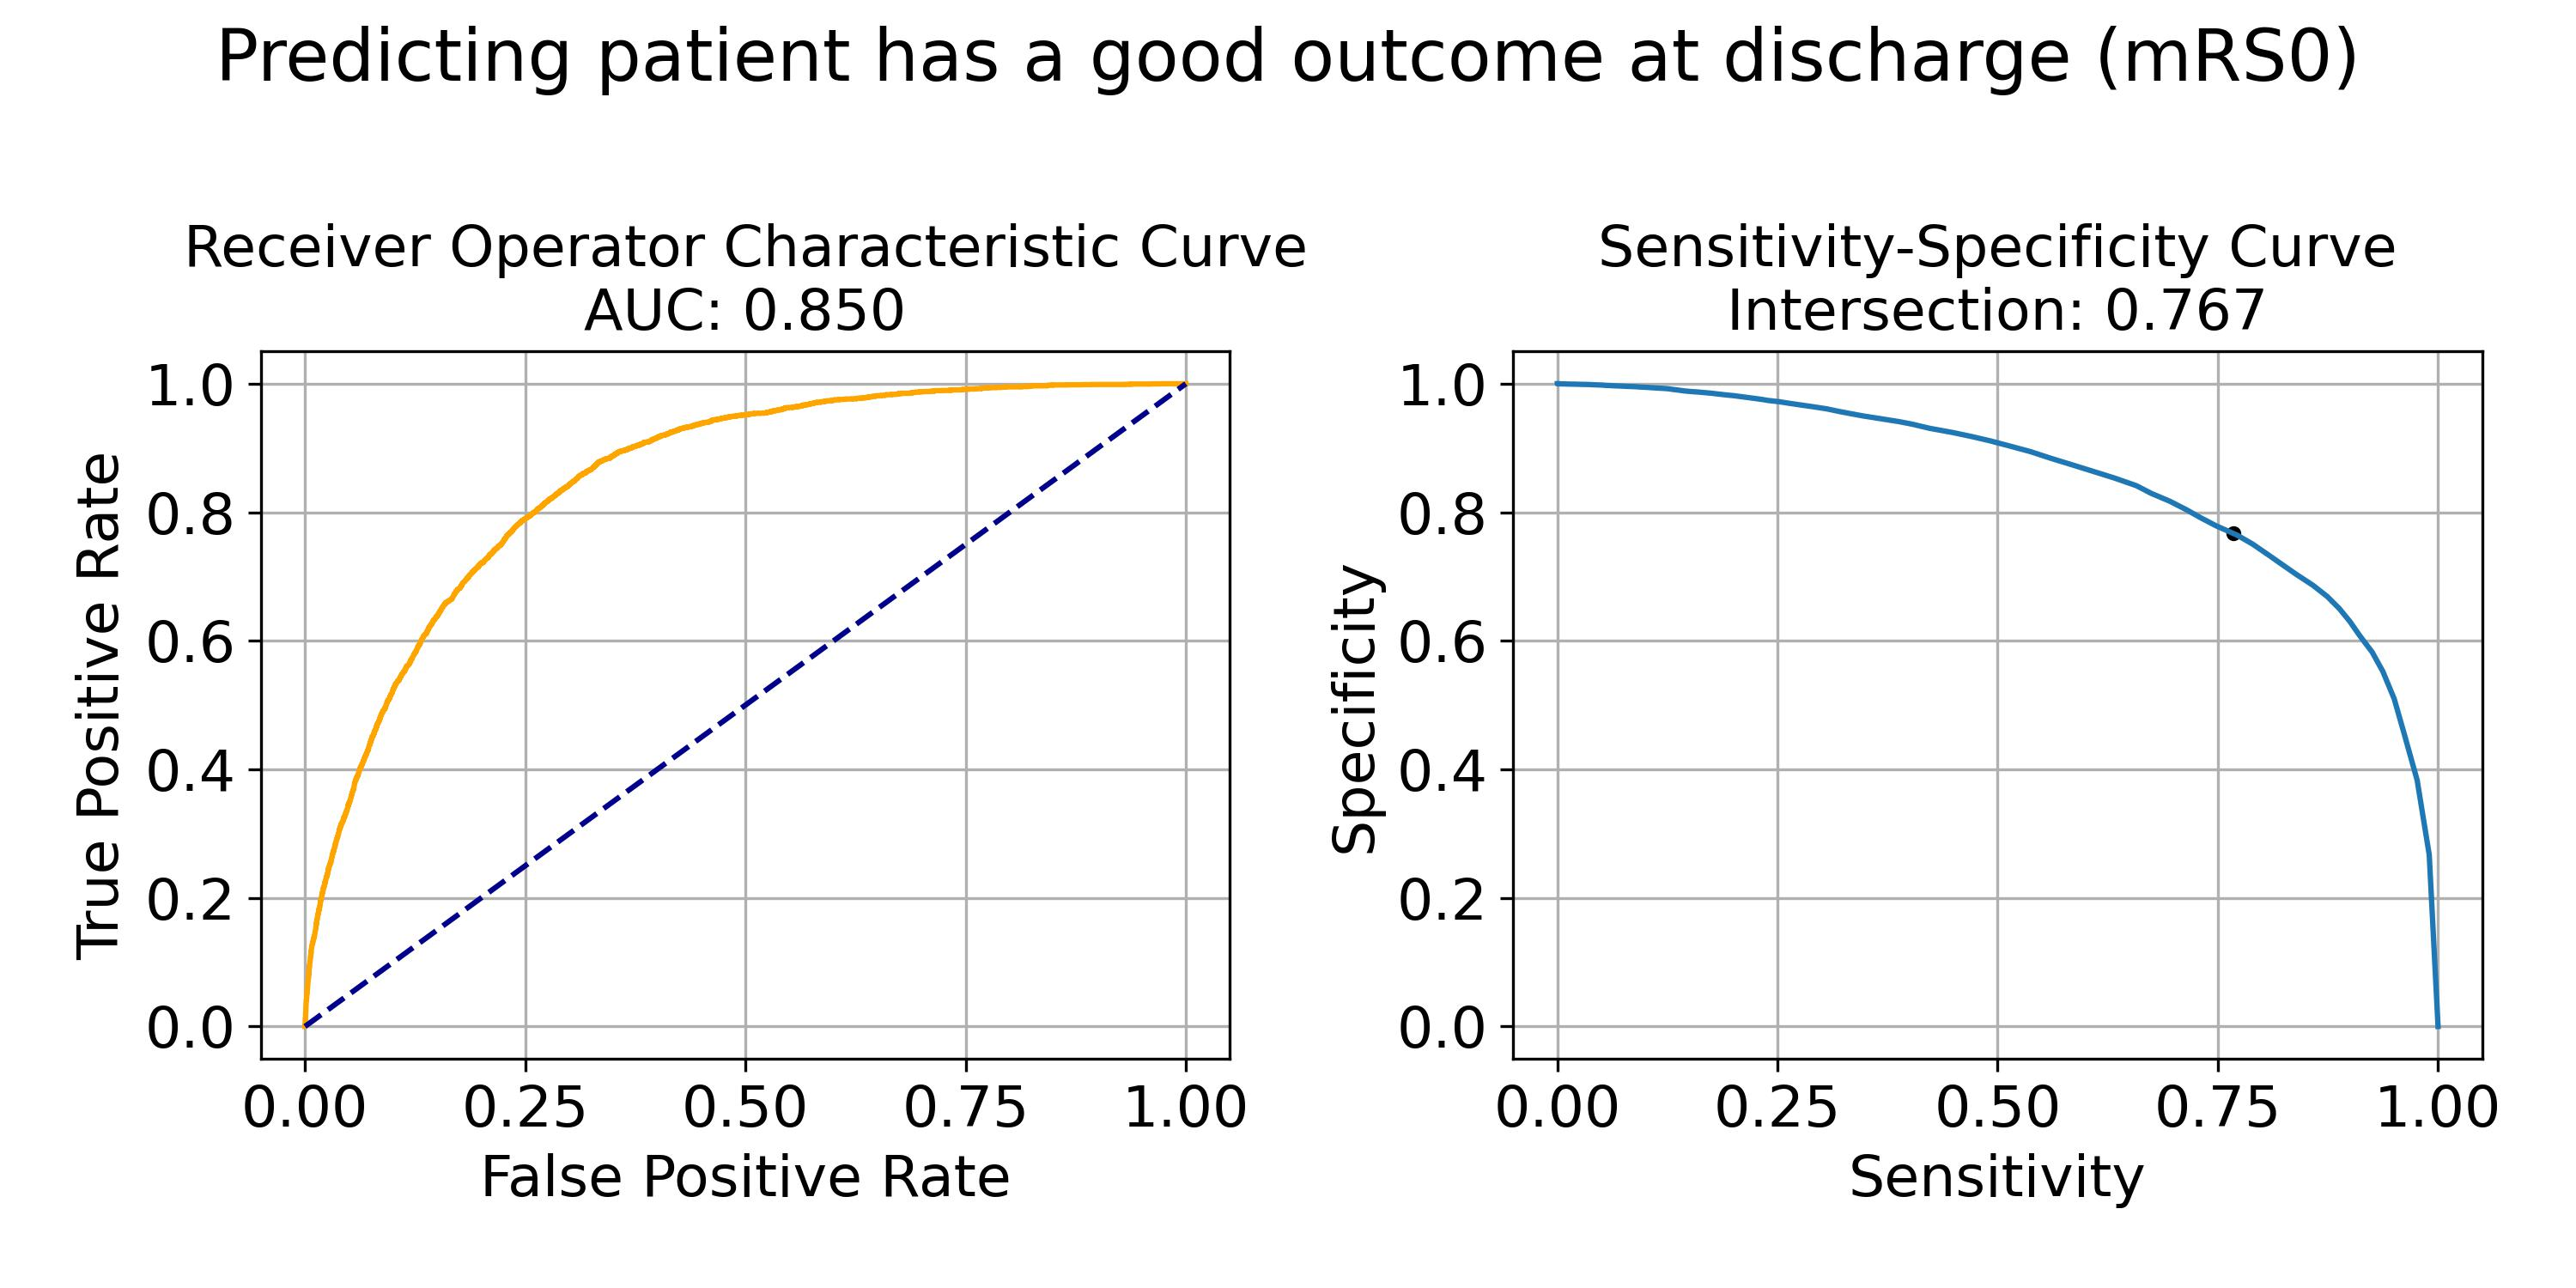
\includegraphics[width=0.5\linewidth]{./images/083_xgb_7_features_5fold_binary_roc_sens_spec_mrs0_kfold0_paper}}
\hfil
    \subfloat[]{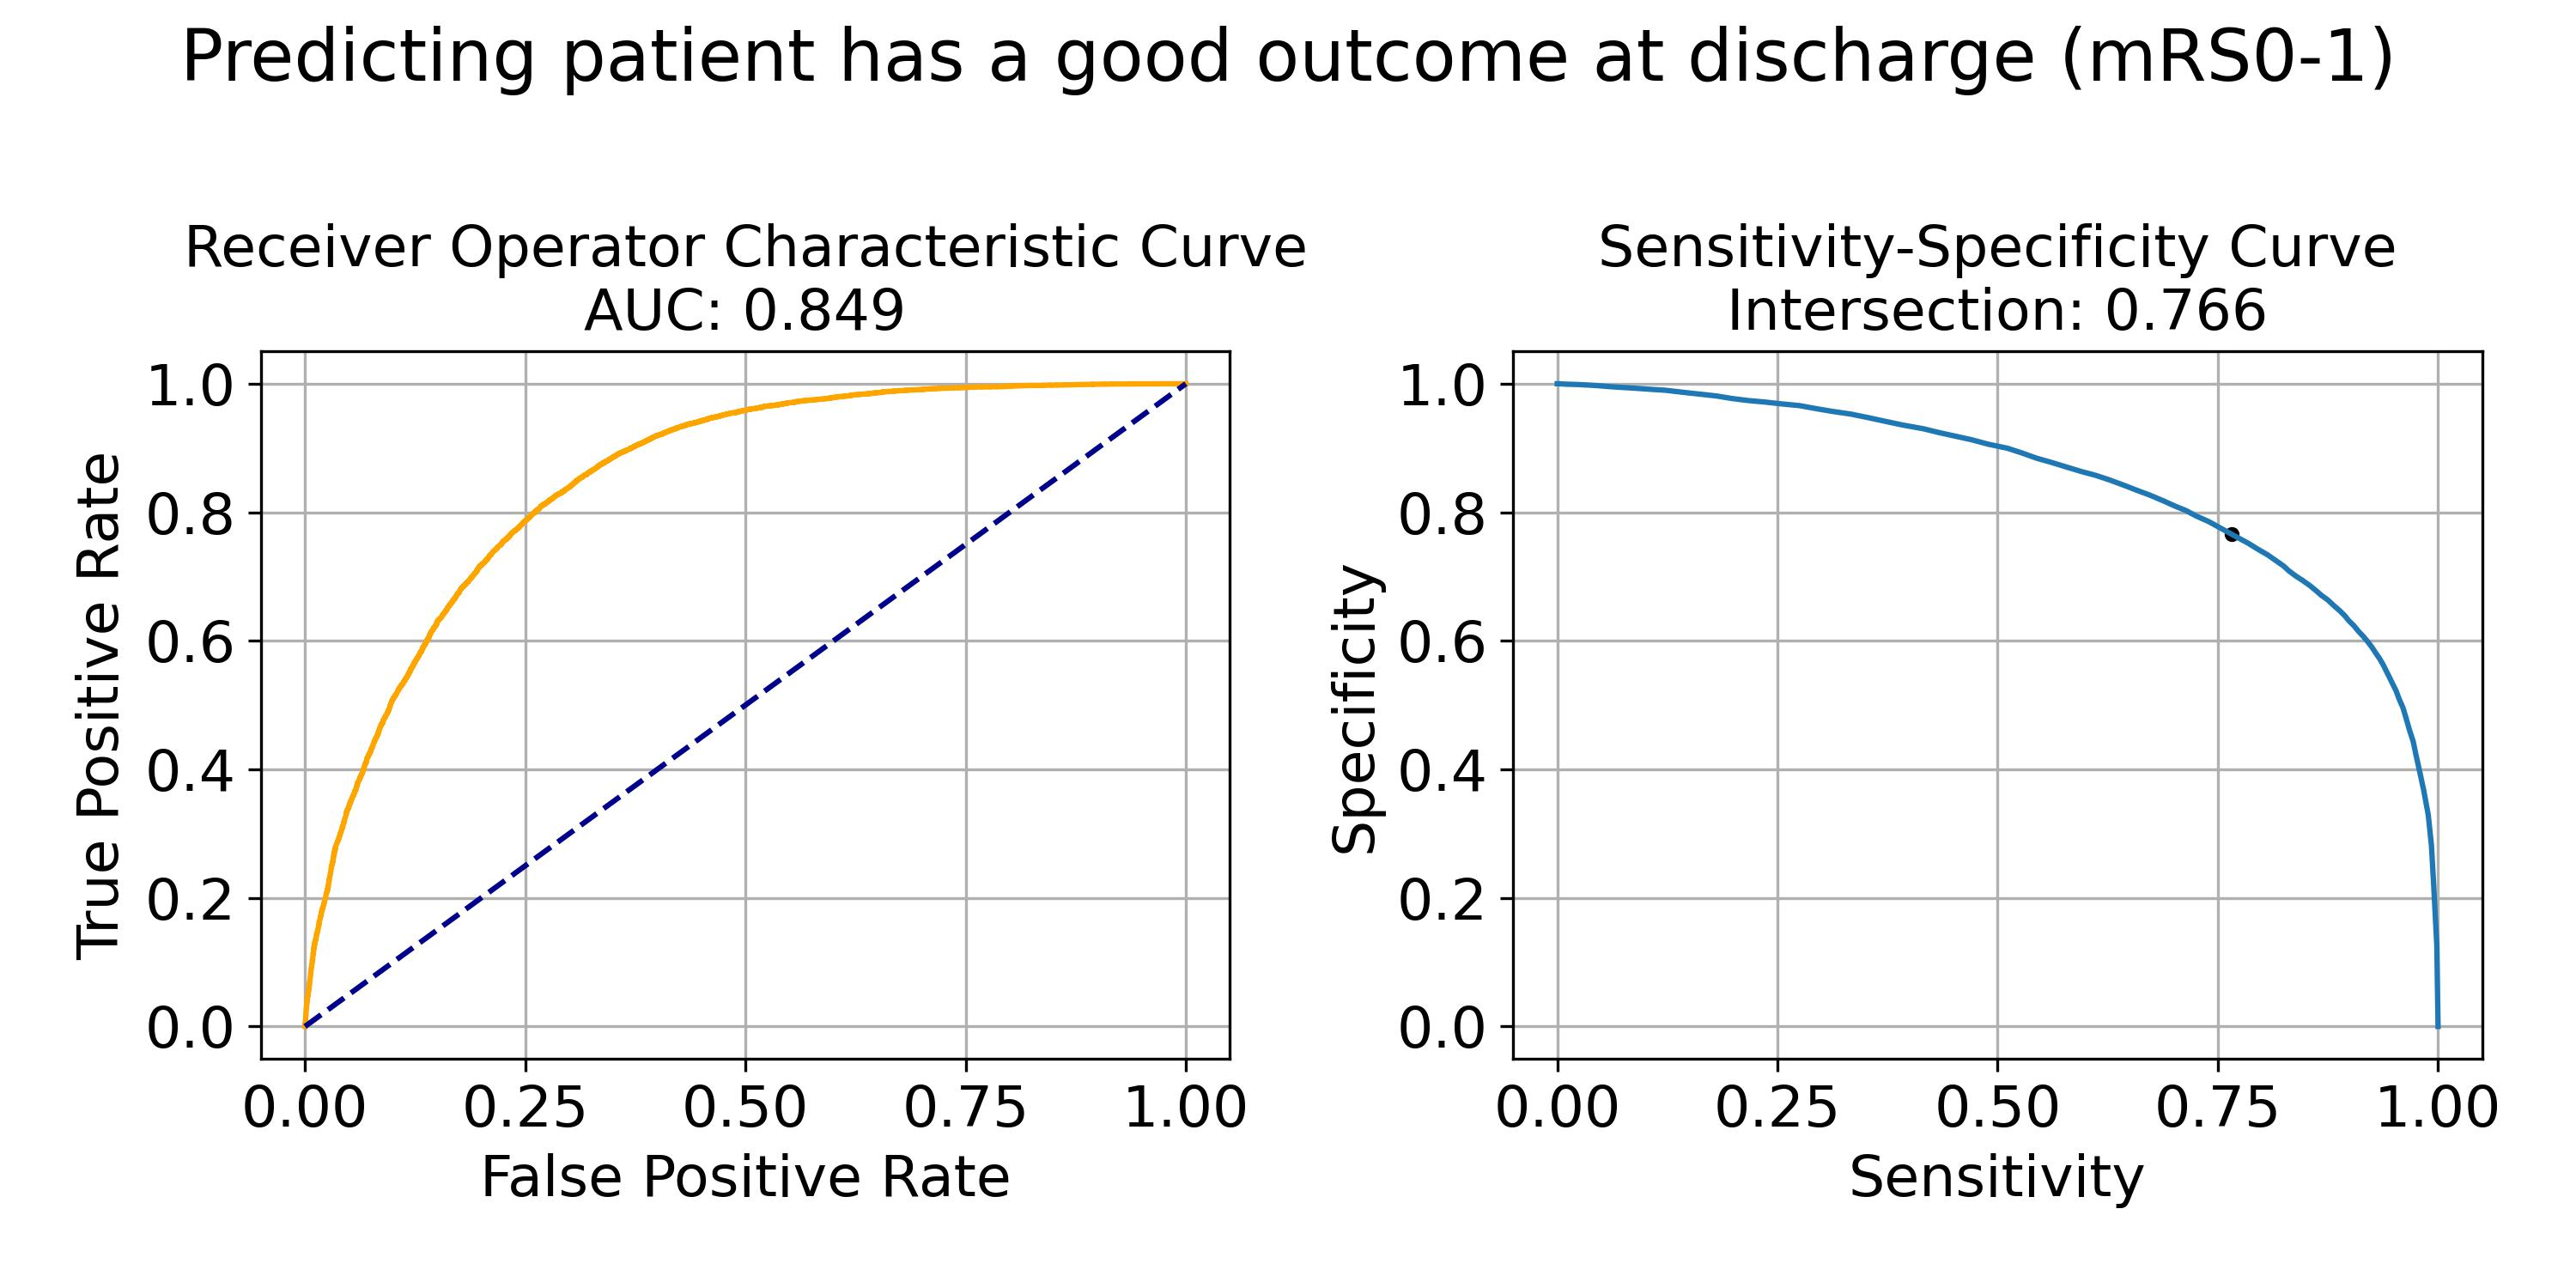
\includegraphics[width=0.5\linewidth]{./images/083_xgb_7_features_5fold_binary_roc_sens_spec_mrs1_kfold0_paper}}

    \subfloat[]{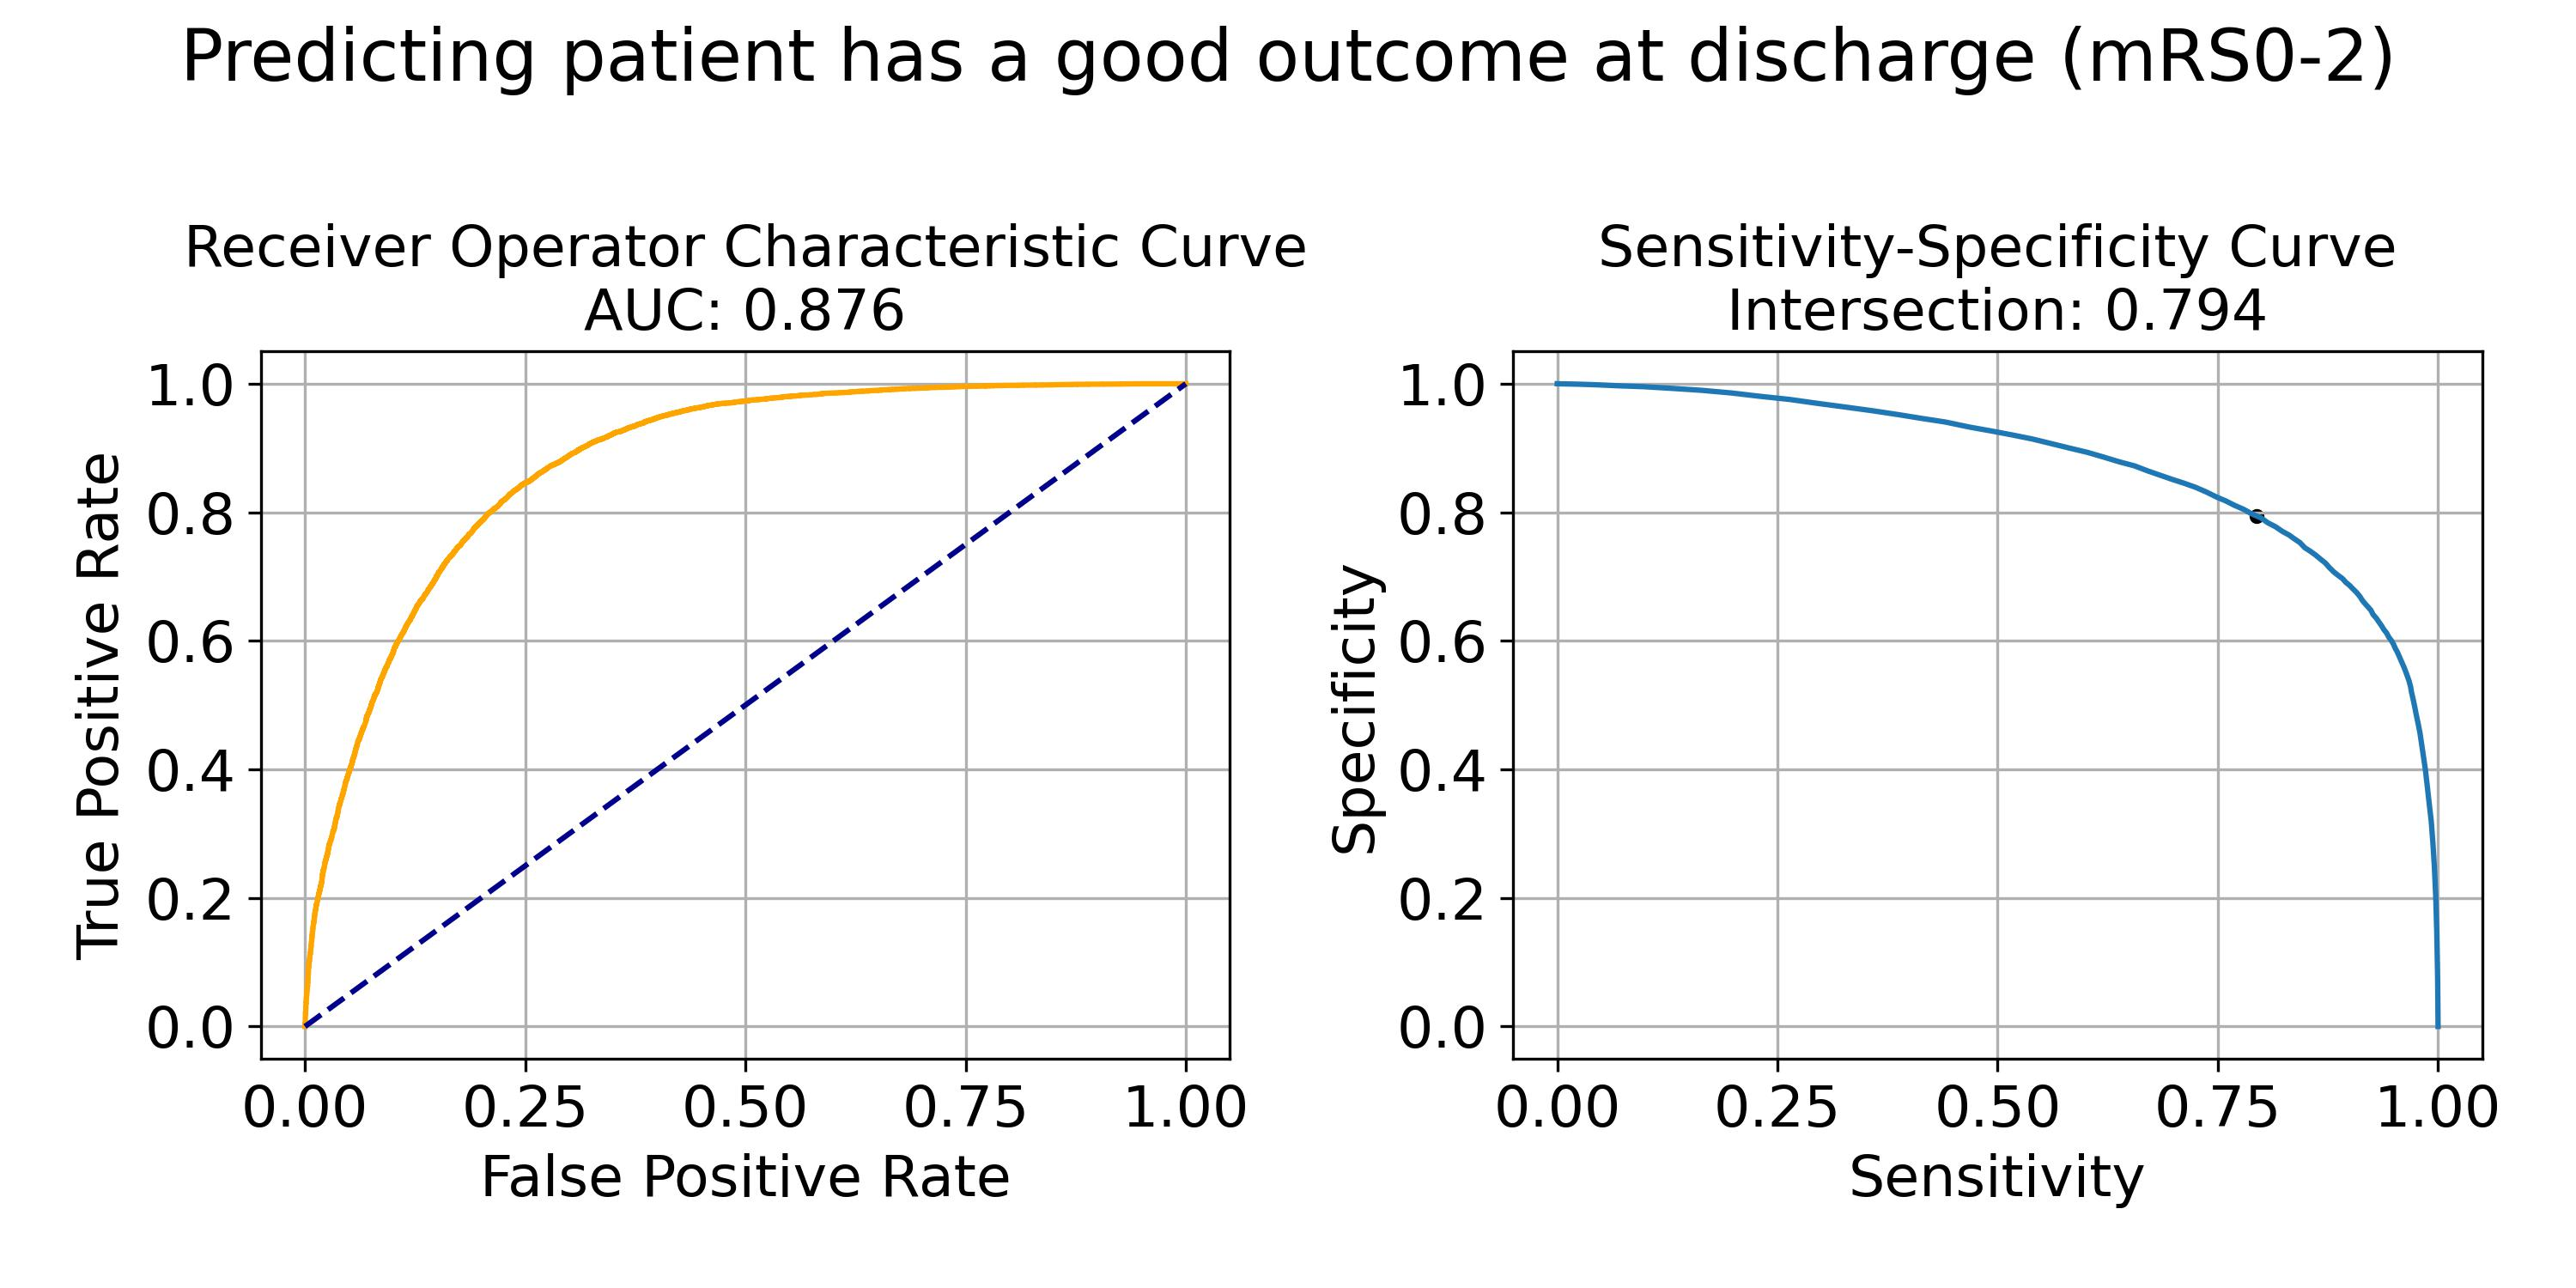
\includegraphics[width=0.5\linewidth]{./images/083_xgb_7_features_5fold_binary_roc_sens_spec_mrs2_kfold0_paper}}
\hfil
    \subfloat[]{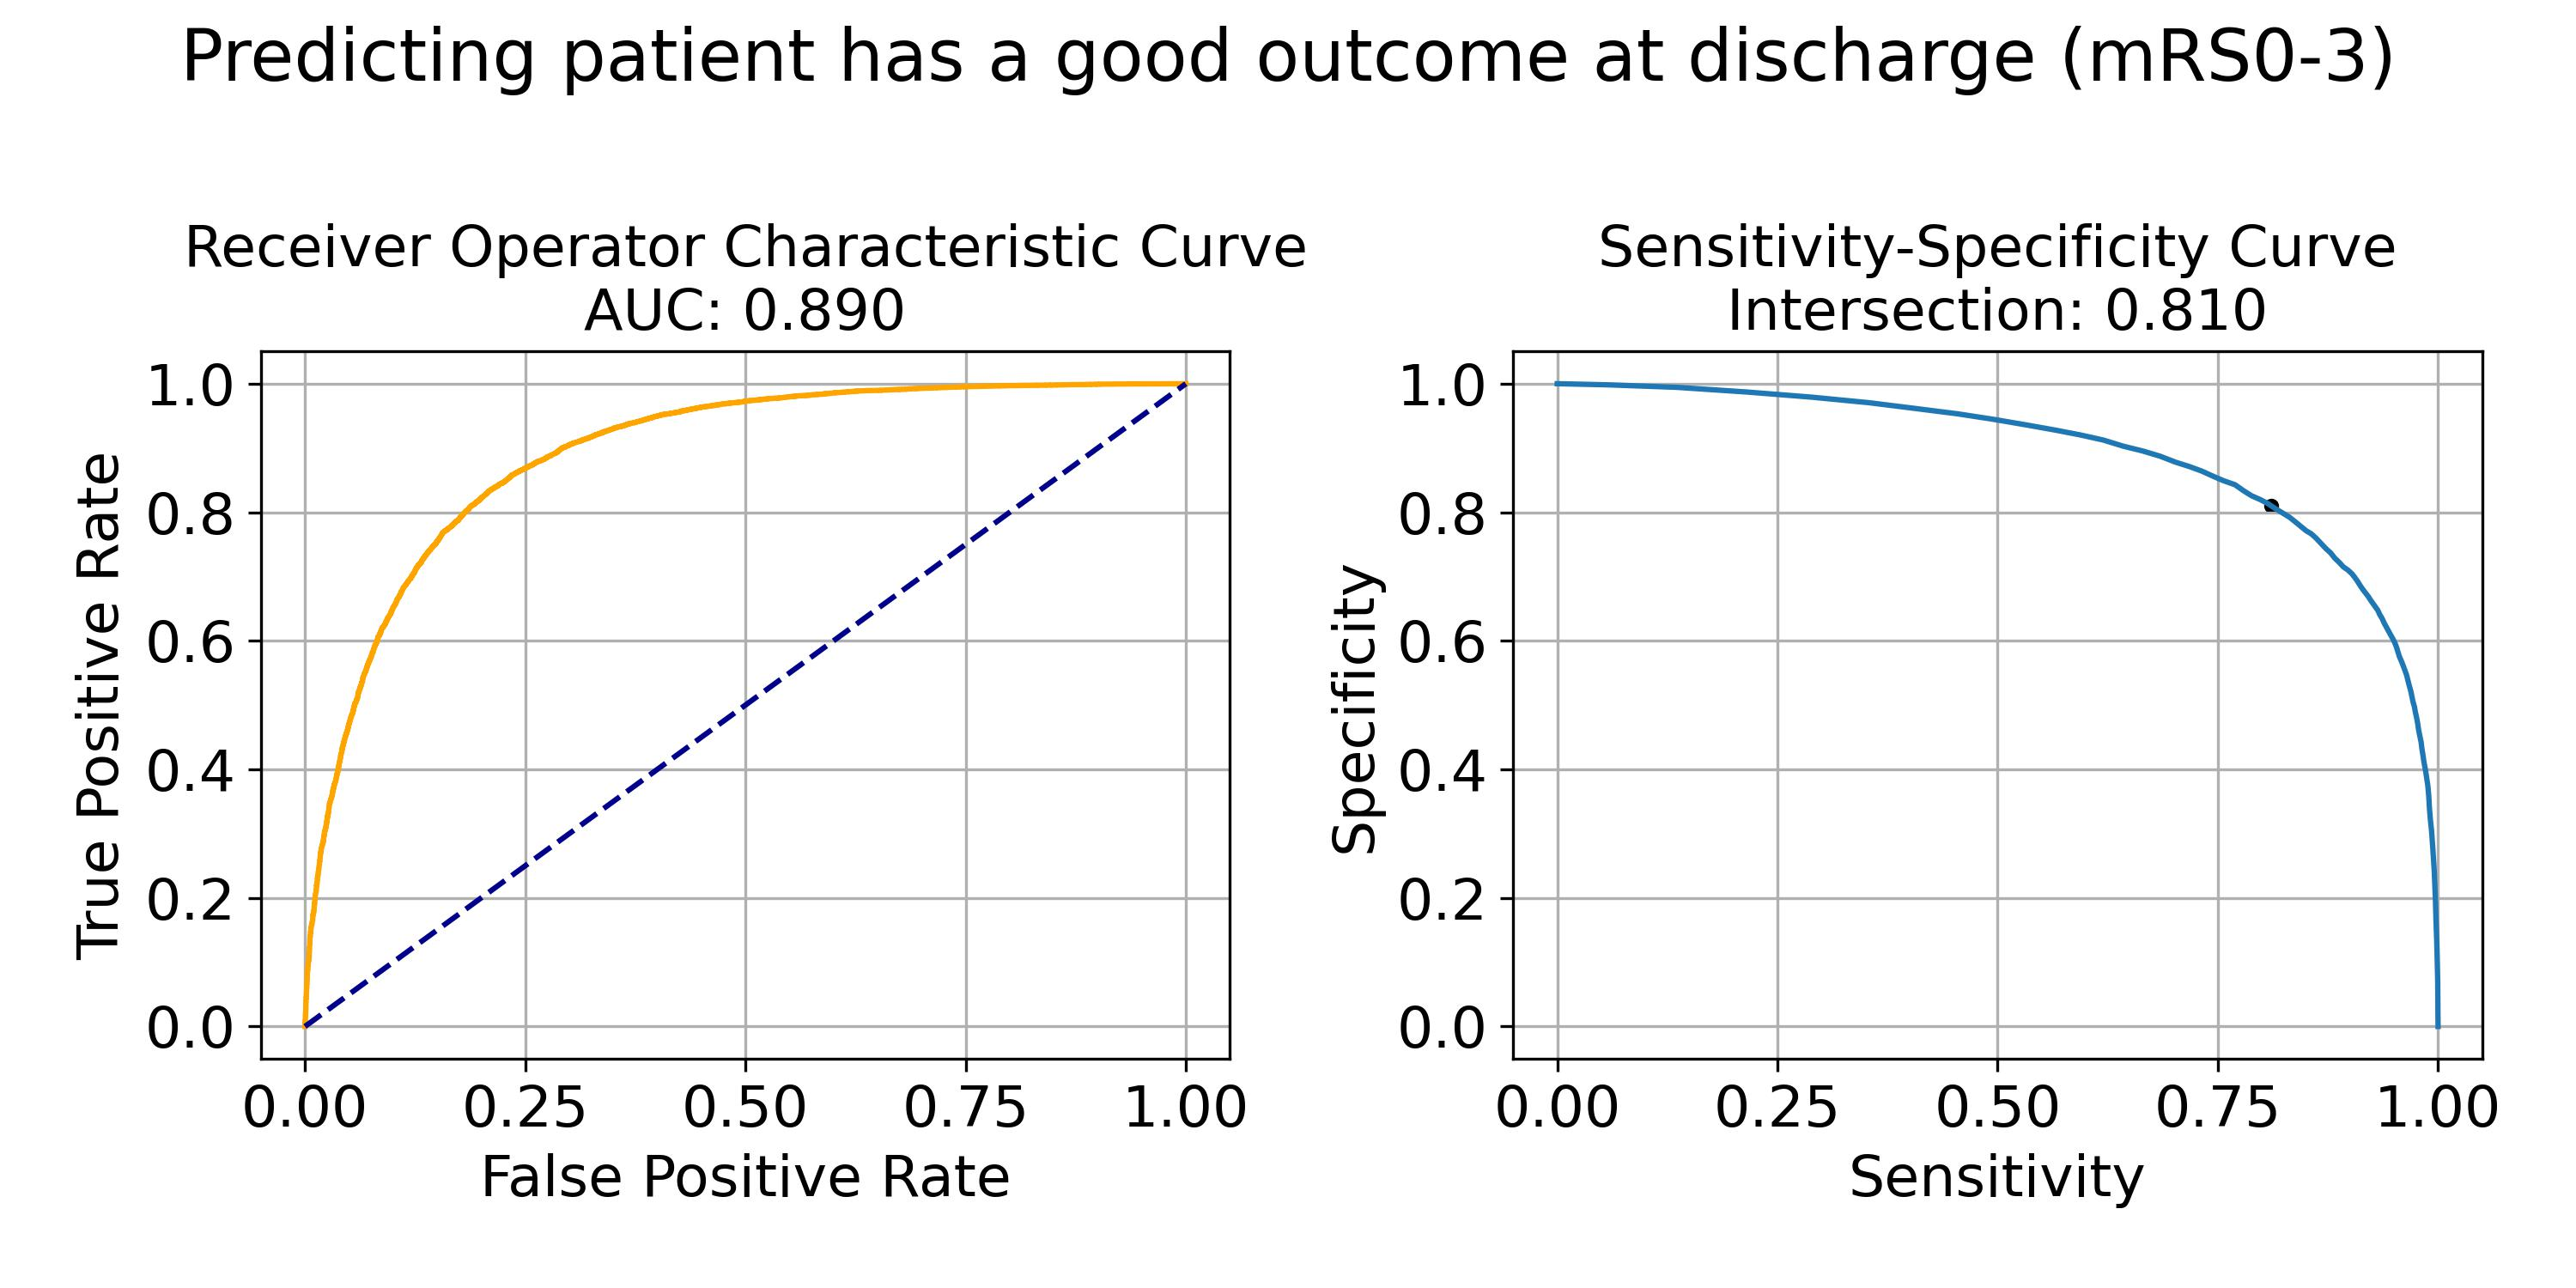
\includegraphics[width=0.5\linewidth]{./images/083_xgb_7_features_5fold_binary_roc_sens_spec_mrs3_kfold0_paper}}

    \subfloat[]{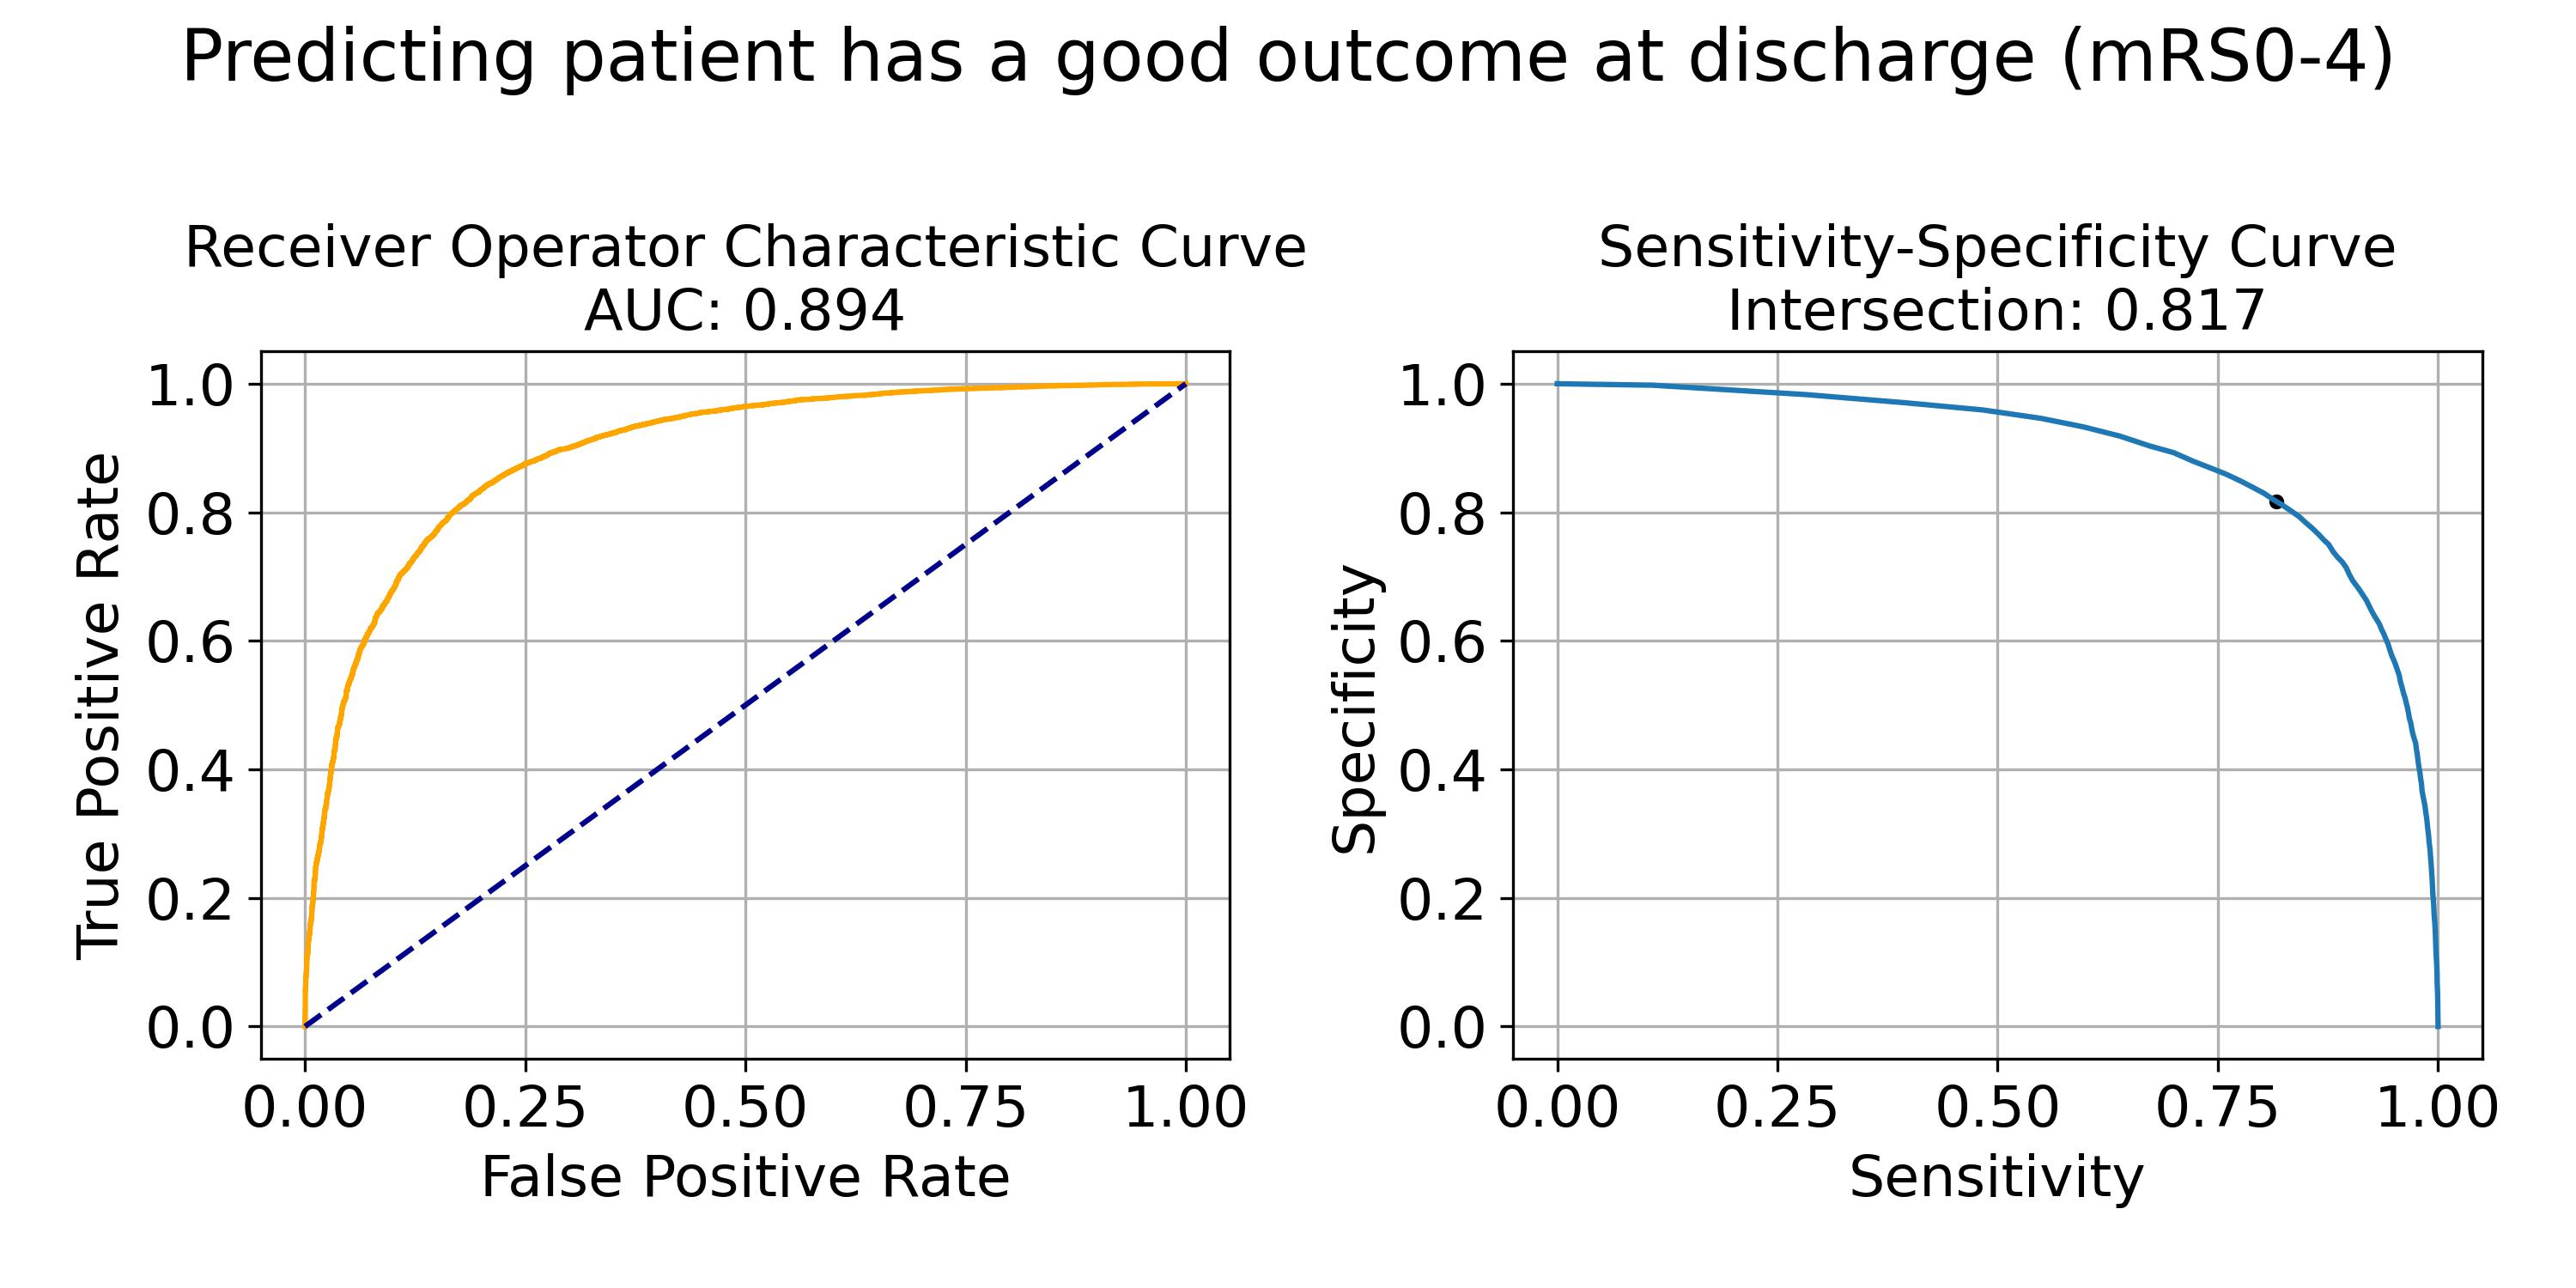
\includegraphics[width=0.5\linewidth]{./images/083_xgb_7_features_5fold_binary_roc_sens_spec_mrs4_kfold0_paper}}
\hfil
    \subfloat[]{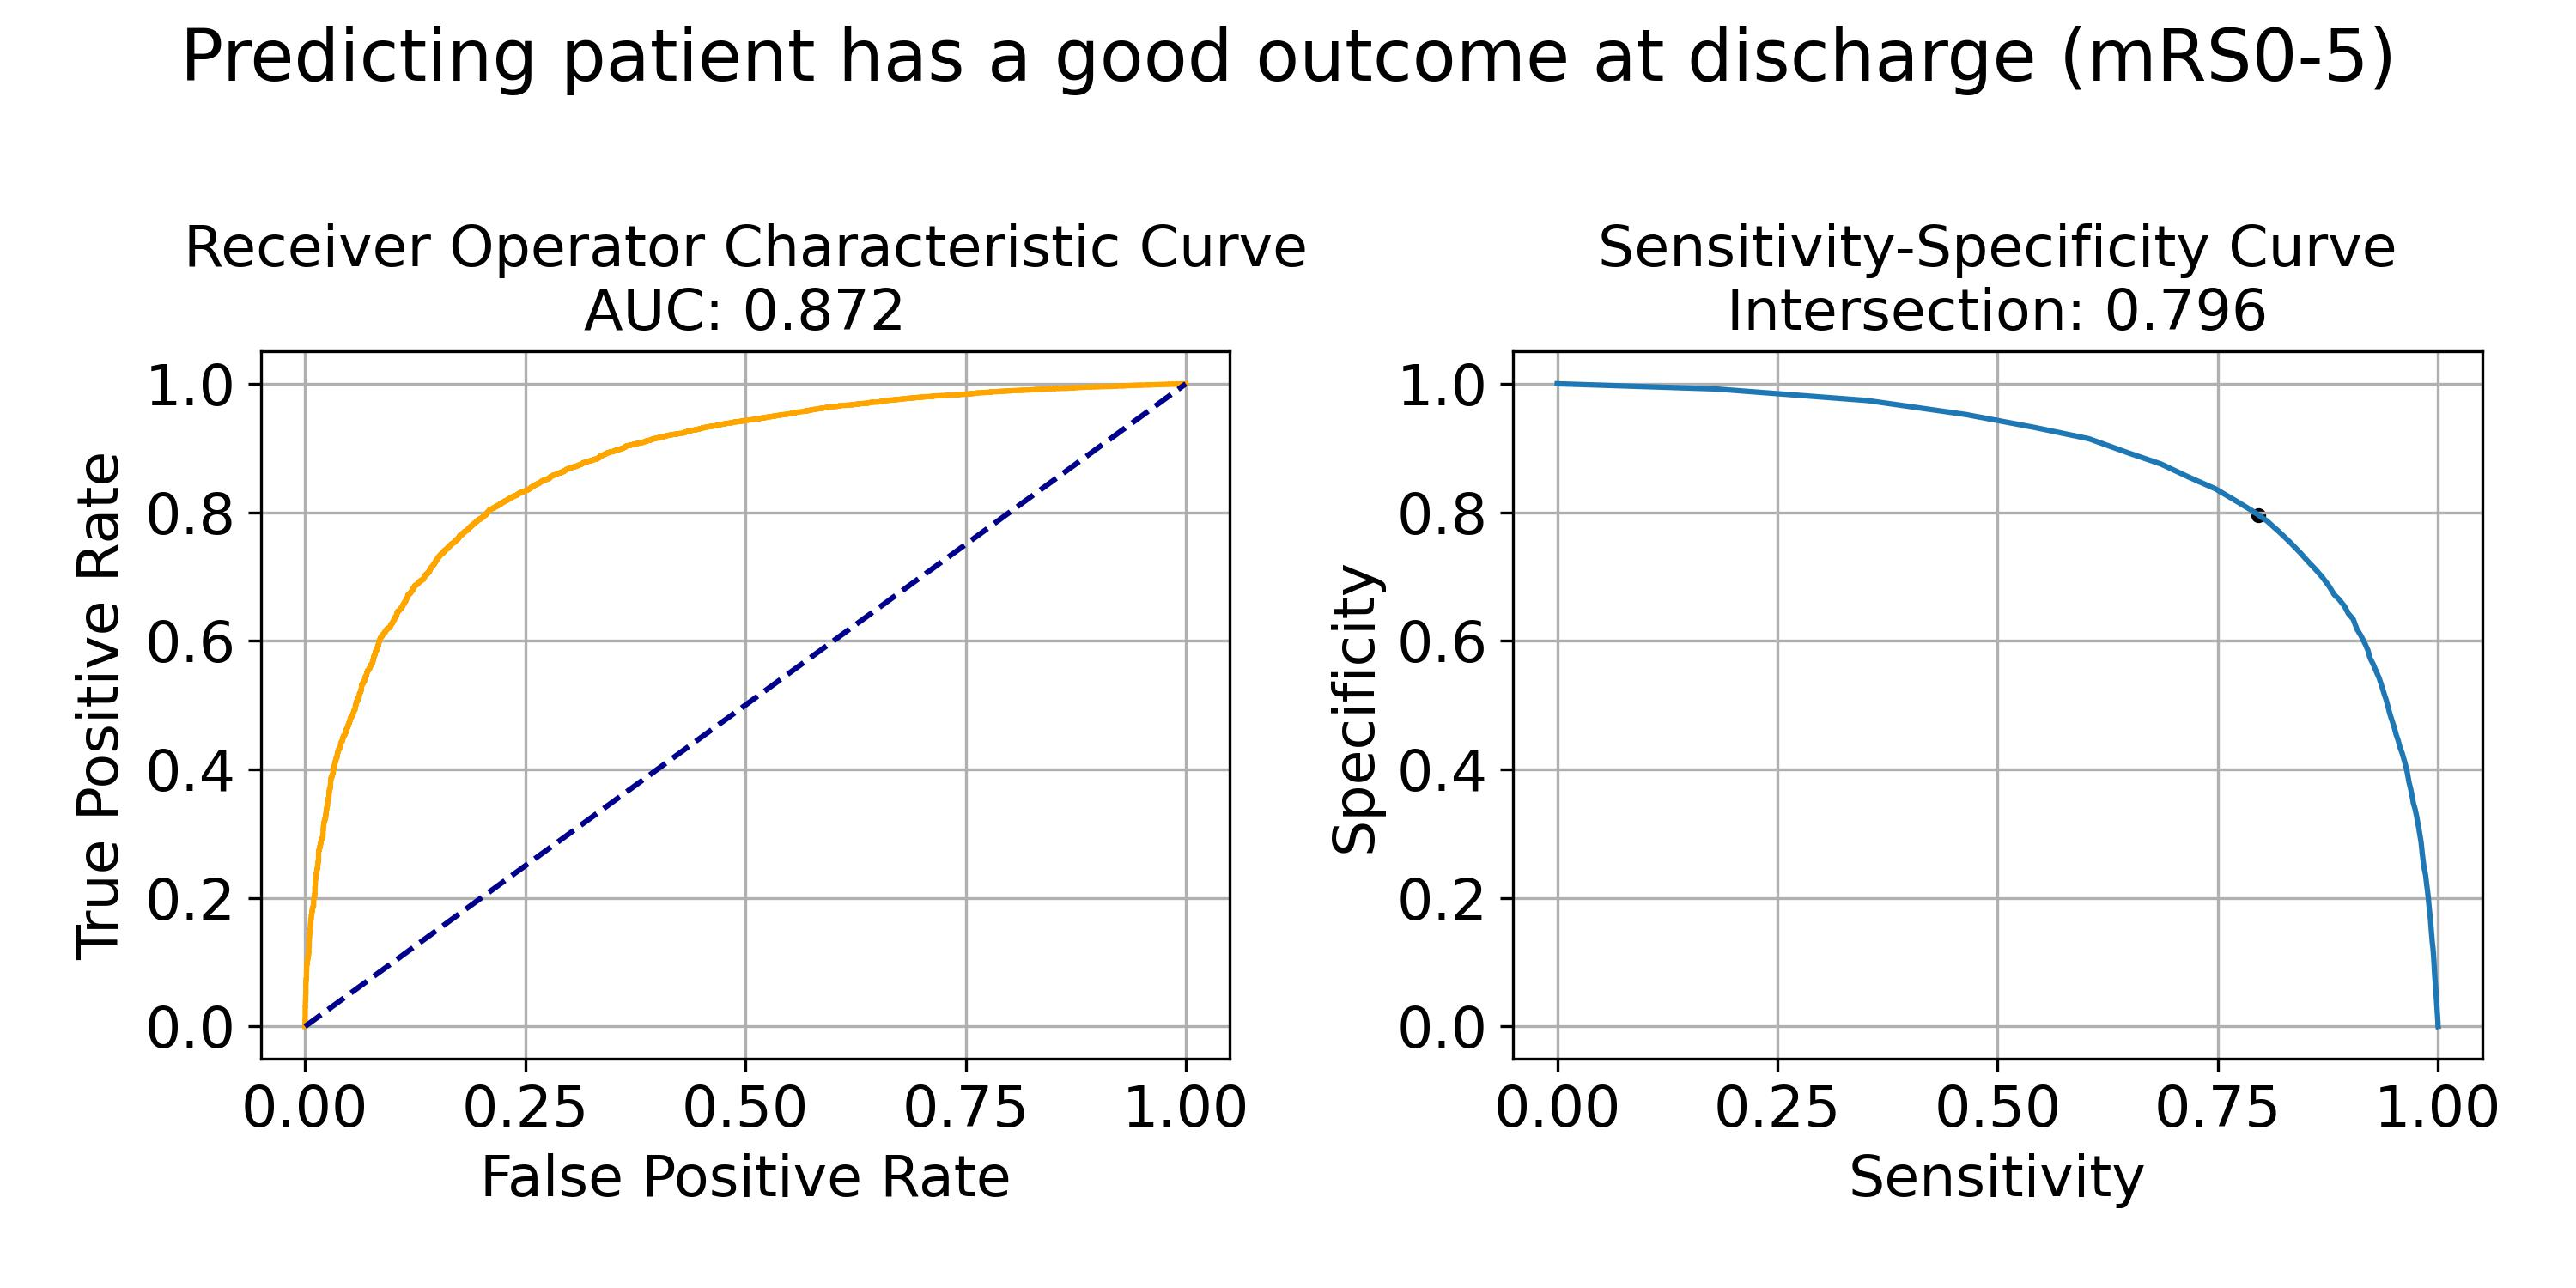
\includegraphics[width=0.5\linewidth]{./images/083_xgb_7_features_5fold_binary_roc_sens_spec_mrs5_kfold0_paper}}
    \label{fig:rocauc_ss}
  \caption{ROC AUC, and specificity and sensitivity plots for each of the mRS threshold levels to define a good outcome (for first kfold). Model has 7 inputs features.}

\end{figure}



\begin{figure}[!h]
    \centering
    \begin{subfigure}[b]{1\textwidth}
      \centering
      \includegraphics[width=1\textwidth]{./images/083_xgb_7_features_5fold_binary_shap_violin_0kfold}\\
      \caption{Kfold 1}
      \label{fig:results_waterfall}
    \end{subfigure}
\end{figure}
%    \hfill
%    \medskip
\begin{figure}[!h]\ContinuedFloat
    \begin{subfigure}[b]{1\textwidth}
      \centering    
      \includegraphics[width=1\textwidth]{./images/083_xgb_7_features_5fold_binary_shap_violin_1kfold}\\
      \caption{Kfold 2}
      \label{fig:results_waterfall}
    \end{subfigure}
\end{figure}
%    \hfill
%    \medskip
\begin{figure}[!h]\ContinuedFloat
    \begin{subfigure}[b]{1\textwidth}
      \centering
      \includegraphics[width=1\textwidth]{./images/083_xgb_7_features_5fold_binary_shap_violin_2kfold}\\
      \caption{Kfold 3}
      \label{fig:results_waterfall}
    \end{subfigure}
\end{figure}
%    \hfill
%    \medskip
\begin{figure}[!h]\ContinuedFloat
    \begin{subfigure}[b]{1\textwidth}
      \centering
      \includegraphics[width=1\textwidth]{./images/083_xgb_7_features_5fold_binary_shap_violin_3kfold}\\
      \caption{Kfold 4}
      \label{fig:results_waterfall}
    \end{subfigure}
\end{figure}
%    \hfill
%    \medskip
\begin{figure}[!h]\ContinuedFloat
    \begin{subfigure}[b]{1\textwidth}
      \centering
      \includegraphics[width=1\textwidth]{./images/083_xgb_7_features_5fold_binary_shap_violin_4kfold}\\
      \caption{Kfold 5}
      \label{fig:results_waterfall}
    \end{subfigure}
  \caption{Violin plots show SHAP values vs feature values for each feature, a sub figure for each kfold}
\end{figure}



%%%%%%%%%%%% 3.6.3  %%%%%%%%%%%%%%%%%
\subsubsection{The direct contribution of thrombolysis use to the shift in probability of a good outcome - for all definitions of a good outcome (3.6.3 extension)}

Using the counterfactual results for all of the patients in the first k-fold test set that received thrombolysis, figure \ref{fig:shap_shift_lvo_nlvo} shows a linear regression fitted to the shift in the contribution from receiving thrombolysis towards having a good outcome at discharge (mRS0-1) with respect to the onset to thrombolysis time. 

Figures \ref{fig:stats_table_common_odds_ratio} and \ref{fig:stats_table_mrs1} show that the linear regression coefficients are statistically significant. Taking mRS 0-1 as a good outcome, we found that the effect of thrombolysis had declined to zero at 328 minutes, and the effect from thrombolysis was improving odds of a good outcome by 0.90 if it were, theoretically, given at the time of stroke onset. Figure \ref{fig:shap_shift_lvo} shows results for the patient cohort with a severe stroke severity (NIHSS 11+). Figure \ref{fig:shap_shift_nlvo} shows results for the patient cohort with a mild-moderate stroke severity (NIHSS 0-10). Linear regression coefficients in both groups were statistically significant (figures \ref{fig:stats_table_common_odds_ratio} and \ref{fig:stats_table_mrs1}). We observed that the maximum theoretical effect of thrombolysis (if given at time of stroke onset) was greater for the severe stroke group (1.048 log odds for mRS0-1) than the mild-moderate stroke group (0.771 log odds for mRS0-1). However the effect of thrombolysis declined a little faster in the severe stroke group (reaching no effect at 314 minutes, compared to 351 minutes for mild-moderate stroke patients).

\begin{figure}[!ht]
    \centering
    \begin{subfigure}[b]{.7\textwidth}
      \centering
      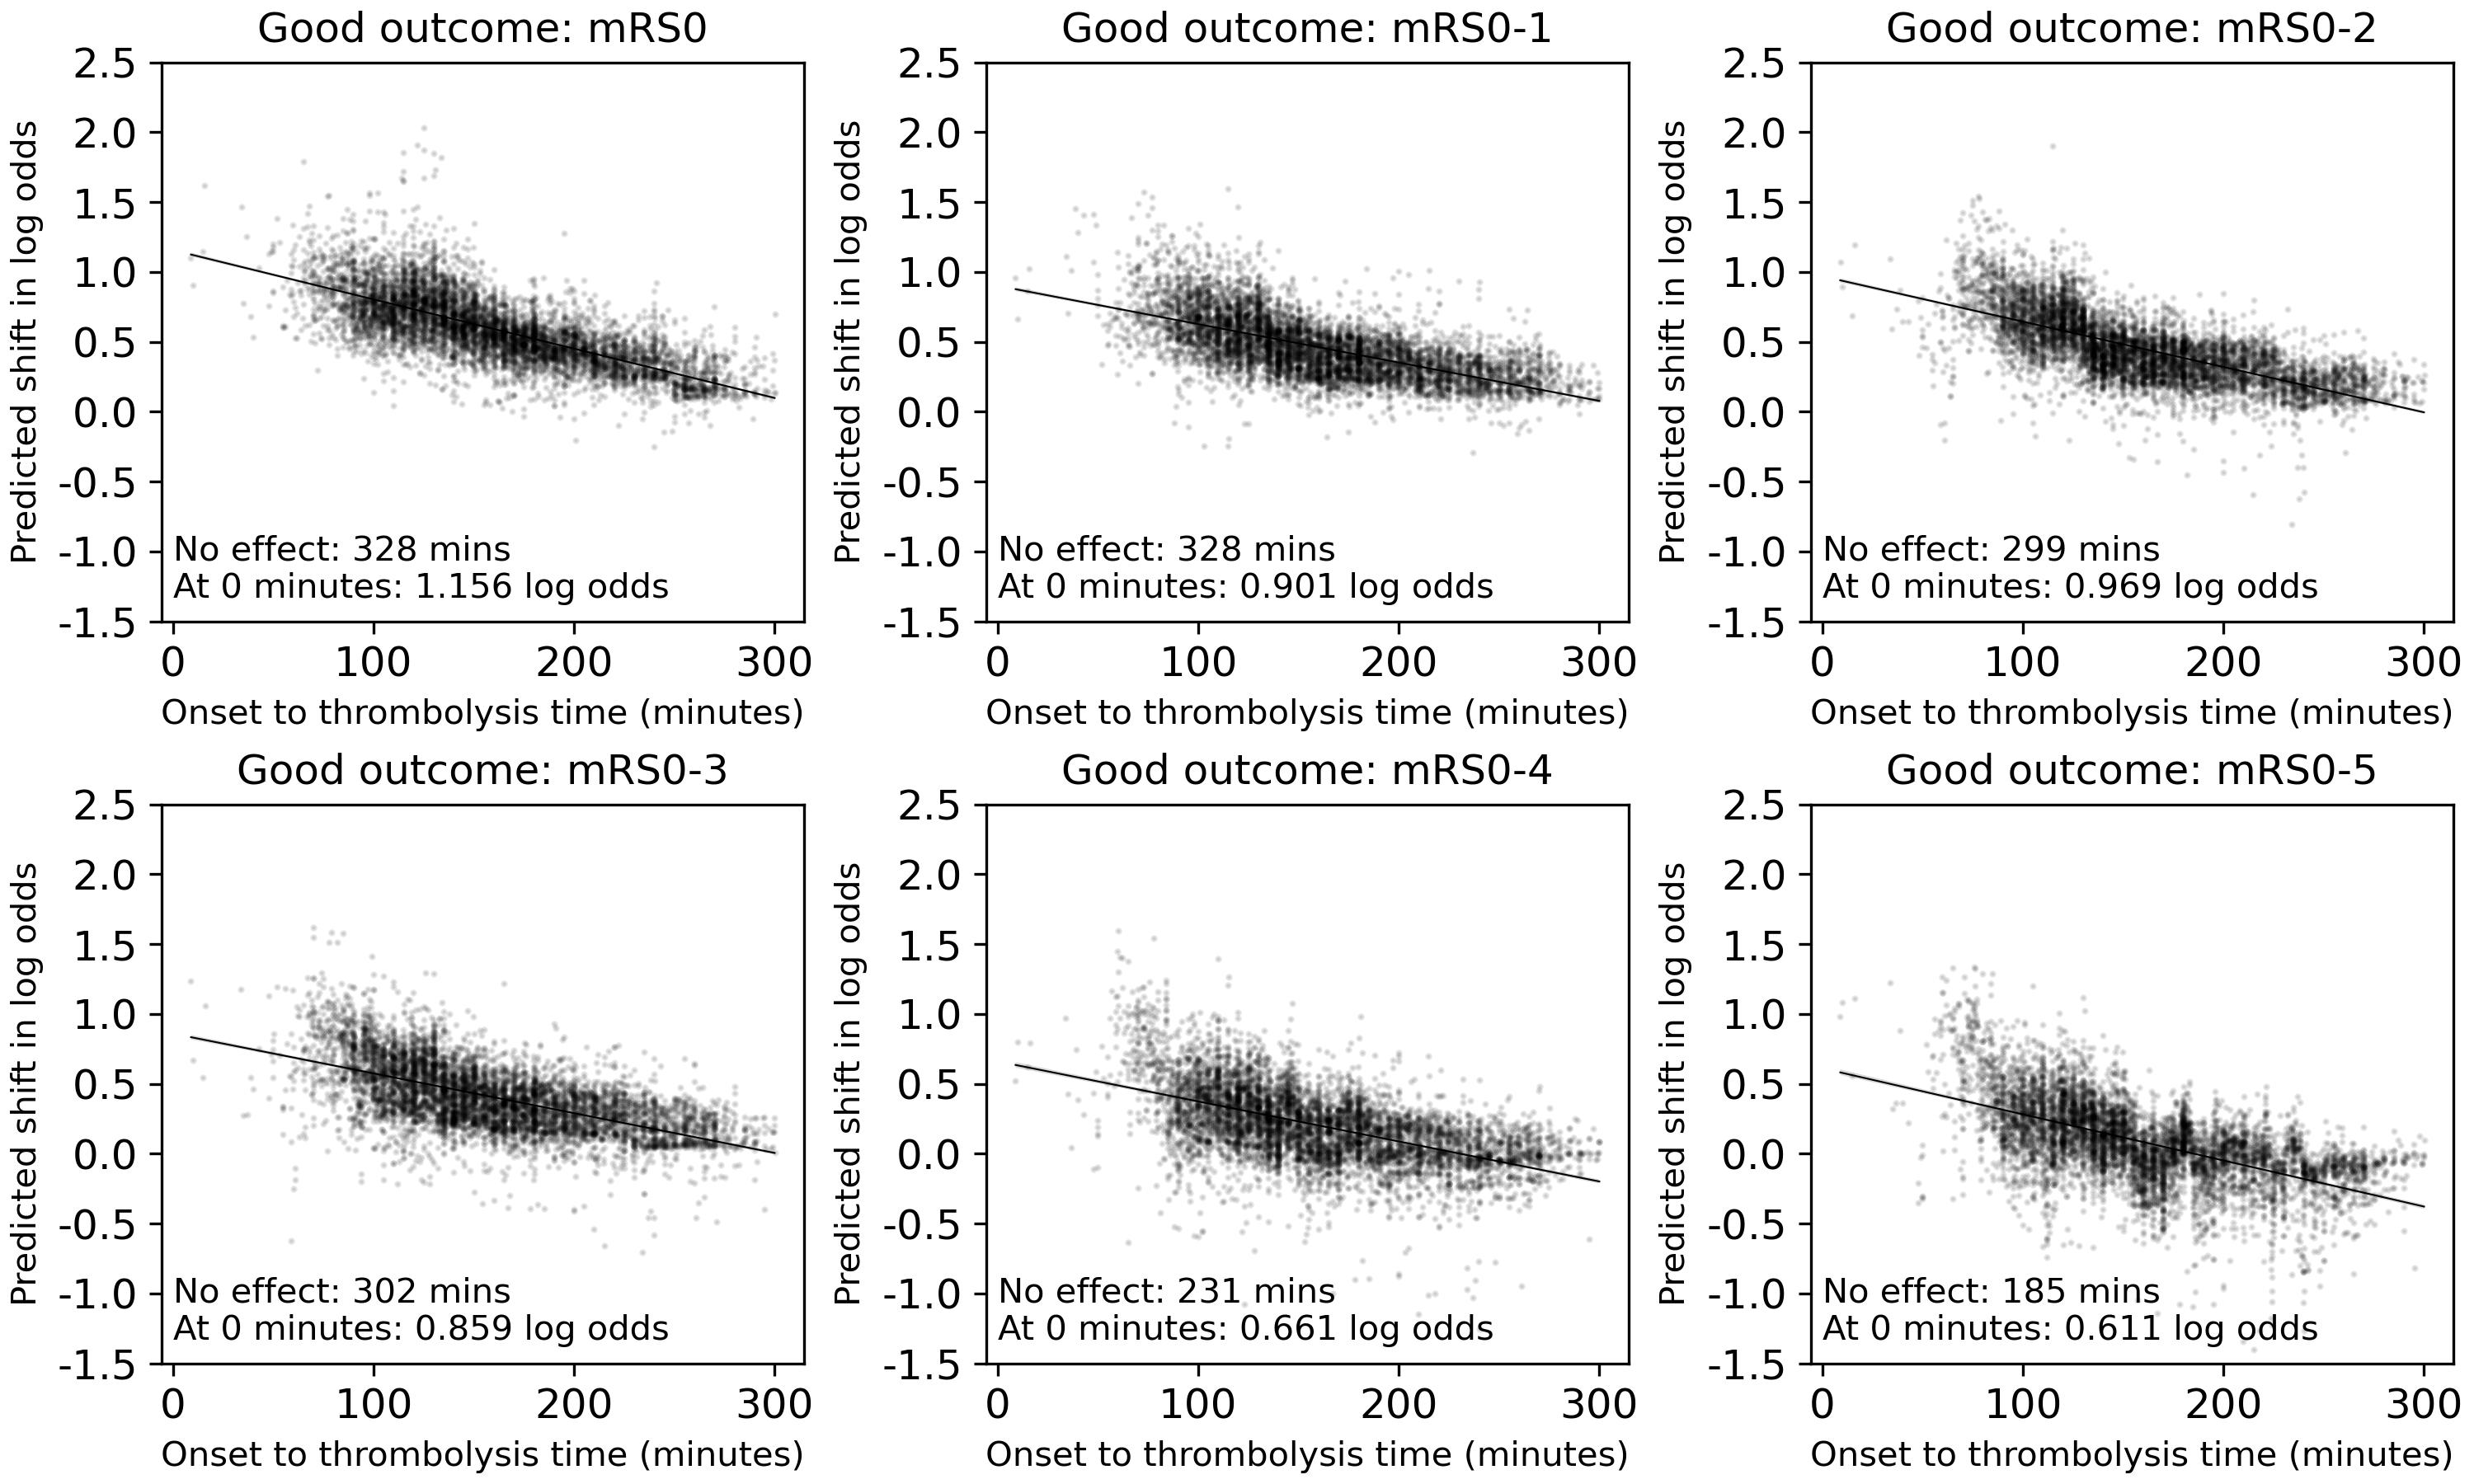
\includegraphics[width=1\textwidth]{./images/103_xgb_7_features_1fold_binary_improvement_logodds_bymRSthreshold_sns_6_subplots_nLVO_LVO_ivt_shap_paper}\\
      \caption{Patients in the test set that received thrombolysis}
      \label{fig:shap_shift_lvo_nlvo}
    \end{subfigure}
    \hfill
    \begin{subfigure}[b]{.7\textwidth}
      \centering    
      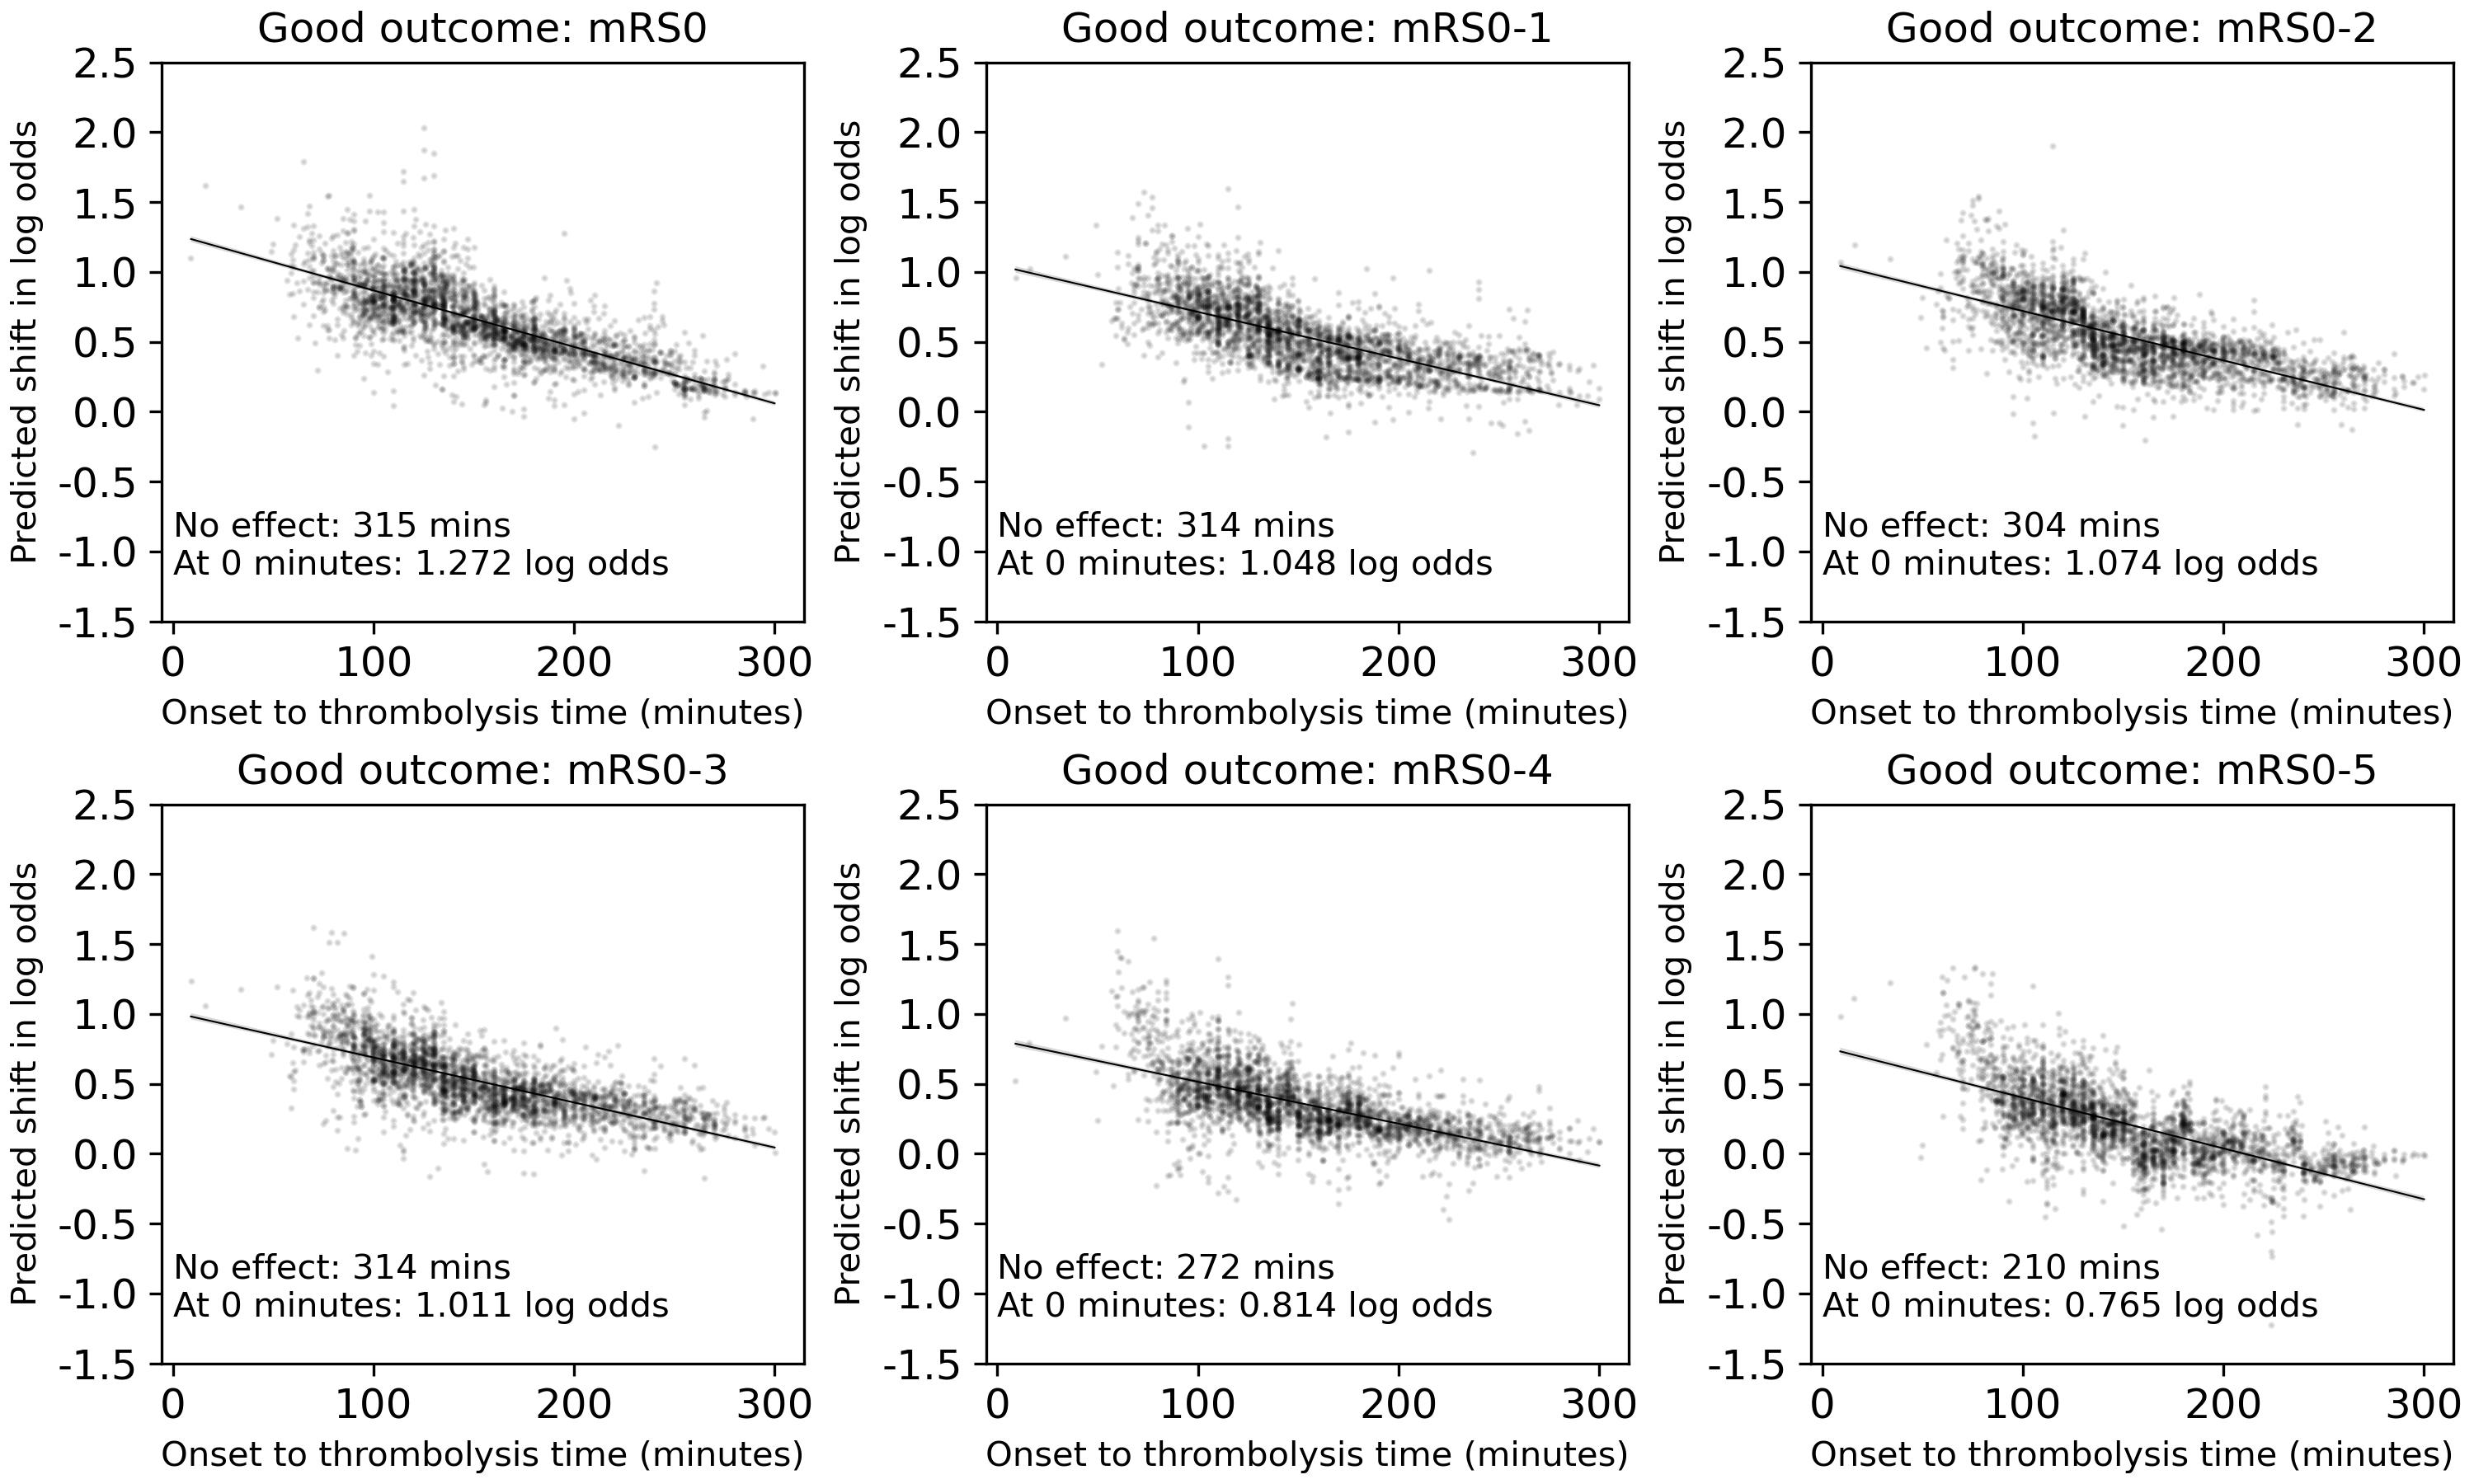
\includegraphics[width=1\textwidth]{./images/103_xgb_7_features_1fold_binary_improvement_logodds_bymRSthreshold_sns_6_subplots_LVO_ivt_shap_paper}\\
      \caption{Patients in the test set that received thrombolysis with severe stroke (NIHSS 11+)}
      \label{fig:shap_shift_lvo}
    \end{subfigure}
    \hfill
    \begin{subfigure}[b]{.7
    \textwidth}
      \centering
      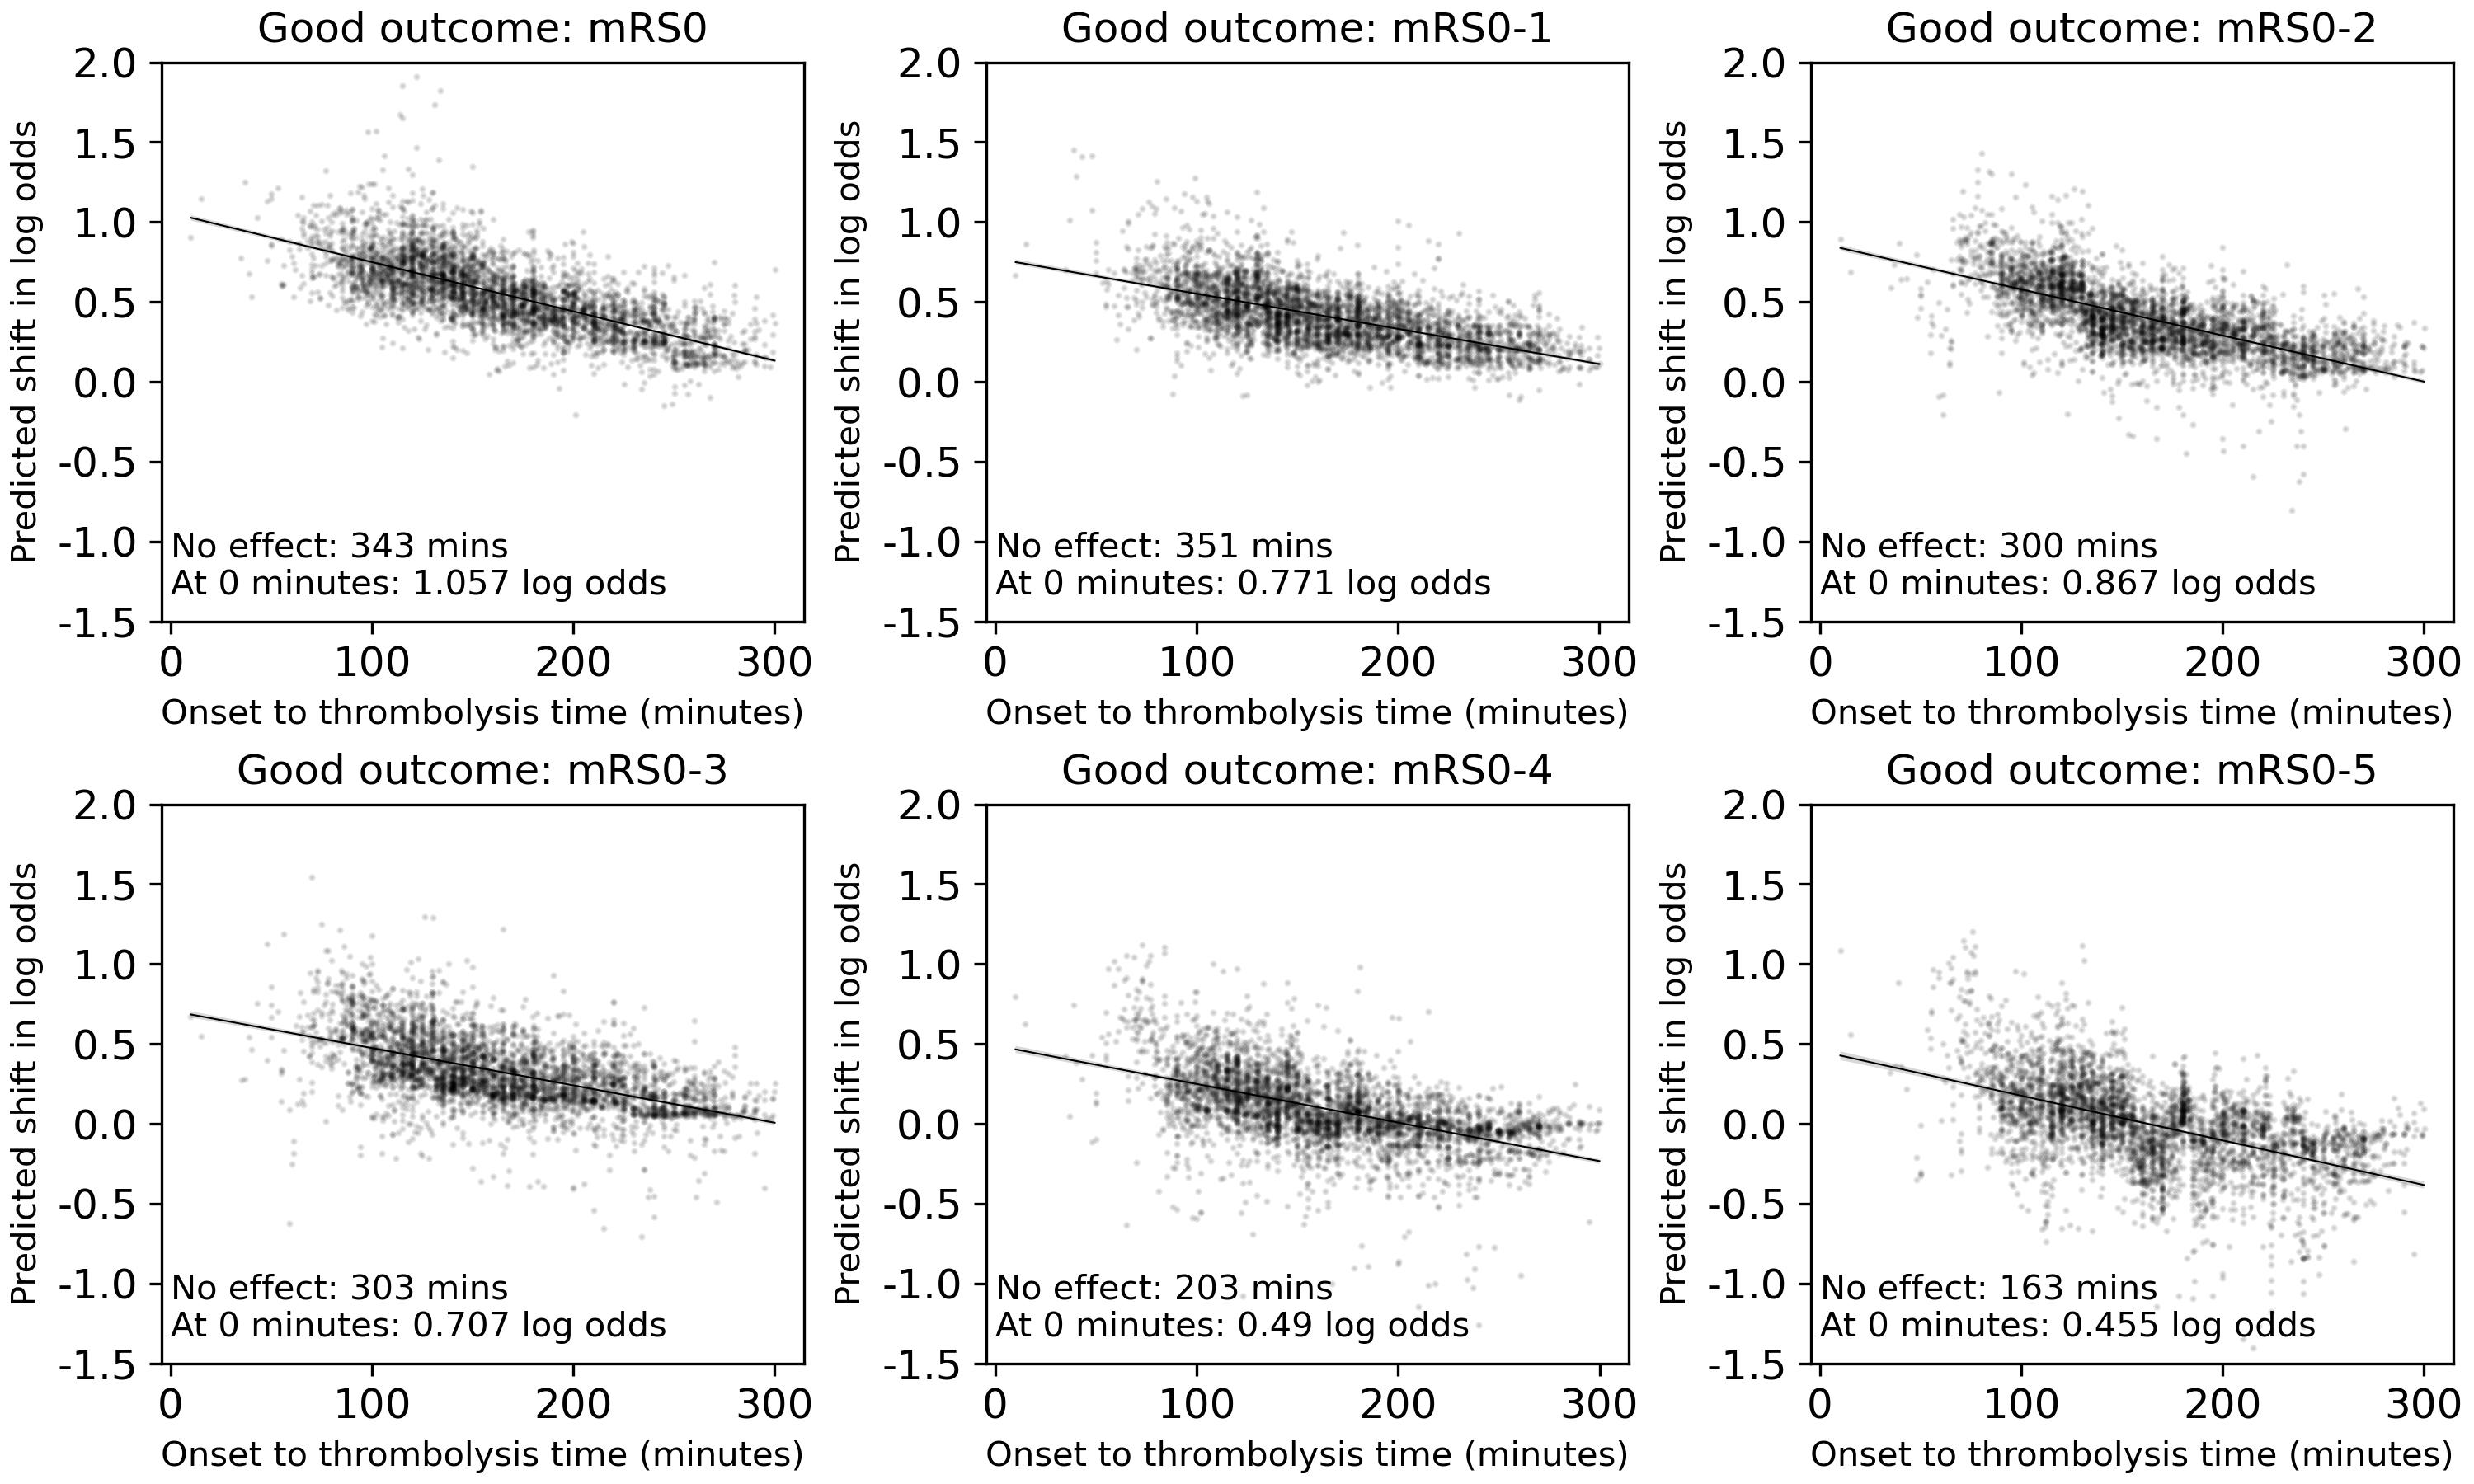
\includegraphics[width=1\textwidth]{./images/103_xgb_7_features_1fold_binary_improvement_logodds_bymRSthreshold_sns_6_subplots_nLVO_ivt_shap_paper}\\
      \caption{Patients in the test set that received thrombolysis with mild-moderate stroke (NIHSS 0-10)}
      \label{fig:shap_shift_nlvo}
    \end{subfigure}
    \label{fig:shap_shift}
    \caption{Fitting linear regression to the shift in the contribution from receiving thrombolysis towards having a good outcome at discharge with respect to the onset to thrombolysis time. A subplot for each mRS threshold used to define a good outcome.}
\end{figure}

\begin{table}[!ht]
    \caption{Fitting linear regression to the shift in the contribution from receiving thrombolysis towards having a good outcome (mRS 0-1) at discharge with respect to the onset to thrombolysis time. Linear regression statistics for different patient cohorts, and different definitions of a good outcome. We used NIHSS 0-10 to define mild-moderate strokes, and NIHSS 11+ to define severe strokes. }
%    \begin{subtable}[b]{1\textwidth}
%          \caption{Good outcome defined using all six mRS thresholds (common odds ratio).}
%    \centering
%        \begin{tabular}{lllllllll}
%        \toprule
%         & Variables & coef & std err & t & P$>$$|$t$|$ & [0.025 & 0.975] \\ 
%         \midrule
%        All ischaemic stroke & Constant  & 0.8596 & 0.004 & 202.579 & 0.000 & 0.851 & 0.868\\
%        & Onset to IVT time (mins) & -0.0031 & 2.52e-05 & -122.600 & 0.000 & -0.003 & -0.003\\ 
%        \midrule
%        Severe stroke & Constant  & 0.9971  &    0.006 &   174.202  &    0.000    &   0.986   &    1.008\\
%        & Onset to IVT time (mins) & -0.0027  &  3.3e-05 &   -83.259  &    0.000   &   -0.003    &  -0.003\\ \midrule
 %       Mild-moderate stroke & Constant & 0.7245 & 0.006 & 126.085 & 0.000 & 0.713 & 0.736\\
 %       & Onset to IVT time (mins)  &  -0.0026 &  3.33e-05 &   -78.747  &    0.000 &     -0.003  &    -0.003\\
 %       \bottomrule
 %       \end{tabular}

 %     \label{fig:stats_table_common_odds_ratio}
 %   \end{subtable}
 %   \par\bigskip % force a bit of vertical whitespace
%    \begin{subtable}[b]{1\textwidth}
%    \caption{Good outcome defined as mRS 0-1.}
    \centering
        \begin{tabular}{lllllllll}
        \toprule
         & Variables & coef & std err & t & P$>$$|$t$|$ & [0.025 & 0.975] \\ 
         \midrule
        All ischaemic stroke & Constant & 0.9012 & 0.007 & 132.519 & 0.000 & 0.888 & 0.915\\
        & Onset to IVT time (min) &  -0.0027  & 4.04e-05 & -68.058 & 0.000 & -0.003 & -0.003\\   
        \midrule
        Severe stroke & Constant & 1.0476  &    0.011  & 96.746 & 0.000 & 1.026 & 1.069\\
        & Onset to IVT time (mins) & -0.0033 &  6.67e-05  & -50.042 & 0.000 & -0.003 & -0.003\\ 
        \midrule
        Mild-moderate stroke & Constant &           0.7708 &     0.008   & 97.613 & 0.000 & 0.755 & 0.786\\
        & Onset to IVT time (mins) &  -0.0022 &   4.57e-05 & -48.109 & 0.000 & -0.002 & -0.002\\
        \bottomrule
        \end{tabular}

      \label{fig:stats_table_mrs1}
%    \end{subtable}
   
\end{table}


Here is the secondary analysis that repeats the analysis in the paper that uses the full log-odds change in achieving a given mRS threshold with and without thrombolysis (instead of the log-odds change associated with the thrombolysis use feature). Using the full model prediction, rather than isolating the effect of thrombolysis using thrombolysis SHAP, produced similar results, but with a little larger predicted effect of thrombolysis (e.g  maximum theoretical beneficial of thrombolysis of improving the log odds of being discharged mRS 0-2 of 1.1 (\textit{c.f.} 0.90 when using the isolated effect of thrombolysis from the thrombolysis SHAP values, with no-effect time being 328 minutes and 334 minutes for the isolated and full effect models).

\begin{figure}[!ht]
    \centering
    \begin{subfigure}[b]{1\textwidth}
      \centering
      \includegraphics[width=1\textwidth]{./images/103_xgb_7_features_1fold_binary_improvement_logodds_bymRSthreshold_sns_6_subplots_nLVO_LVO_total_shap_paper}\\
      \caption{Patients in the test set that received thrombolysis}
      \label{fig:shap_shift_lvo_nlvo_full_model_prediction}
    \end{subfigure}
    \hfill
    \begin{subfigure}[b]{1\textwidth}
      \centering    
      \includegraphics[width=1\textwidth]{./images/103_xgb_7_features_1fold_binary_improvement_logodds_bymRSthreshold_sns_6_subplots_LVO_total_shap_paper}\\
      \caption{Patients in the test set that received thrombolysis with severe stroke (NIHSS 11+)}
      \label{fig:shap_shift_lvo_full_model_prediction}
    \end{subfigure}
    \hfill
    \begin{subfigure}[b]{1\textwidth}
      \centering
      \includegraphics[width=1\textwidth]{./images/103_xgb_7_features_1fold_binary_improvement_logodds_bymRSthreshold_sns_6_subplots_nLVO_total_shap_paper}\\
      \caption{Patients in the test set that received thrombolysis with mild-moderate stroke (NIHSS 0-10)}
      \label{fig:shap_shift_nlvo_full_model_prediction}
    \end{subfigure}
    \label{fig:shap_shift_full_model_prediction}
    \caption{Fitting linear regression to the shift in the full model prediction from receiving thrombolysis towards having a good outcome at discharge with respect to the onset to thrombolysis time. A subplot for each mRS threshold used to define a good outcome.}
\end{figure}


\begin{table}[!ht]
%    \begin{subfigure}[b]{1\textwidth}
%    \centering
%        \begin{tabular}{lllllllll}
%        \toprule
%         & Variables & coef & std err & t & P$>$$|$t$|$ & [0.025 & 0.975] \\ 
%         \midrule
%        All ischaemic stroke & Constant  & 1.0387 & 0.008 & 138.005 & 0.000 & 1.024 & 1.053\\
%        & Onset to IVT time (mins) & -0.0036 & 4.47e-05 & -79.727 & 0.000 & -0.004 & -0.003\\ 
%        \midrule
%        Severe stroke & Constant  & 1.2973  &    0.011 &   119.862  &    0.000    &   1.276 & 1.319\\
%        & Onset to IVT time (mins) & -0.0042  &  6.67e-05 &   -63.065  &    0.000   &   -0.004    &  -0.004\\ \midrule
%        Mild-moderate stroke & Constant & 0.7803 & 0.010 & 80.932 & 0.000 & 0.761 & 0.799\\
%        & Onset to IVT time (mins)  &  -0.0027 &  5.58e-05 &   -48.286  &    0.000 &     -0.003  &    -0.003\\
%        \bottomrule
%        \end{tabular}
%      \caption{Good outcome defined using all six mRS thresholds (common odds ratio).}
%      \label{fig:stats_table_common_odds_ratio_full_model_prediction}
%    \end{subfigure}
%    \par\bigskip % force a bit of vertical whitespace
%    \begin{subfigure}[b]{1\textwidth}
    \centering
        \begin{tabular}{lllllllll}
        \toprule
         & Variables & coef & std err & t & P$>$$|$t$|$ & [0.025 & 0.975] \\ 
         \midrule
        All ischaemic stroke & Constant & 1.0992 & 0.016 & 68.965 & 0.000 & 1.068 & 1.130\\
        & Onset to IVT time (min) &  -0.0033  & 9.46e-05 & -34.778 & 0.000 & -0.003 & -0.003\\   
        \midrule
        Severe stroke & Constant & 1.3797  & 0.027  & 51.601 & 0.000 & 1.327 & 1.432\\
        & Onset to IVT time (mins) & -0.0044 &  0.000  & -26.845 & 0.000 & -0.005 & -0.004\\ 
        \midrule
        Mild-moderate stroke & Constant &           0.8494 & 0.018   & 46.756 & 0.000 & 0.814 & 0.885\\
        & Onset to IVT time (mins) &  -0.0022 &   0.000 & -21.301 & 0.000 & -0.002 & -0.002\\
        \bottomrule
        \end{tabular}
      \label{fig:stats_table_mrs1_full_model_prediction}
%    \end{subfigure}
    \caption{Fitting linear regression to the shift in the full model prediction from receiving thrombolysis towards having a good outcome (mRS 0-1) at discharge with respect to the onset to thrombolysis time. Linear regression statistics for different patient cohorts, and different definitions of a good outcome. We used NIHSS 11+ to define a severe stroke, and NIHSS 0-10 to define mild-moderate stroke.}
\end{table}




%\FloatBarrier

%TC:endignore

% Word counts - Don't count these!
%TC:ignore
%\section{Word counts}
%\detailtexcount{main}
%TC:endignore


\end{document}